%%%%%%%%%%%%%%%%%%%%%%%%%%%%%%%%%%%%%%%%%%%%%%%%%%%%%%%%%%%%%%%%%%%%%%%%
% Plantilla TFG/TFM
% Escuela Politécnica Superior de la Universidad de Alicante
% Realizado por: Jose Manuel Requena Plens
% Contacto: info@jmrplens.com / Telegram:@jmrplens
%%%%%%%%%%%%%%%%%%%%%%%%%%%%%%%%%%%%%%%%%%%%%%%%%%%%%%%%%%%%%%%%%%%%%%%%

\chapter{Resultados}
\label{resultados}
\section{Método por parcelas}
\subsection{Optimización}
\par La optimización de los datos de entrada tiene su base en la elección de las variables de entrada y de los sets de parcelas de entrenamiento y test. Los mejores resultados para todos los casos el uso de un conjunto de 6 parcelas para entrenamiento y 1 para la evaluación, y como datos de entrada al sistema todos los mencionados anteriormente: media por día y parcela de VV, VH y ratio VH/VV y la desviación estándar de cada uno de ellos. En cuanto a la optimización del regresor, se basa en la determinación del número de árboles que lo componen. La relación entre el número de árboles para un modelo y el coeficiente de determinación es un buen descriptor para la elección de este parámetro, como se presenta en la imagen de ejemplo \ref{fig:opt_parcl} con el caso de salida \gls{bbch}. En ella, se puede ver que una vez alcanzado cierto nivel de coeficiente, la mejora de este en relación al aumento del número de árboles no es significativa con respecto al costo computacional y a la complejidad del sistema que se crea. 
\begin{figure}[h]
    \centering
    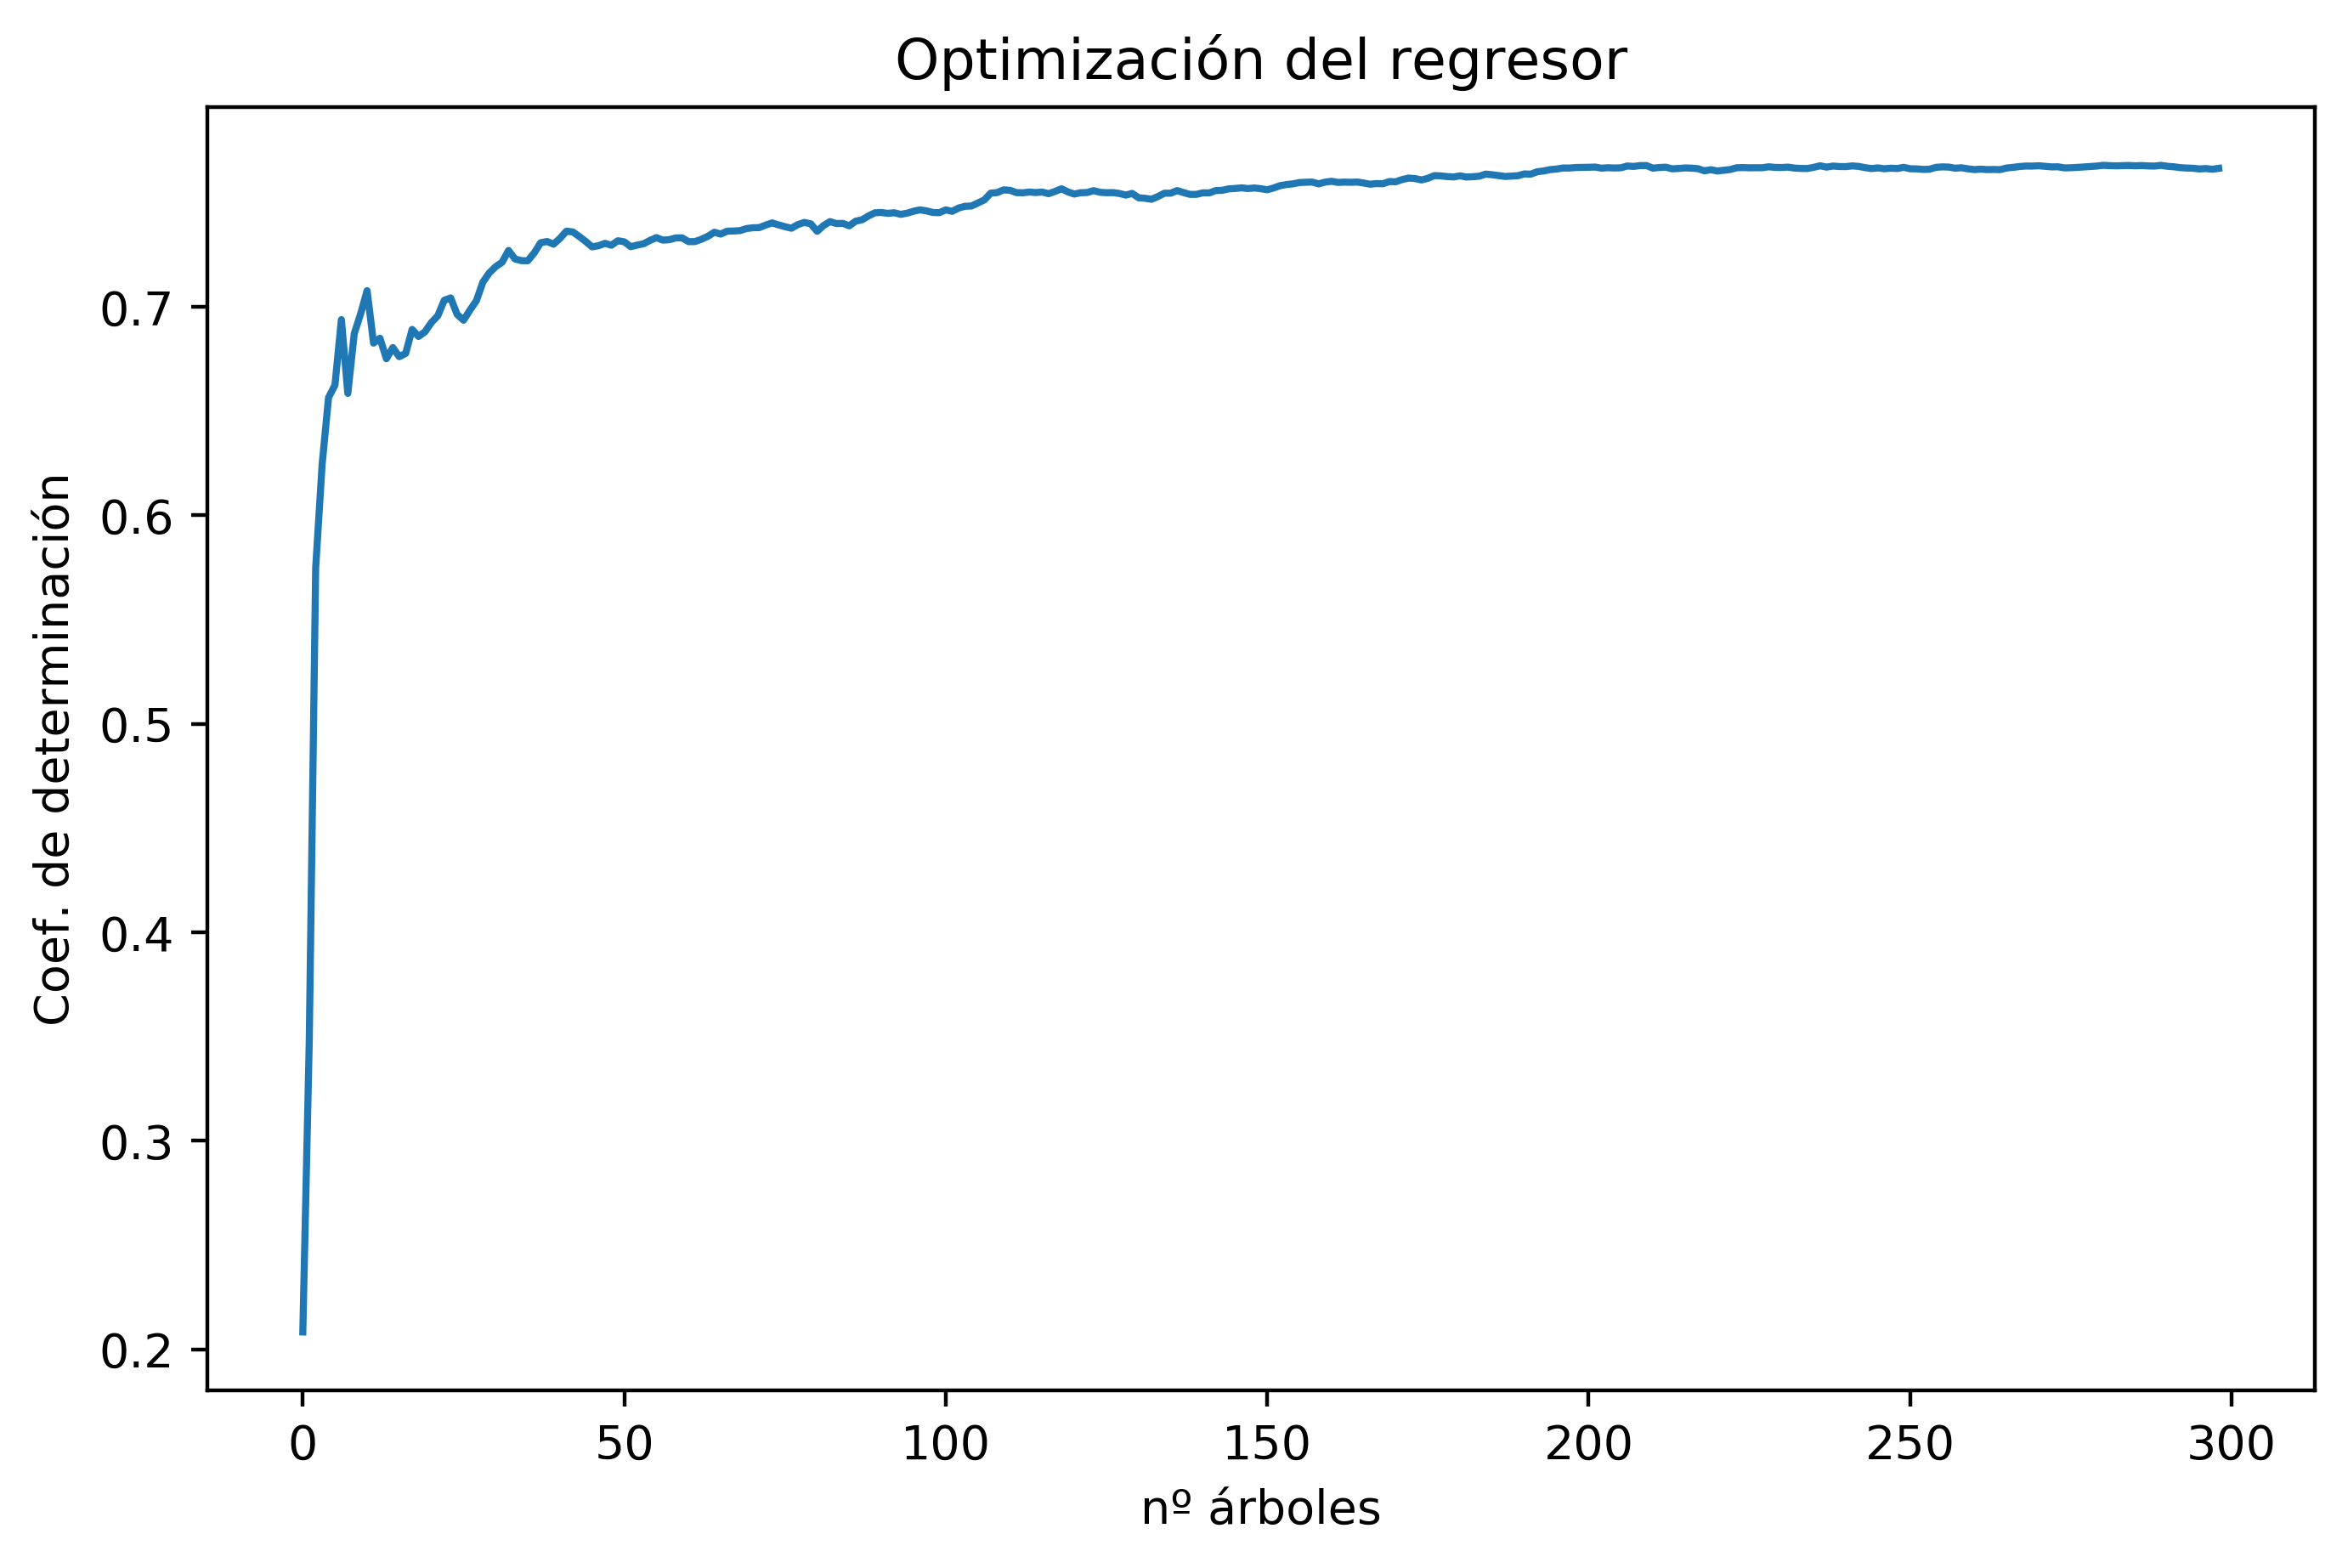
\includegraphics[height=9cm]{archivos/tfg/Mean/opt_tree_bbch_mean} 
    \caption{Optimización del número de árboles para \gls{rfr} en el modelo de salida \gls{bbch}\label{fig:opt_parcl}}
    
\end{figure}

\par Finalmente, los parámetros utilizados en este método para cada caso se presentan en la tabla \ref{tab:opt_parcl}, donde se pueden ver: la parcela utilizada para el periodo de test del modelo; siendo el resto de parcelas utilizadas en el entrenamiento, y el número de árboles óptimo para \gls{rfr}, de acuerdo con la evolución del coeficiente de determinación para cada caso.

\begin{table}[h]
\centering
\begin{tabular}{l|ccc}
                  & \gls{bbch}     & Altura   & \gls{bbch}\&Altura \\ \hline
Parcela de test   & `Mínima' & `Puntal' & `Mínima'     \\
Número de árboles & 42       & 77       & 54          
\end{tabular}
\caption{Parámetros de optimización de entrada y modelo
\label{tab:opt_parcl}}
\end{table}

\par Como se puede observar, los 3 casos de este método constan de un número óptimo de árboles de, al menos, el mismo orden. Cabe destacar que el aumento de complejidad en el modelo, sobre todo en el caso de la altura como salida del sistema.  
\subsection{Salidas del modelo}
\subsubsection{Salidas de función de densidad de probabilidad}
Como ya se ha comentado, las salidas del modelo son por defecto predicciones únicas, pero el marco de trabajo anterior demanda salidas en formato \gls{pdf} para ser integradas con el resto del modelo. En las figuras \ref{fig:pdf_b} (modelo de salida \gls{bbch}), \ref{fig:pdf_h} (modelo de salida altura) y \ref{fig:pdf_bh} (modelo de ambas salidas) se puede apreciar cómo son algunas de estas salidas, siendo ejemplos extraídos a partir de los mismos datos para los 3 casos estudiados. 
\\
\par Las \gls{pdf}s se presentan normalizadas con respecto a la salida con mayor probabilidad. En estos ejemplos se puede ver como, aunque hay una salida que predomina con respecto al resto, no se excluyen las demás soluciones posibles. Esto facilita la integración con el modelo de predicción temporal ya que se pueden combinar ambas salidas \gls{pdf} para ver dónde coinciden y con qué probabilidad. En general, los resultados de la predicción temporal son bastante certeros, con oportunidad de fallo para ajustes finos en cultivos que hayan podido sufrir retrasos o adelantos en su desarrollo típico. Es ahí donde la contribución de este modelo es importante, aportando información extra en tiempo real y creando una predicción de cuáles serían los posibles estados de desarrollo en los que se encuentra el cultivo según la información actual de satélite. 
\\
% Una figura con dos imágenes
\begin{figure}[H]
\centering
\begin{subfigure}{0.6\textwidth}
  \centering
  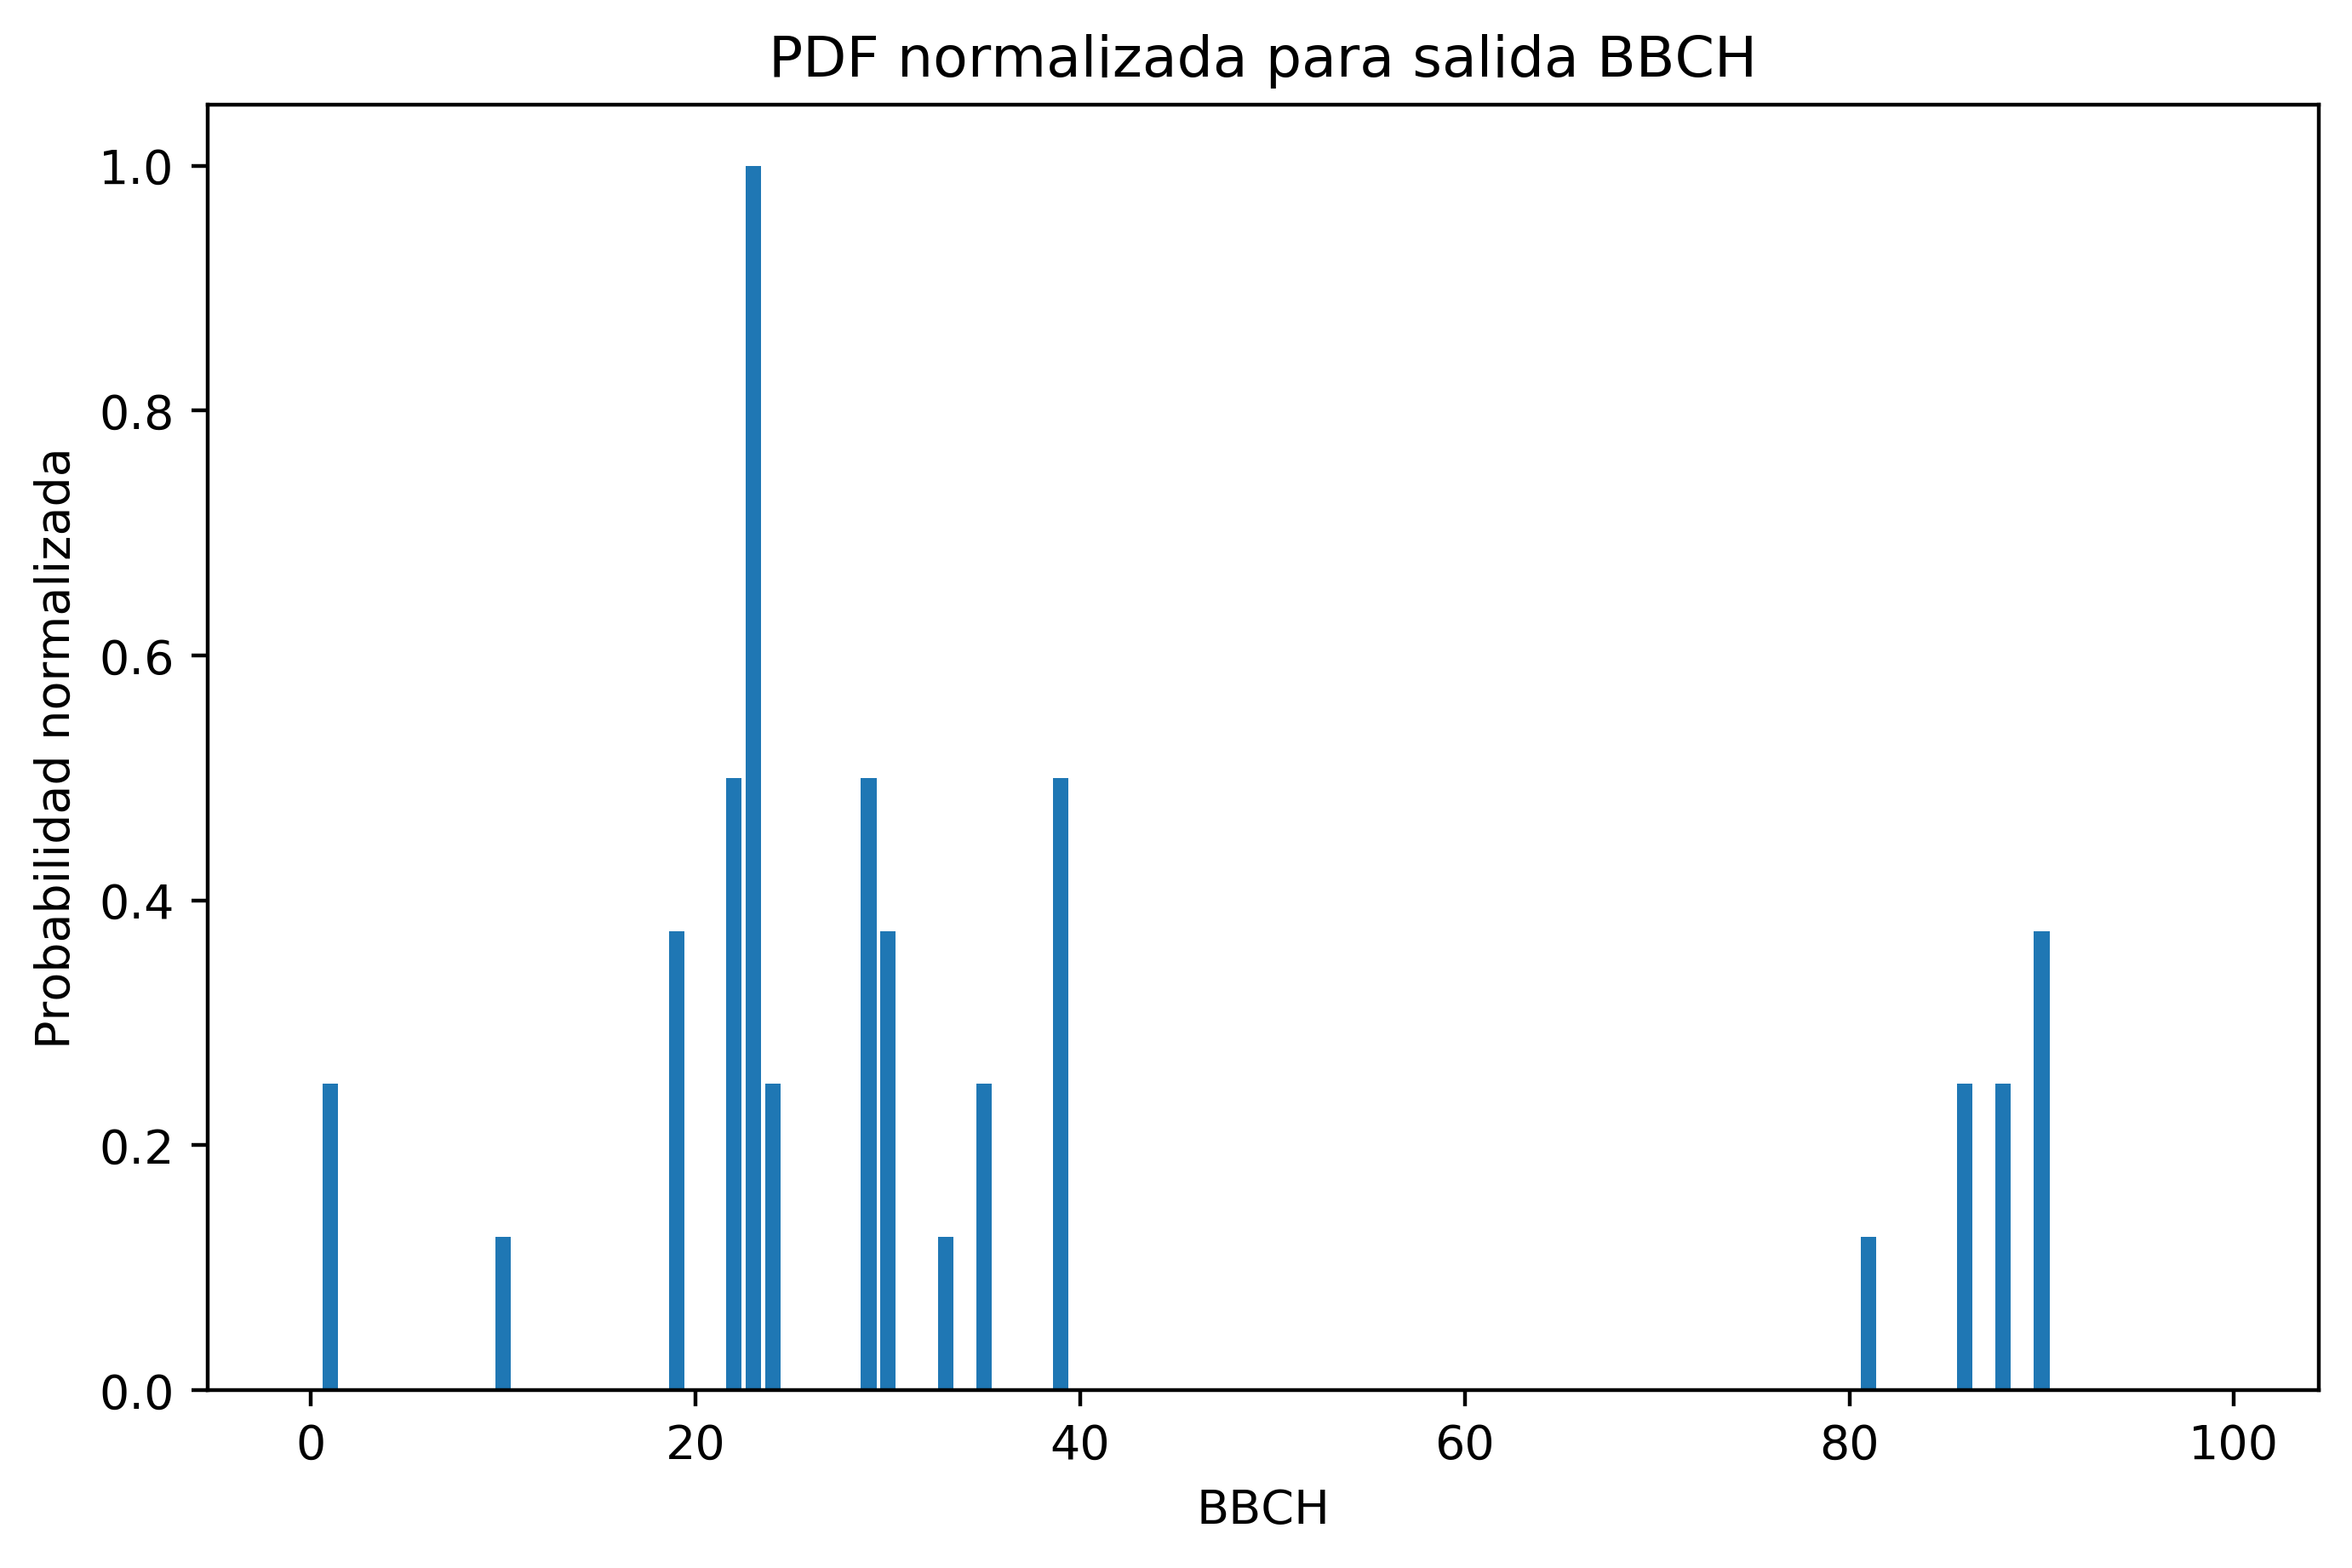
\includegraphics[width=0.95\linewidth]{archivos/tfg/Mean/TEST_PARC_PDF}
  \caption{Ejemplo del modelo de doble salida: \gls{pdf} estimación de \gls{bbch}\label{fig:pdf_b}}
\end{subfigure}
\begin{subfigure}{0.6\textwidth}
  \centering
  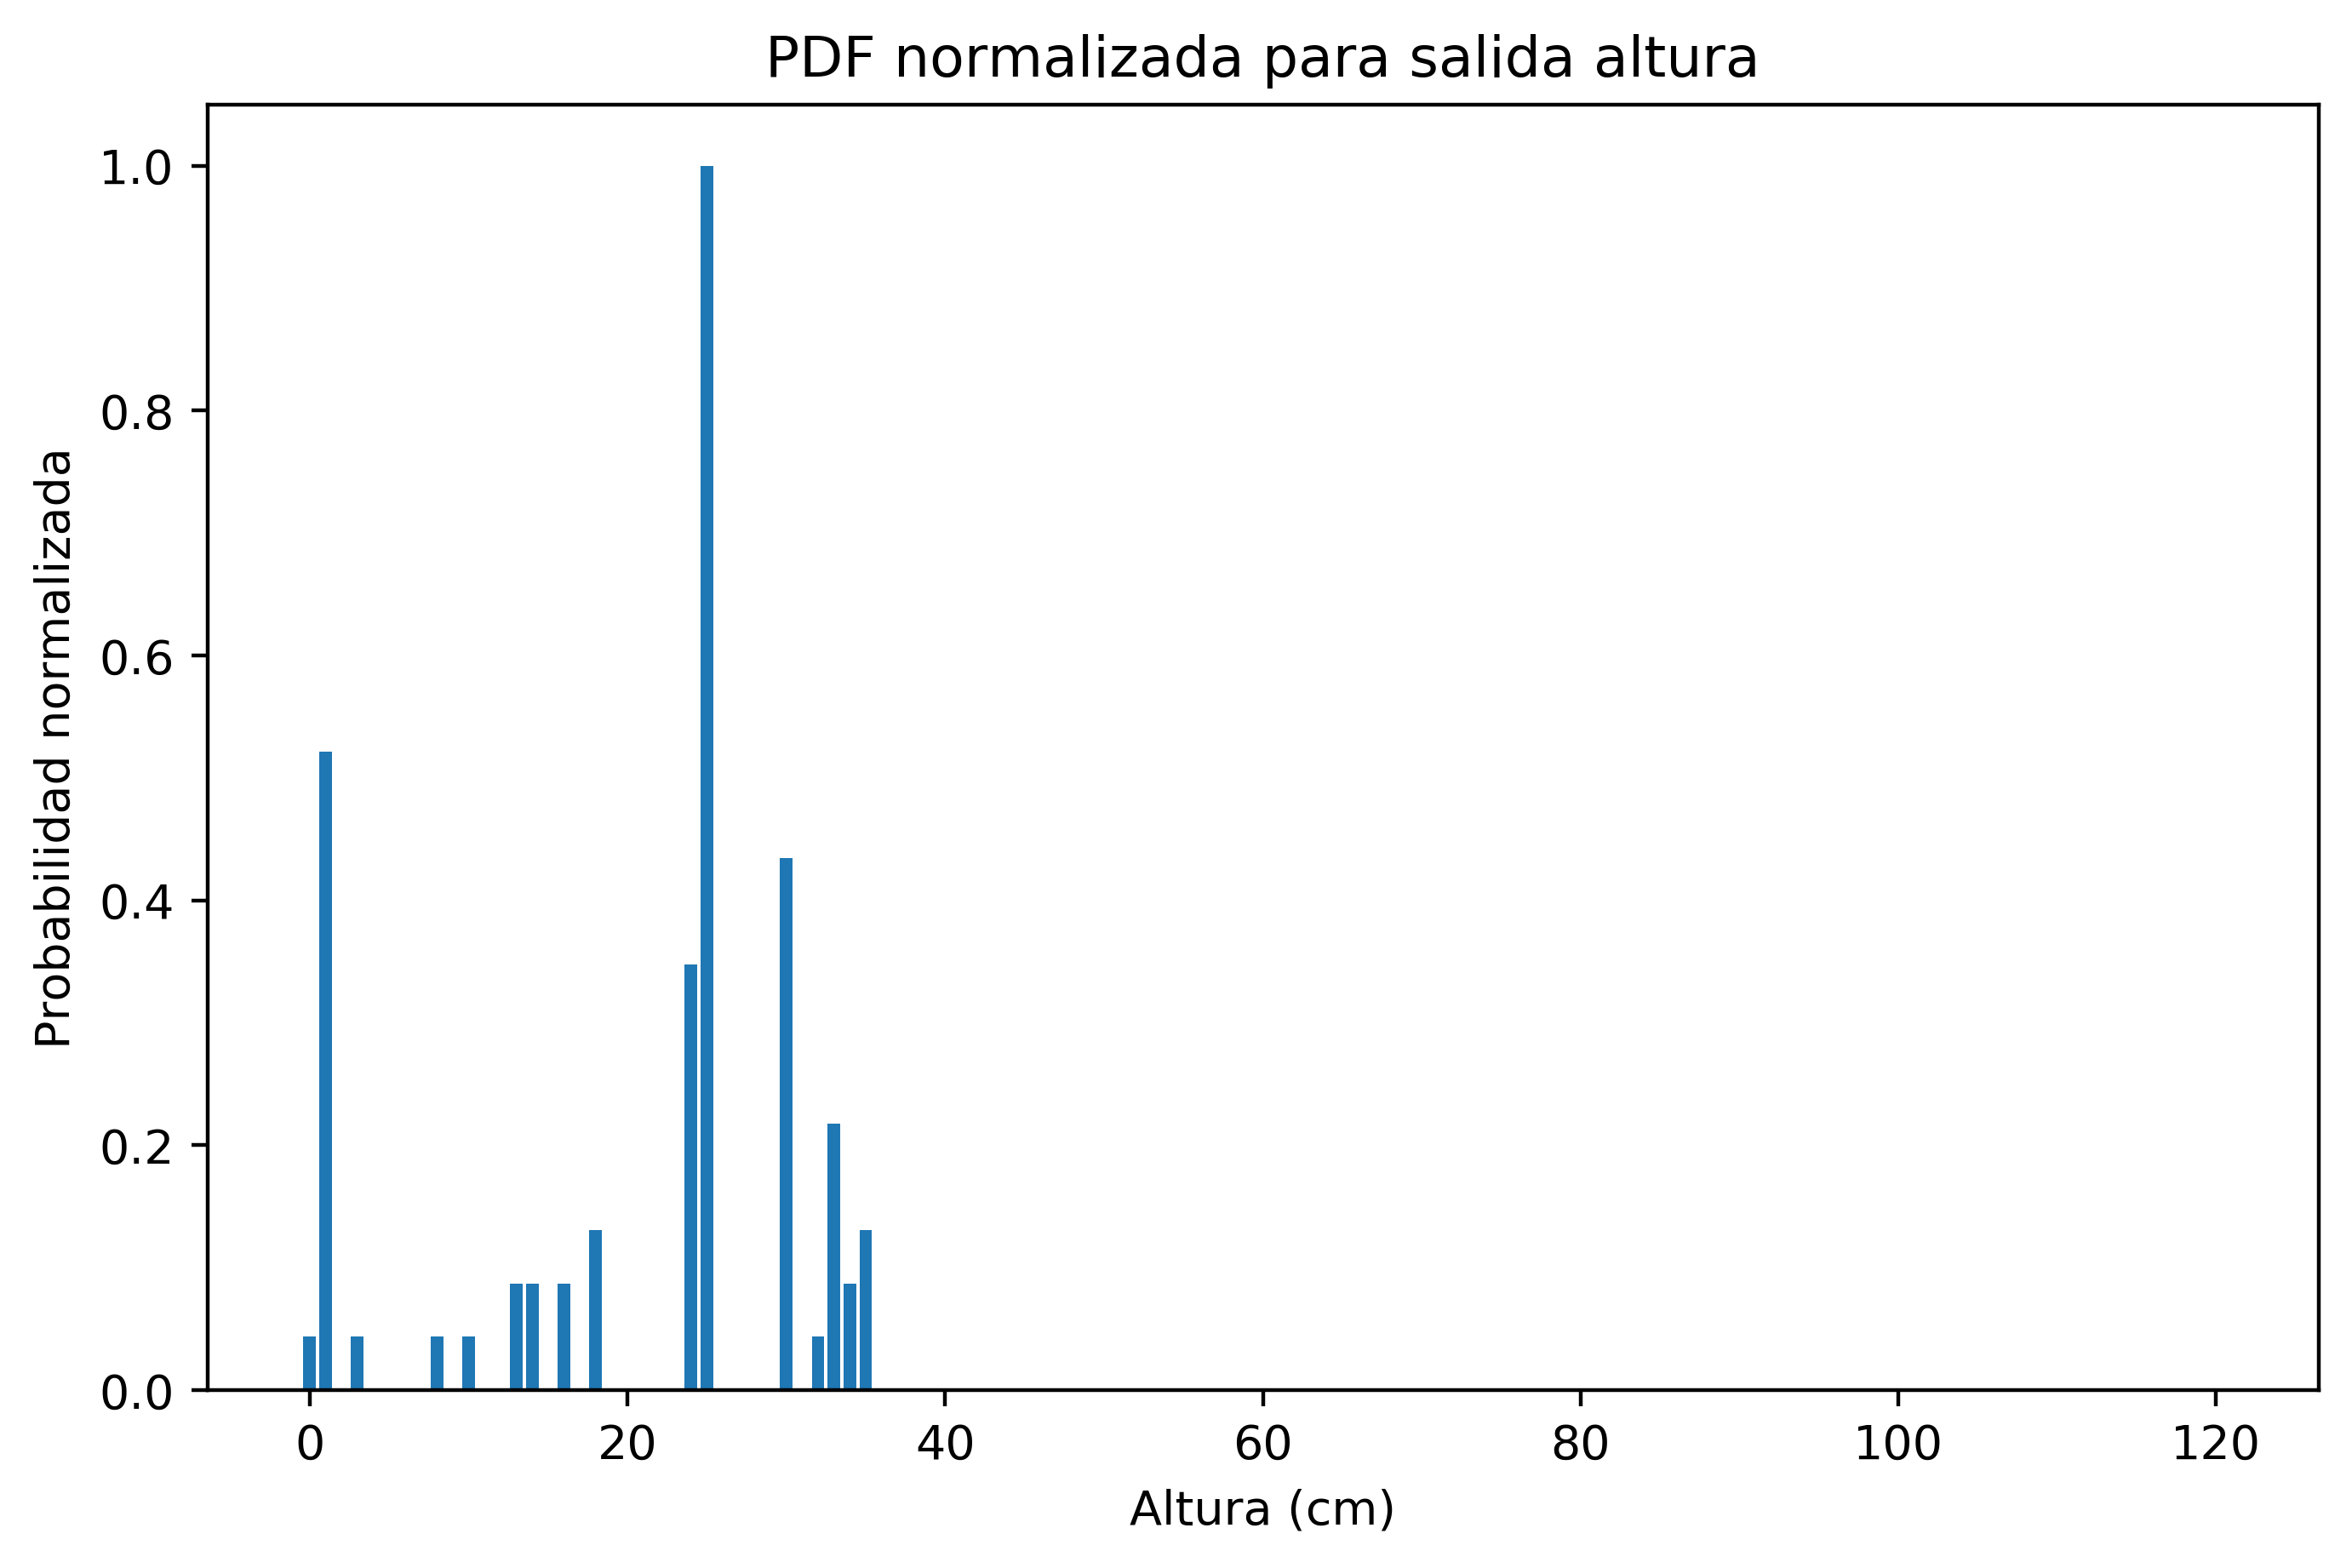
\includegraphics[width=0.95\linewidth]{archivos/tfg/Mean/TEST_PARC_PDF_H}
  \caption{Ejemplo del modelo de doble salida: \gls{pdf} estimación de altura\label{fig:pdf_h}}
\end{subfigure}
\caption{Ejemplo de salidas \gls{pdf} normalizadas del modelo para estimación de \gls{bbch} y la altura. \label{fig:pdf_bh}}
\end{figure}
\par Las 3 figuras \ref{fig:pdf_b}, \ref{fig:pdf_h} y \ref{fig:pdf_bh} han sido generadas con los mismos datos de entrada, es decir, los mismos datos de satélite en la misma parcela y fecha, por lo que las salidas para los modelos generados de estimación de \gls{bbch} (Figura \ref{fig:pdf_b}) y altura (Figura \ref{fig:pdf_h}) como modelos independientes se pueden comparar con las salidas del modelo de estimación de ambas (Figura \ref{fig:pdf_bh}). La principal diferencia que encontramos entre los mismos tipos de datos de salida para cada modelo es que, en general, las salidas individuales presentan una estimación principal con una diferencia de probabilidad mucho mayor con respecto al resto que las estimaciones del modelo de doble salida. El rango para cada salida se mantiene bastante similar en ambos modelos, además del valor con la probabilidad más alta, aunque la disminución de diferencias con las demás estimaciones, sobre todo en el caso de la altura (\ref{fig:sub2}), indica que ese sistema es menos preciso y estable. El hecho de que sea la salida de la altura la que se vea más perjudicada en este modelo de dos salidas puede deberse a que la optimización de este, en cuanto a número de árboles del regresor, es más similar, y por lo tanto más beneficiosa, con respecto al caso individual de estimación de \gls{bbch}.

% Una figura con dos imágenes
\begin{figure}[H]
\centering
\begin{subfigure}{0.6\textwidth}
  \centering
  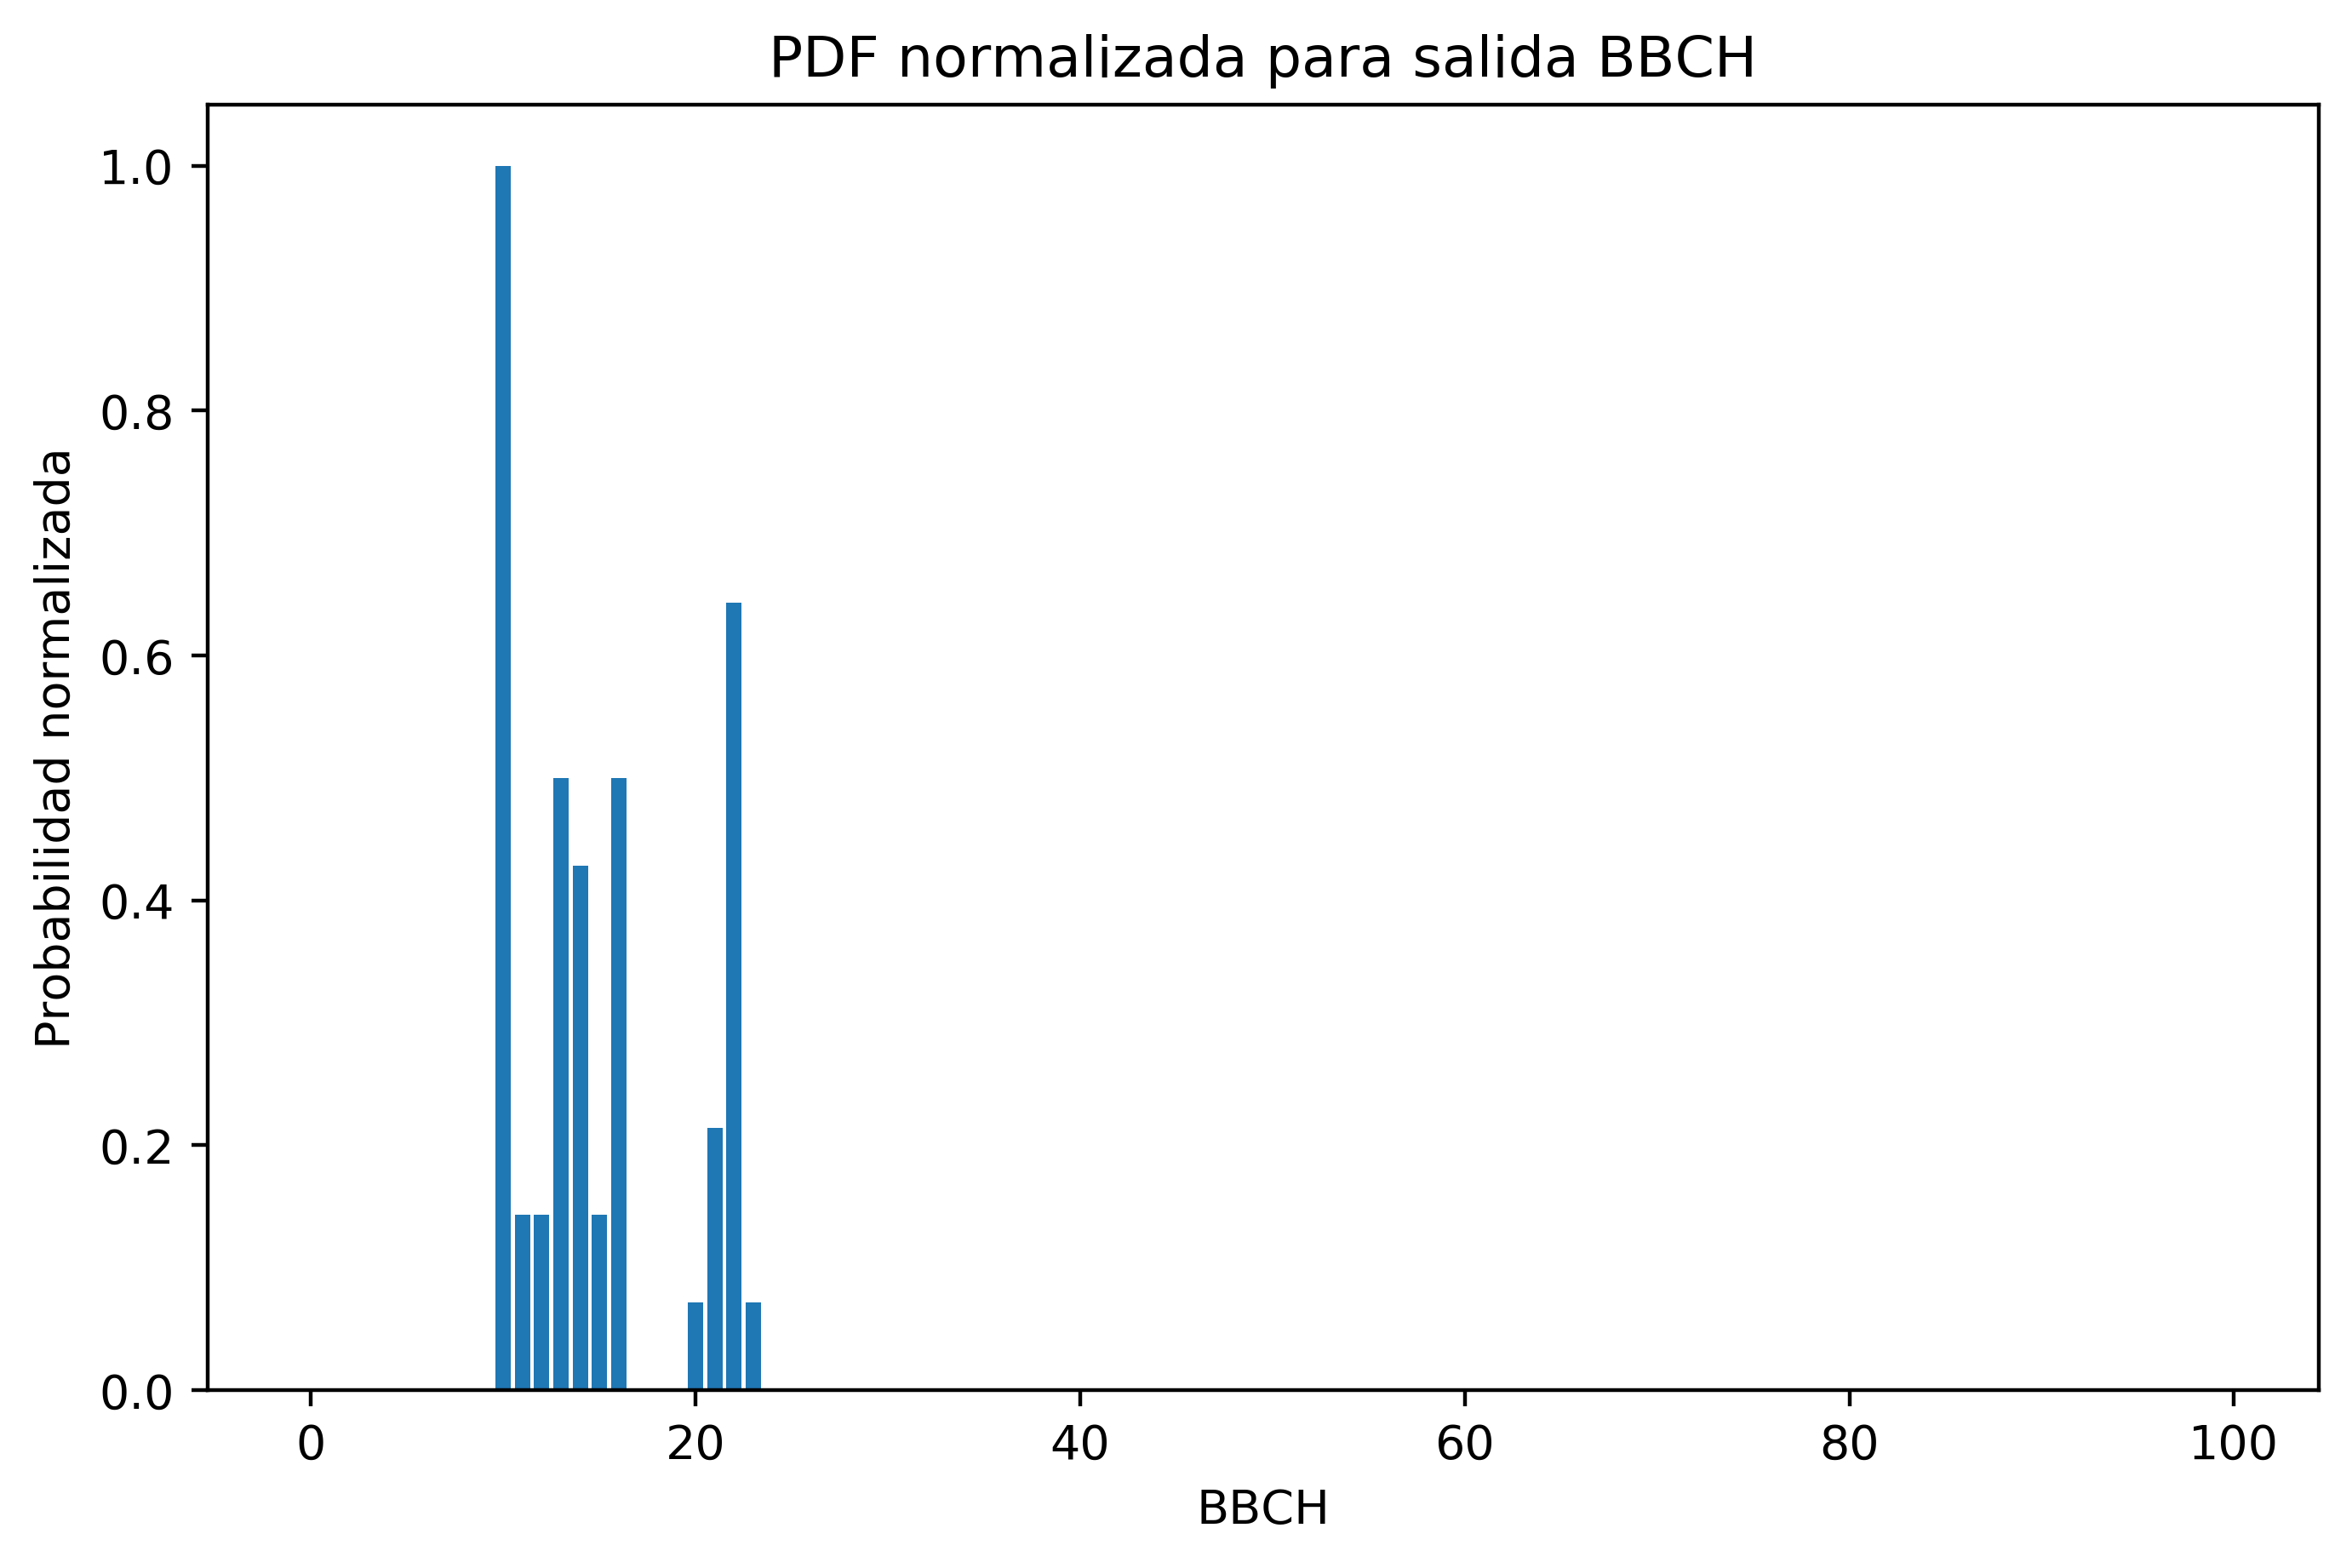
\includegraphics[width=0.95\linewidth]{archivos/tfg/Mean/TEST_PARC_PDF_BH_B}
  \caption{Ejemplo del modelo de doble salida: \gls{pdf} estimación de \gls{bbch}\label{fig:sub1}}
\end{subfigure}
\begin{subfigure}{0.6\textwidth}
  \centering
  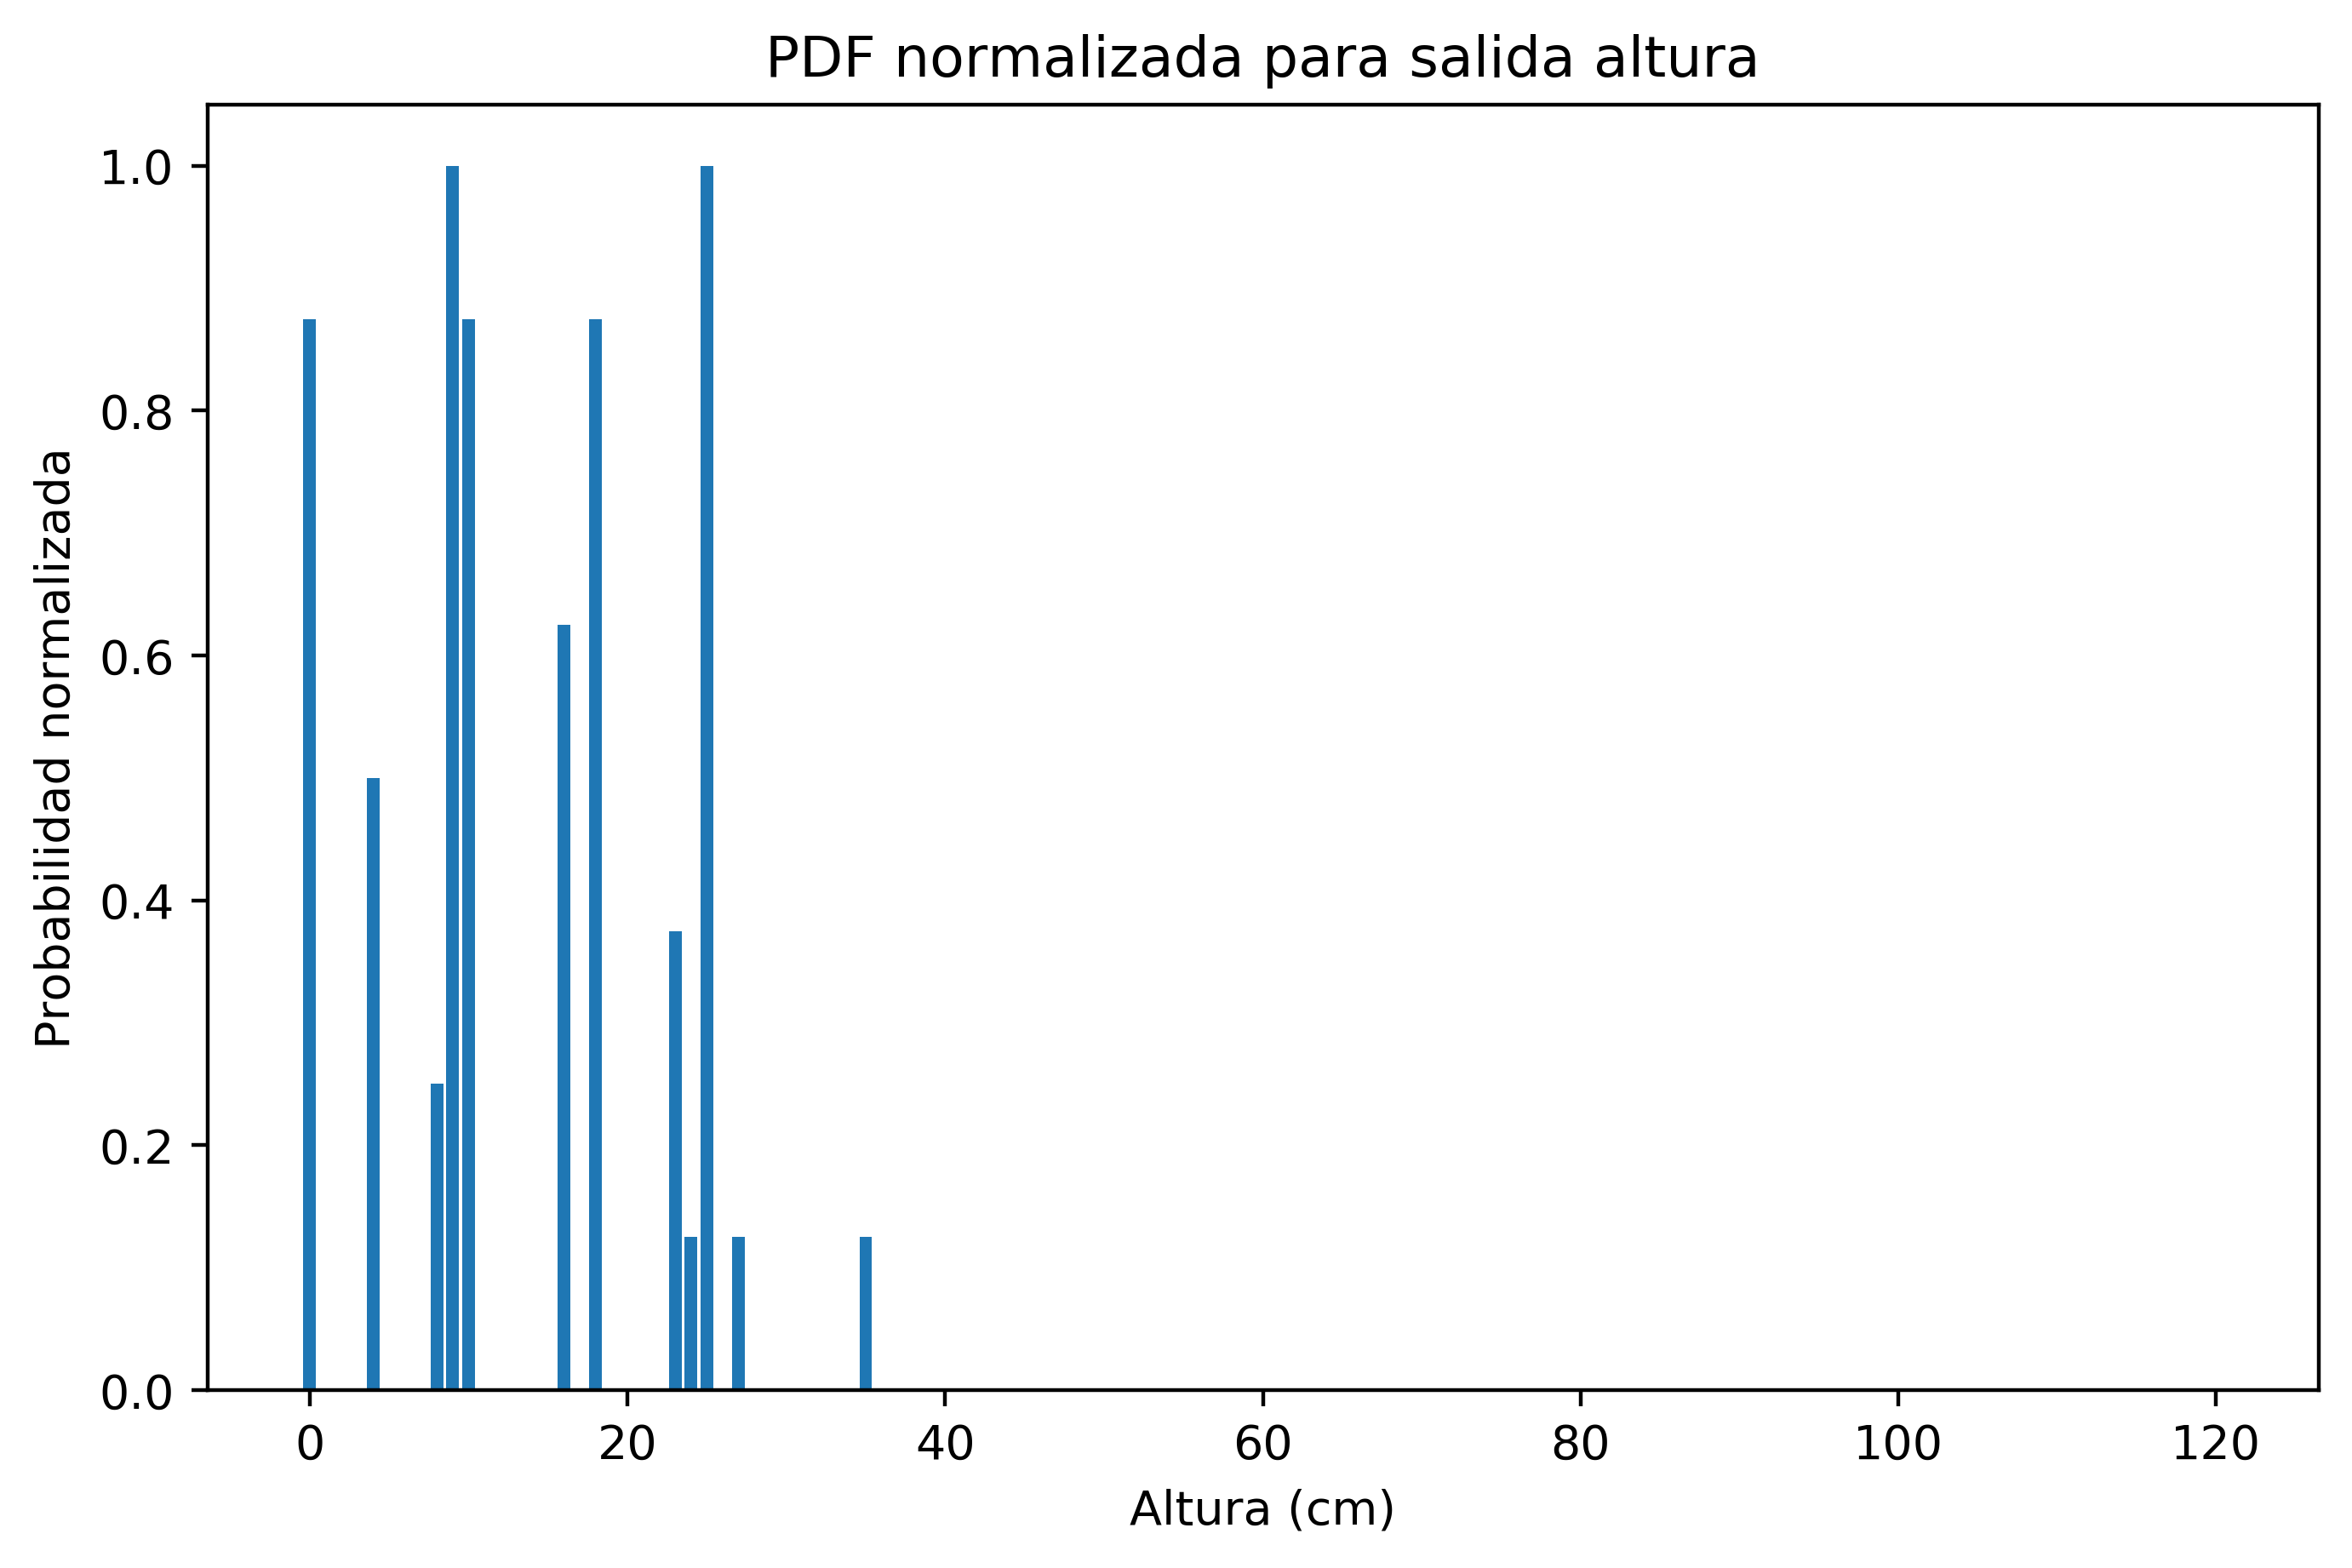
\includegraphics[width=0.95\linewidth]{archivos/tfg/Mean/TEST_PARC_PDF_BH_H}
  \caption{Ejemplo del modelo de doble salida: \gls{pdf} estimación de altura\label{fig:sub2}}
\end{subfigure}
\caption{Ejemplo de salidas \gls{pdf} normalizadas del modelo para estimación de \gls{bbch} y la altura. \label{fig:pdf_bh}}
\end{figure}

\subsubsection{Salidas de valor único}
\par Para continuar con la presentación de los resultados obtenidos, se ilustran en las figuras \ref{fig:comp_b}, \ref{fig:comp_h} y \ref{fig:comp_bh} las comparaciones de las soluciones únicas obtenidas (salida con máxima probabilidad) y los datos de tierra tomados correspondientes para la parcela de test en 2018: \gls{bbch} general, máxima y mínima en la parcela, casos individual (\ref{fig:comp_b}) y de doble salida (\ref{fig:sub_c1}), o la altura general del cultivo, también para ambos casos (figuras \ref{fig:comp_h} y \ref{fig:sub_c2}, respectivamente). Estas salidas, aunque carecen de la información completa, son las más sencillas de comparar y evaluar con los resultados reales, ya que estos también son un único valor.  
\\

% Dos figuras sueltas debajo de otra
\begin{figure}[H]
\centering
\begin{subfigure}{.65\textwidth}
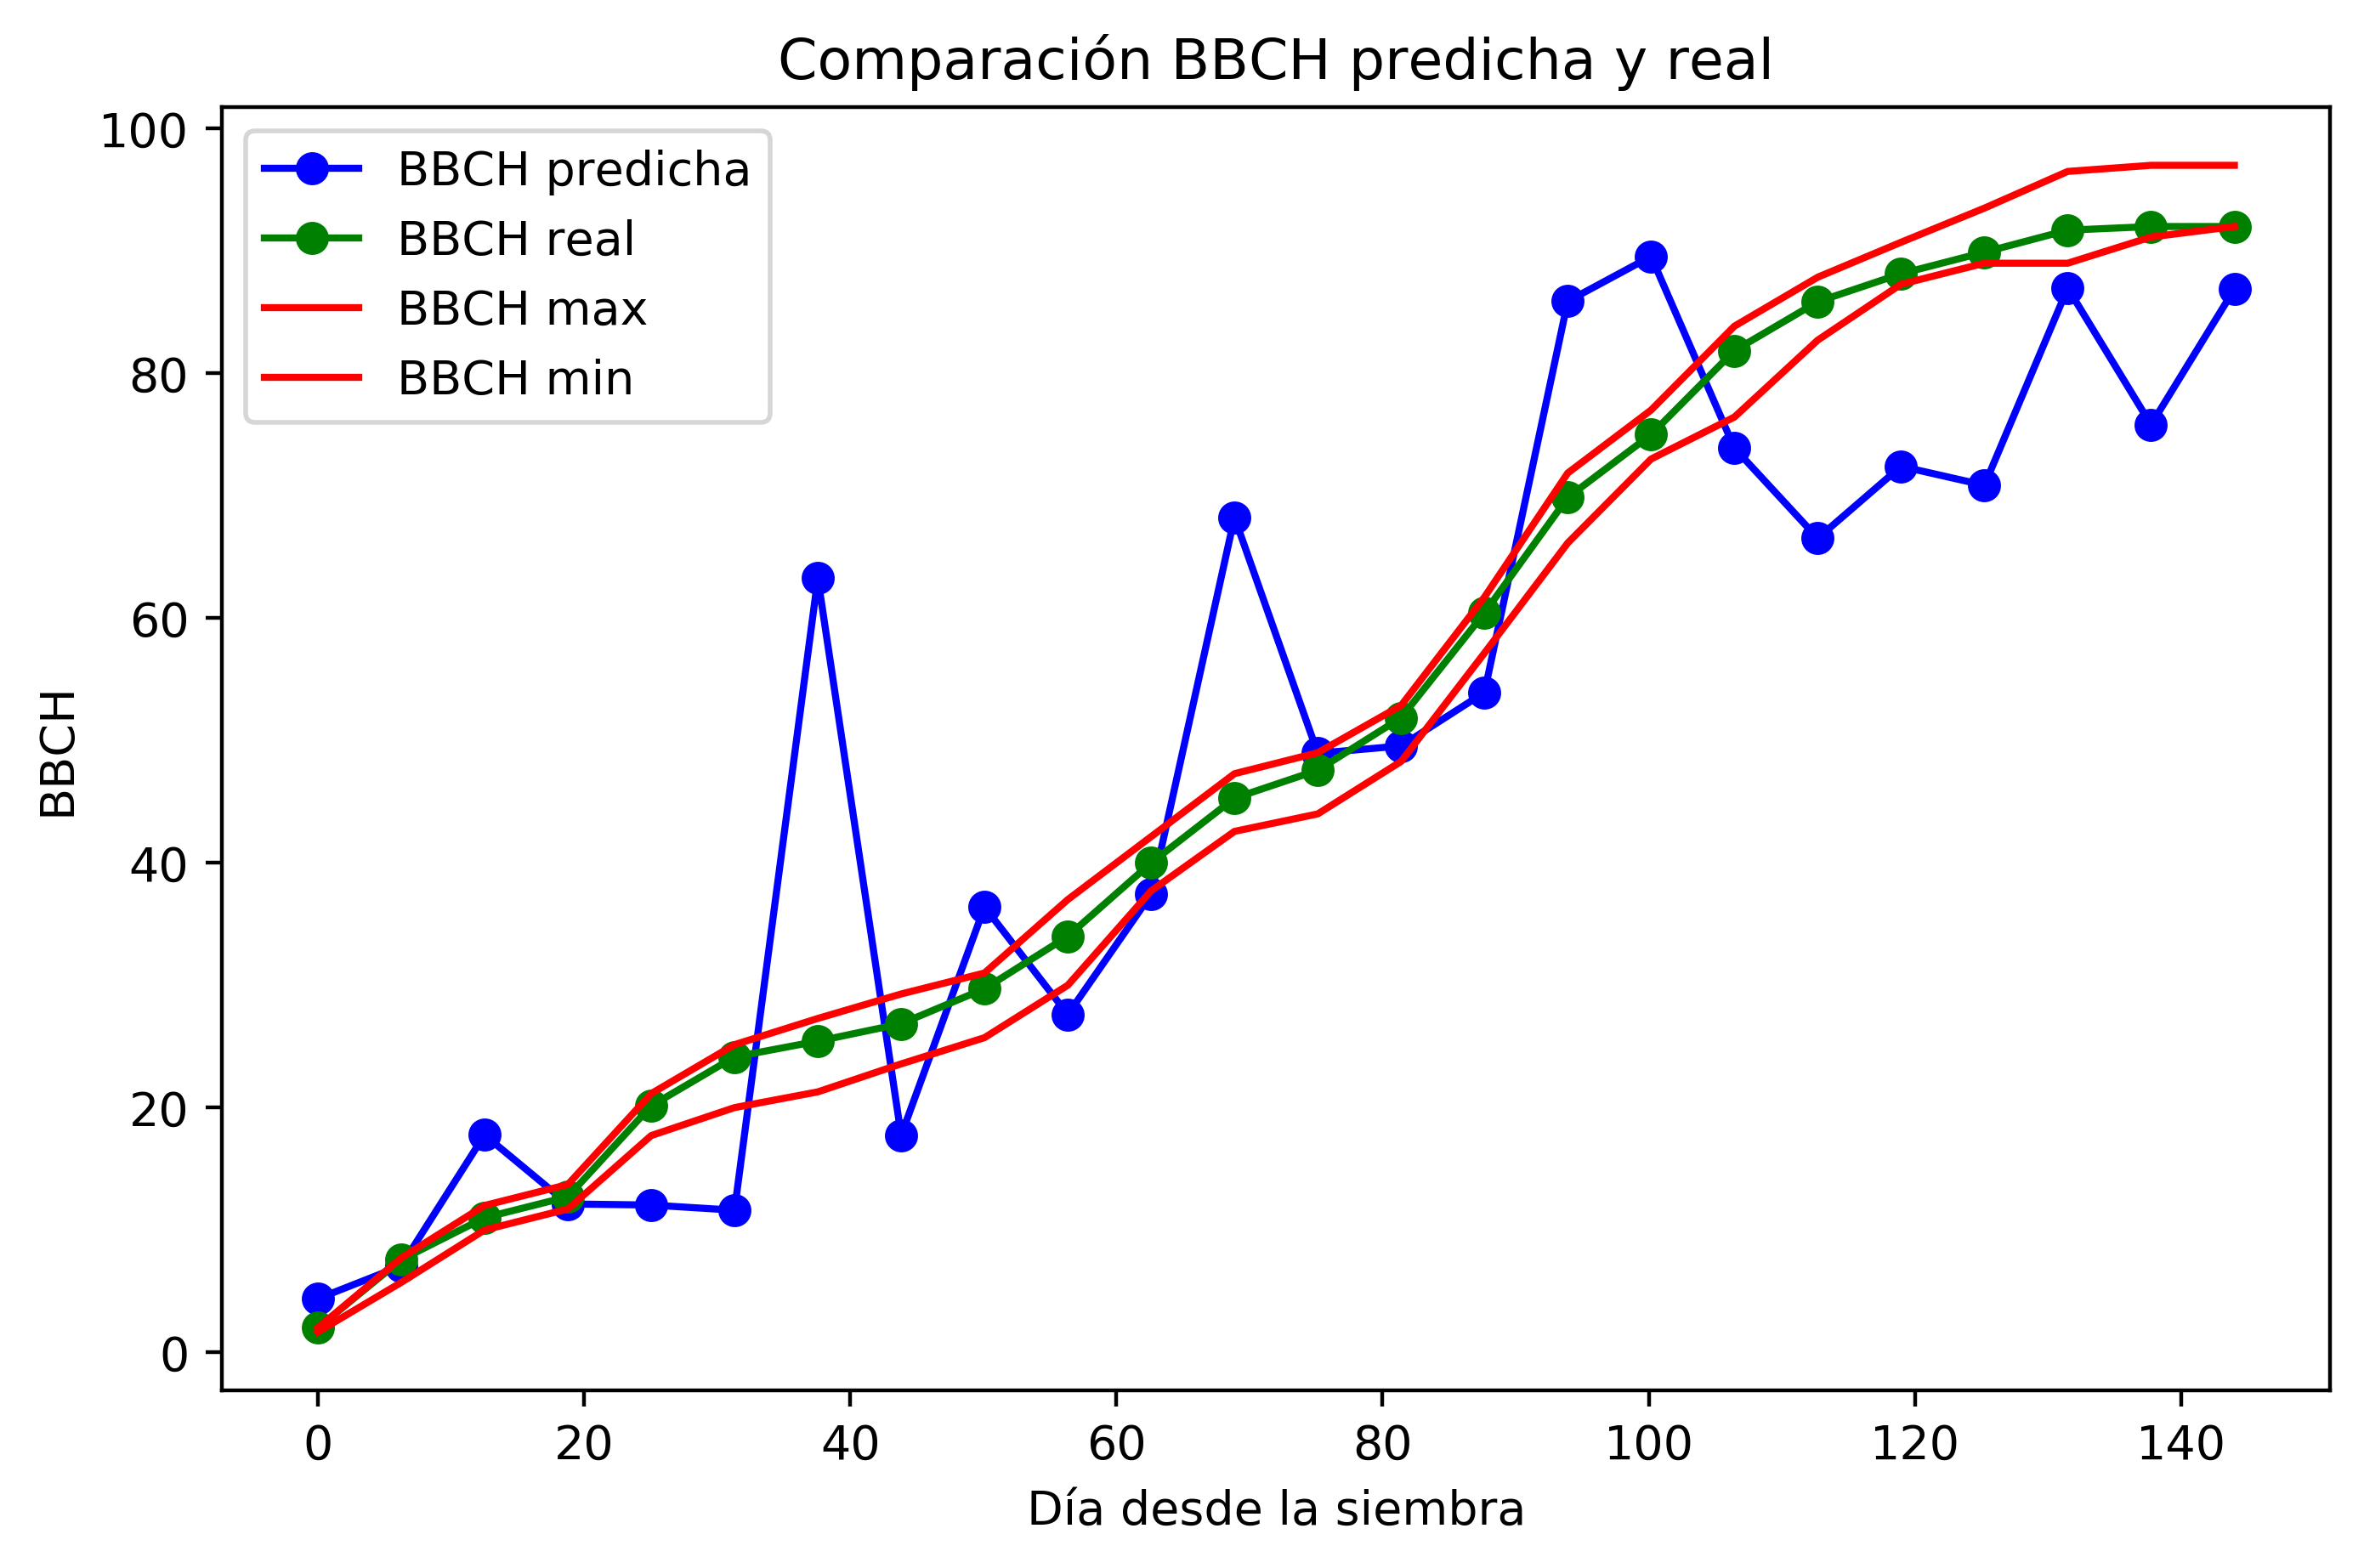
\includegraphics[width=0.95\linewidth]{archivos/tfg/Mean/TEST_PARC_FINAL}
\captionof{figure}{Comparación de la salida predicha y la verdad de tierra del modelo para estimación de \gls{bbch}.\label{fig:comp_b}}
\end{subfigure}
\begin{subfigure}{.65\textwidth}
\centering
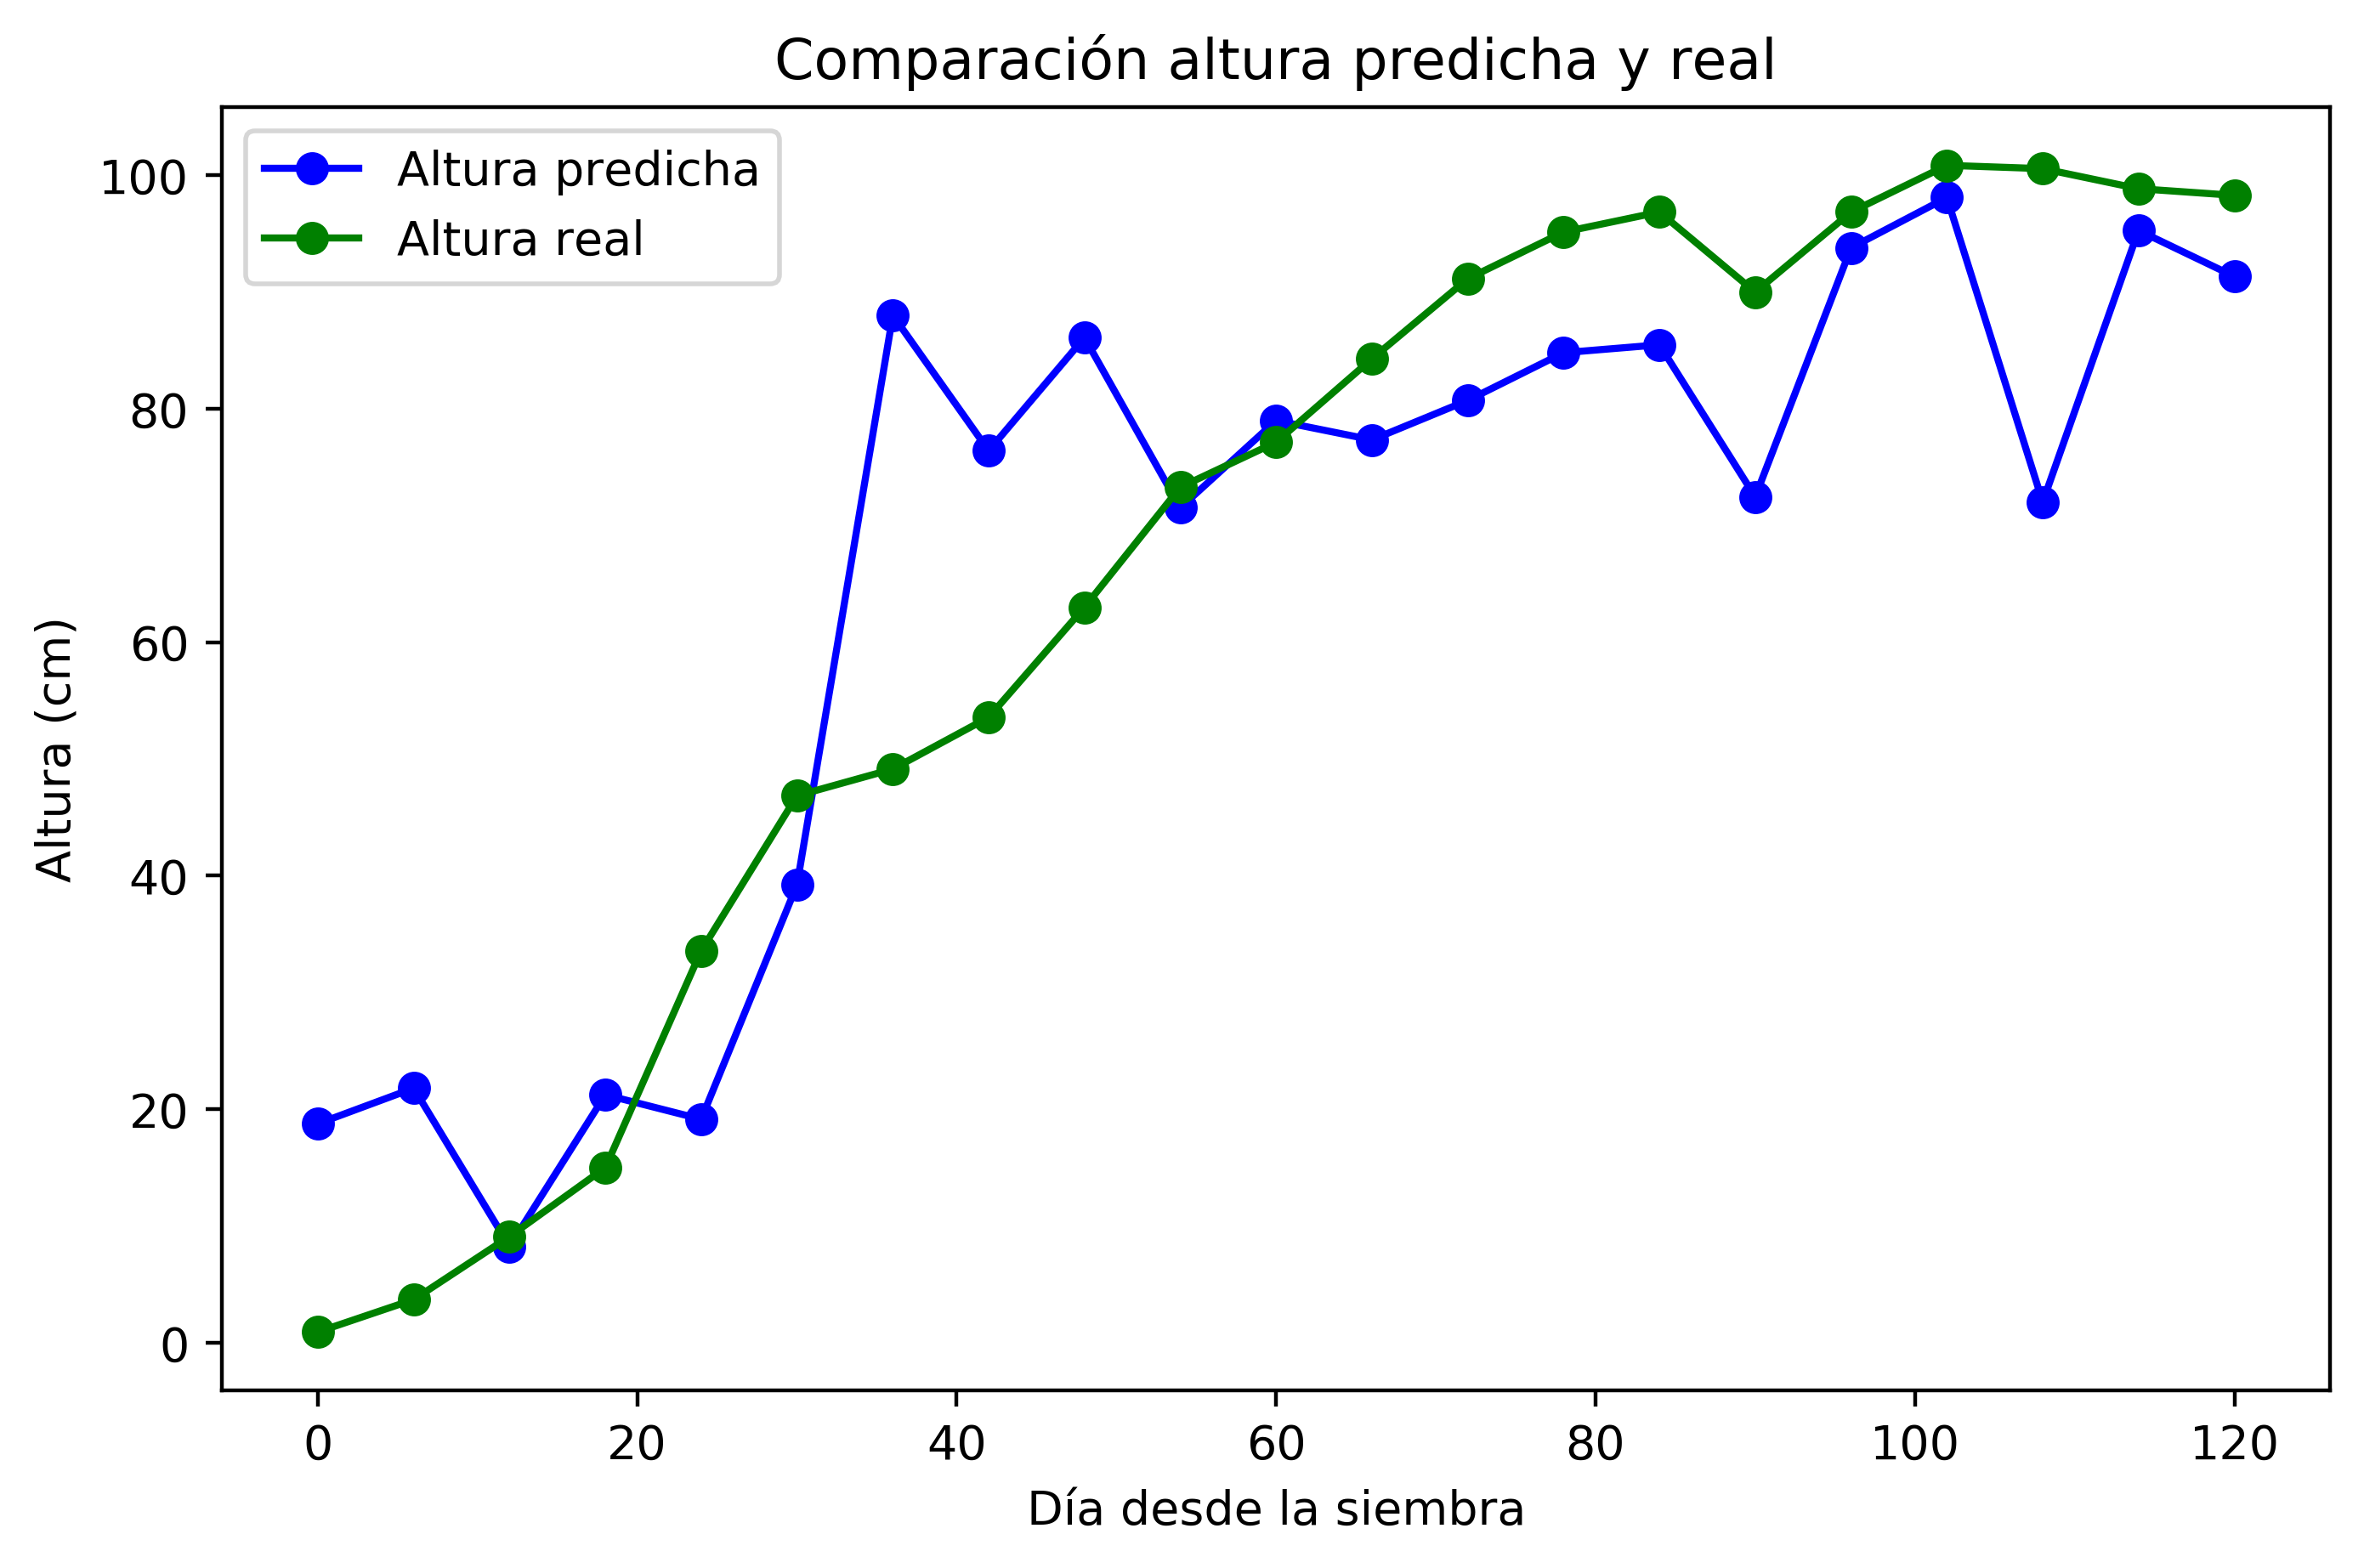
\includegraphics[width=0.95\linewidth]{archivos/tfg/Mean/TEST_PARC_FINAL_H}
\captionof{figure}{Comparación de la salida predicha y la verdad de tierra del modelo para estimación de la altura. \label{fig:comp_h}}
\end{subfigure}
\caption{Comparación de la salida predicha y la verdad de tierra de los modelos de salida individual para la estimación de \gls{bbch} y la altura.}
\end{figure}

\par Comenzando por los modelos de predicción de \gls{bbch} representados en las figuras \ref{fig:comp_b} y \ref{fig:sub_c1}, se pueden observar estimaciones y errores muy parecidos en ambos modelos. Estos son fácilmente comparables ya que la parcela de test coincide para los dos casos. Ambos modelos, presentan estimaciones que, en su mayoría, están fuera de los límites marcados por las líneas de \gls{bbch} máximas y mínimas medidas en campo. En general, se ve una tendencia creciente a lo largo de la variable estimada entorno a los valores reales, aunque con 2 o 3 zonas con picos de error mayor en las que el sistema predice un estado fenológico mayor al real. De hecho, el primer pico en torno a los días 30-40 después de la siembra está presente tanto en la estimación de \gls{bbch} como de la altura en las figuras \ref{fig:comp_h} y \ref{fig:sub_c2}. Teniendo en cuenta que los valores de entrada son iguales para todos los casos, se puede atribuir este fenómeno a anomalías presentes en los datos de satélite, los cuales, en  una etapa concreta del desarrollo del cultivo, pueden presentar valores muy similares a los obtenidos para etapas finales, y por ello cometer un error de predicción bastante grande. Este error sería corregible bien detectando la anomalía y eliminando o modificando esta parte de los datos de entrada, tanto en entrenamiento como en test o futuros usos, o bien comprobando que el modelo está generando predicciones correctas con menor densidad de probabilidad, estando representadas en las salidas de \gls{pdf}, y pudiendo ser consideradas sin un procesamiento extra de los datos, simplemente al contrastarlos con los resultados del modelo temporal, ya que es una diferencia de etapas muy grande y en este modelo no se daría un error de etapa de tal dimensión. 
\\

% Una figura con dos imágenes
\begin{figure}[H]
\centering
\begin{subfigure}{.65\textwidth}
  \centering
  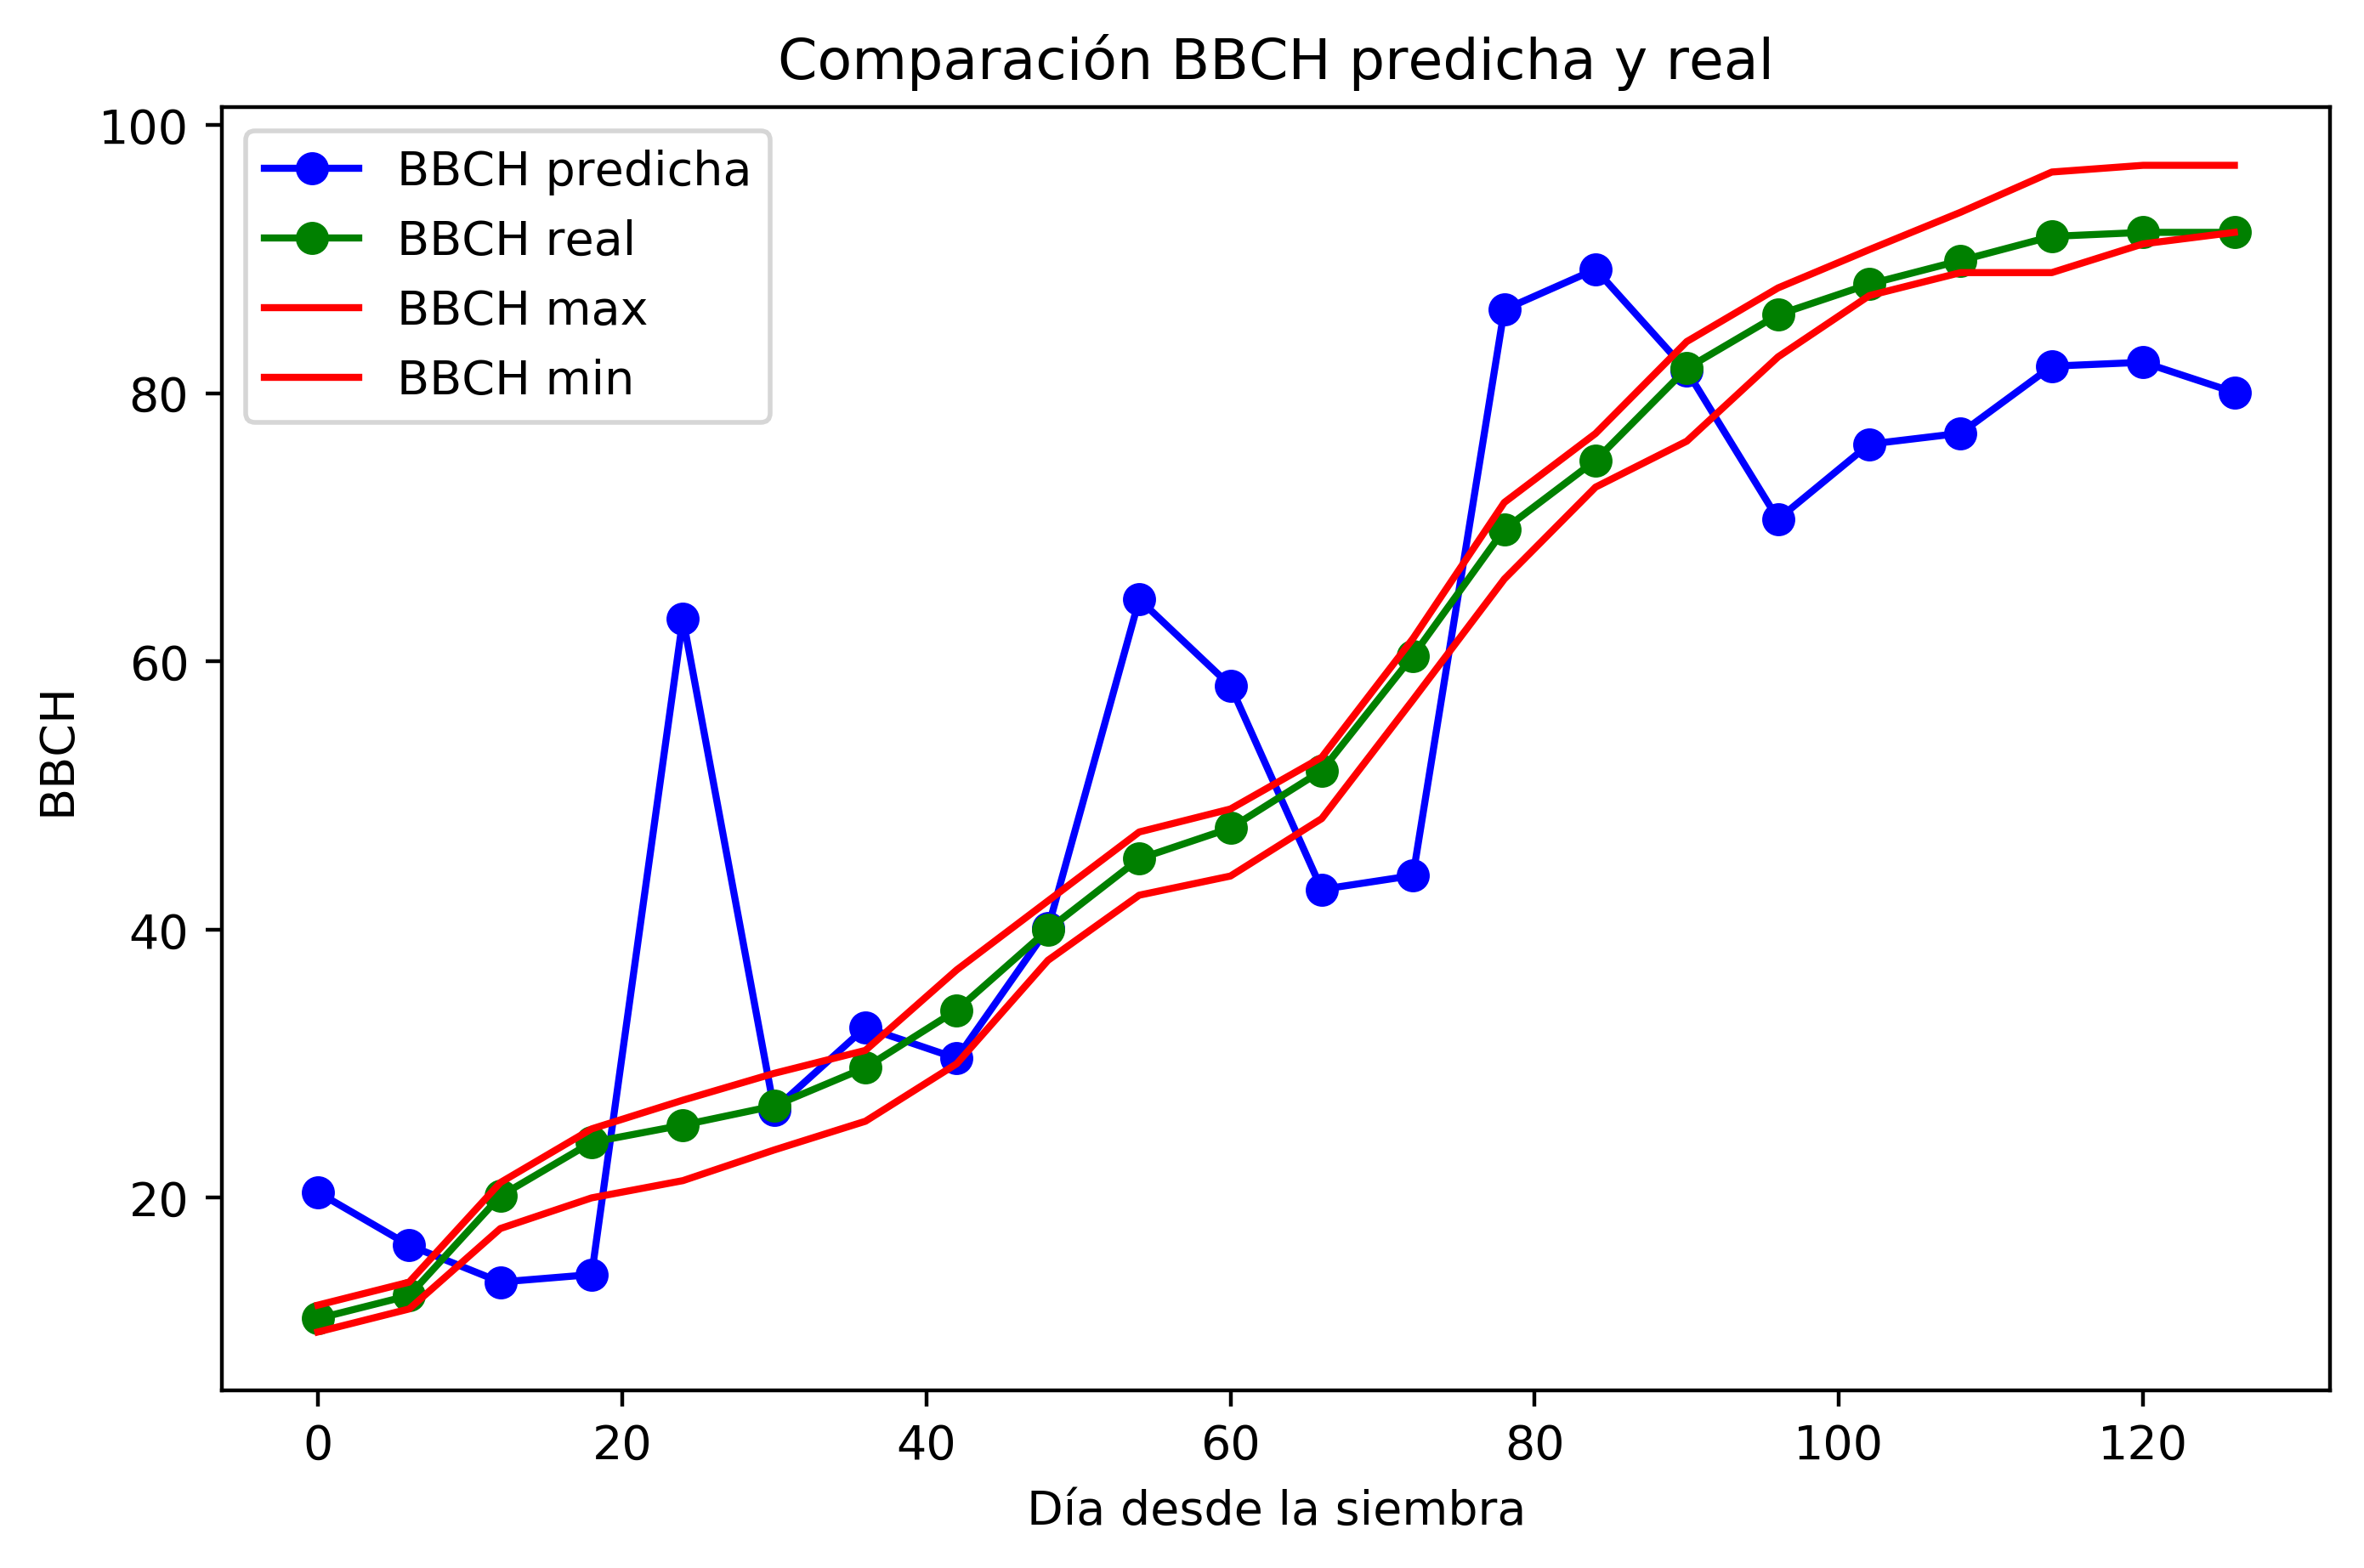
\includegraphics[width=0.95\linewidth]{archivos/tfg/Mean/TEST_PARC_FINAL_BH}
  \caption{Comparación de la salida predicha y la verdad de tierra del modelo de doble salida para la estimación de \gls{bbch}. \label{fig:sub_c1}}
\end{subfigure}
\begin{subfigure}{.65\textwidth}
  \centering
  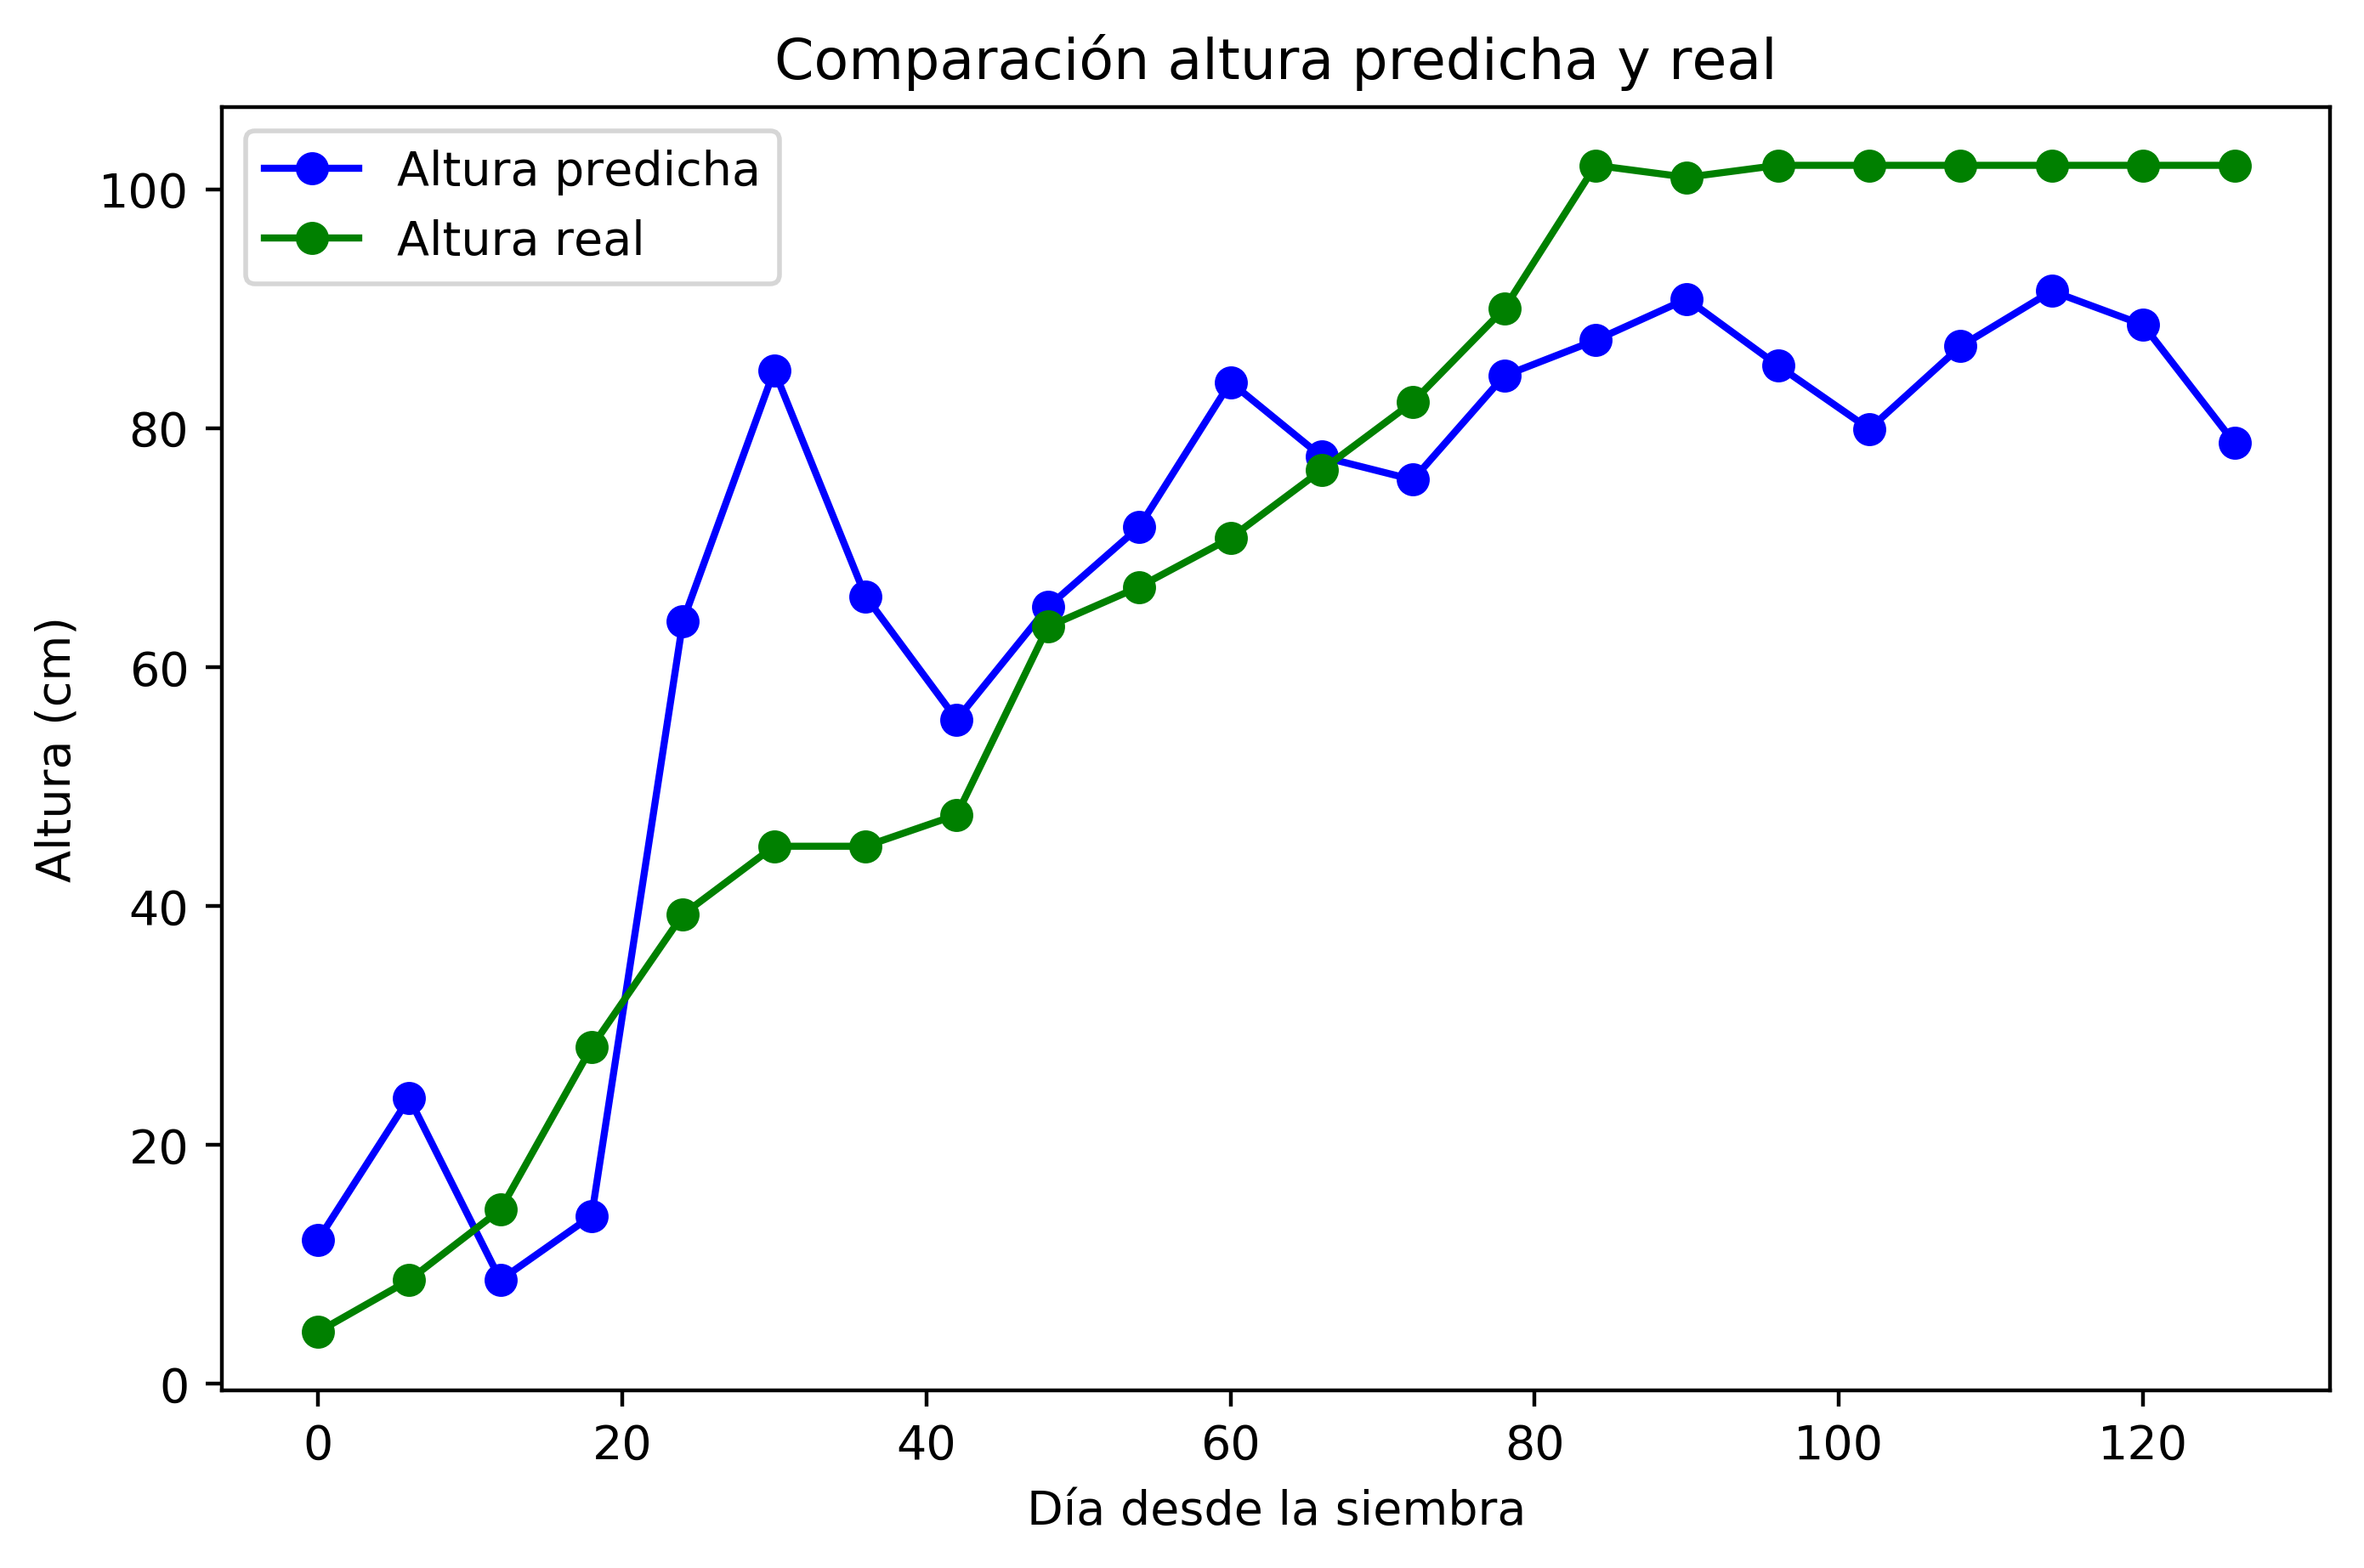
\includegraphics[width=0.95\linewidth]{archivos/tfg/Mean/TEST_PARC_FINAL_BH_H}
  \caption{Comparación de la salida predicha y la verdad de tierra del modelo de doble salida para la estimación de la altura\label{fig:sub_c2}}
\end{subfigure}
\caption{Comparación de la salida predicha y la verdad de tierra del modelo de doble salida para la estimación de \gls{bbch} y la altura. \label{fig:comp_bh}}
\end{figure}

\par Visualizando las salidas para la altura, se puede también comparar, aunque no directamente, el funcionamiento de ambos modelos. En este caso las parcelas de test no son las mismas debido a la optimización para cada modelo, por lo que la comparación simplemente visual entre las dos representaciones es menos intuitiva. Aún así, se aprecian coincidencias como el error en la etapa cercana a 40 días, como se ha mencionado antes, o la estimación de mayor altura para los días de 0 a 10 después de la siembra. En general, ambas representaciones tienen también una tendencia creciente bastante similar a la real, con aparentemente mejor estimación para las etapas finales en el modelo de salida única de altura, ya que en la figura \ref{fig:comp_h} se observa una estimación menor constante para todas las etapas desde el día 80 tras la siembra hasta la cosecha (día 120 aproximadamente).

\subsection{Evaluación de resultados}
\par Para la evaluación de los resultados obtenidos para el método por parcelas se van a utilizar, como se ha mencionado anteriormente, las salidas de valor único por su facilidad para ser representadas y comparadas con los valores únicos medidos. 
\\
\par La primera evaluación realizada se basa en la relación directa entre las salidas estimadas y las medidas reales, lo cuál muestra la fiabilidad del modelo de una forma más clara y así puede verse en las figuras \ref{fig:rel_b}, para el modelo de única salida de \gls{bbch}, \ref{fig:rel_h}, para el modelo de única salida de altura y la figura \ref{fig:rel_bh} para el modelo de doble salida. En estas representaciones se añade, además, una recta de pendiente ($m$) unidad, la cual sirve de referencia ya que esa relación representaría un modelo ideal. Se han utilizado para todas las representaciones los valores contrastados de la parcela de test correspondiente a cada caso, teniendo en cuenta ambos años de datos, 2017 y 2018.

\par En la figura \ref{fig:rel_b} se aprecia una distribución uniforme, lo cuál indica que se disponen de datos suficientes para cubrir las distintas etapas del desarrollo del cultivo. Además, las nubes de puntos se mantienen, en general, cercanos a la recta de referencia, por lo que, excepto para puntos concretos como el pico de las etapas tempranas y las últimas etapas del cultivo, se obtienen resultados bastante buenos. Comparando esta información con la obtenida para el modelo de dos salidas, representado en la figura \ref{fig:rel_bh_b}, se puede asegurar a simple vista qué modelo da mejores resultados. En esta última figura las nubes de puntos se presentan más dispersas que en el anterior, aunque siguiendo la tendencia de la recta de referencia. Vemos, contrariamente, agrupaciones de puntos y huecos, por lo que algunas etapas no están siendo estimadas correctamente. Esto se puede deber al hecho de que el procesamiento de este modelo incluye una etapa de limpieza de datos corruptos que se encuentran en los datos de altura, por lo que en algunas etapas, tanto para la \gls{bbch} como  para la altura, faltan datos que aporten la información completa al sistema. 
\\
\par Comparando a continuación las figuras de los modelos con salida de altura del cultivo, \ref{fig:rel_bh} para salida única y \ref{fig:rel_bh_h} para salida doble, se observa en ambos una mayor inestabilidad en general debida a la concentración de puntos en algunas etapas. La altura de los cultivos no tiene un crecimiento tan lineal progresivo como la fenología de un cultivo, por lo que, a parte de por la corrección de datos, se encuentran concentraciones de datos debido a la estabilidad de la altura durante distintas etapas. Es por ello que, sobre todo en las etapas finales, hay una mayor concentración de puntos, cuando el arroz se mantiene en altura. Aún así, en la figura \ref{fig:rel_bh} se aprecia que todas las estimaciones de altura tienden a la baja para casi todos los datos de altura mayor a 80cm. Una posible explicación sería una tendencia generalizada más baja en las parcelas utilizadas para entrenar el modelo o la poca variación en los parámetros de entrada para alturas desde 50cm hasta 110cm, intervalo en el que la altura estimada se mantiene en torno a la misma franja de valores. 

% Dos figuras sueltas debajo de otra
\begin{figure}[H]
\centering
\begin{subfigure}{0.8\textwidth}
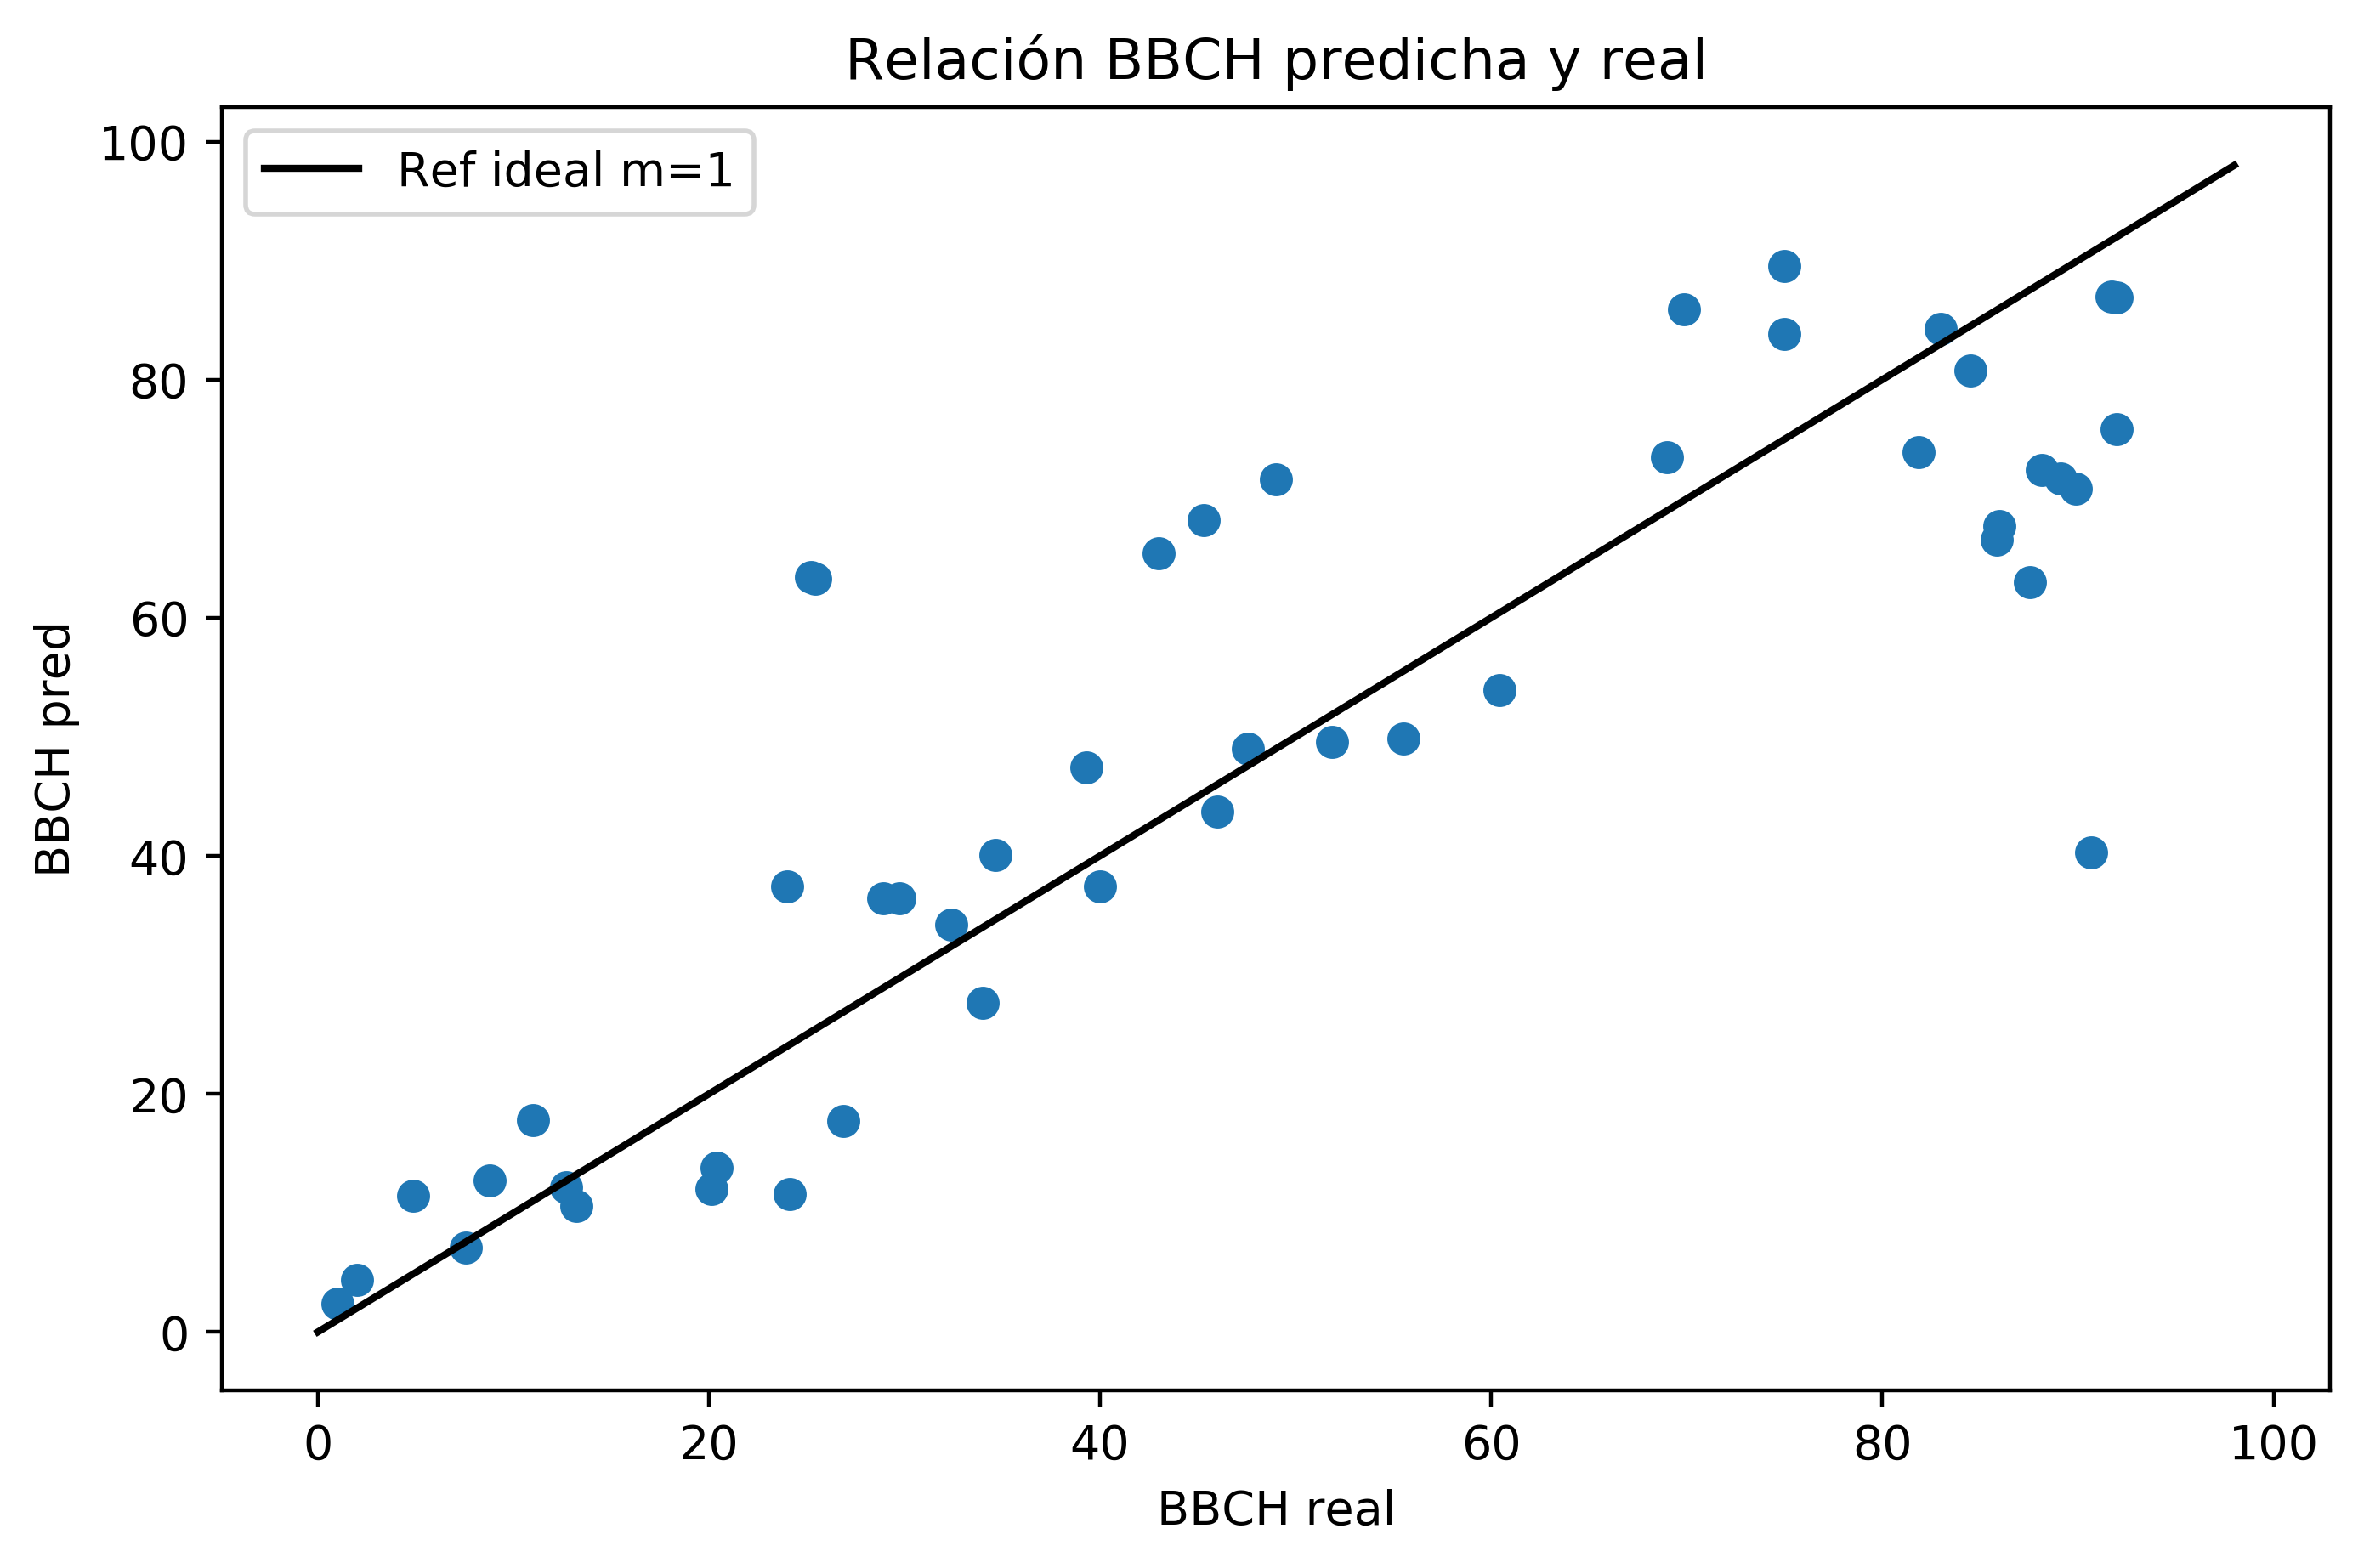
\includegraphics[width=0.95\linewidth]{archivos/tfg/Mean/TEST_PARC_RECTA}
\caption{Relación de la salida predicha y la verdad de tierra del modelo para estimación de \gls{bbch}.\label{fig:rel_b}}
\end{subfigure}
\begin{subfigure}{.8\textwidth}
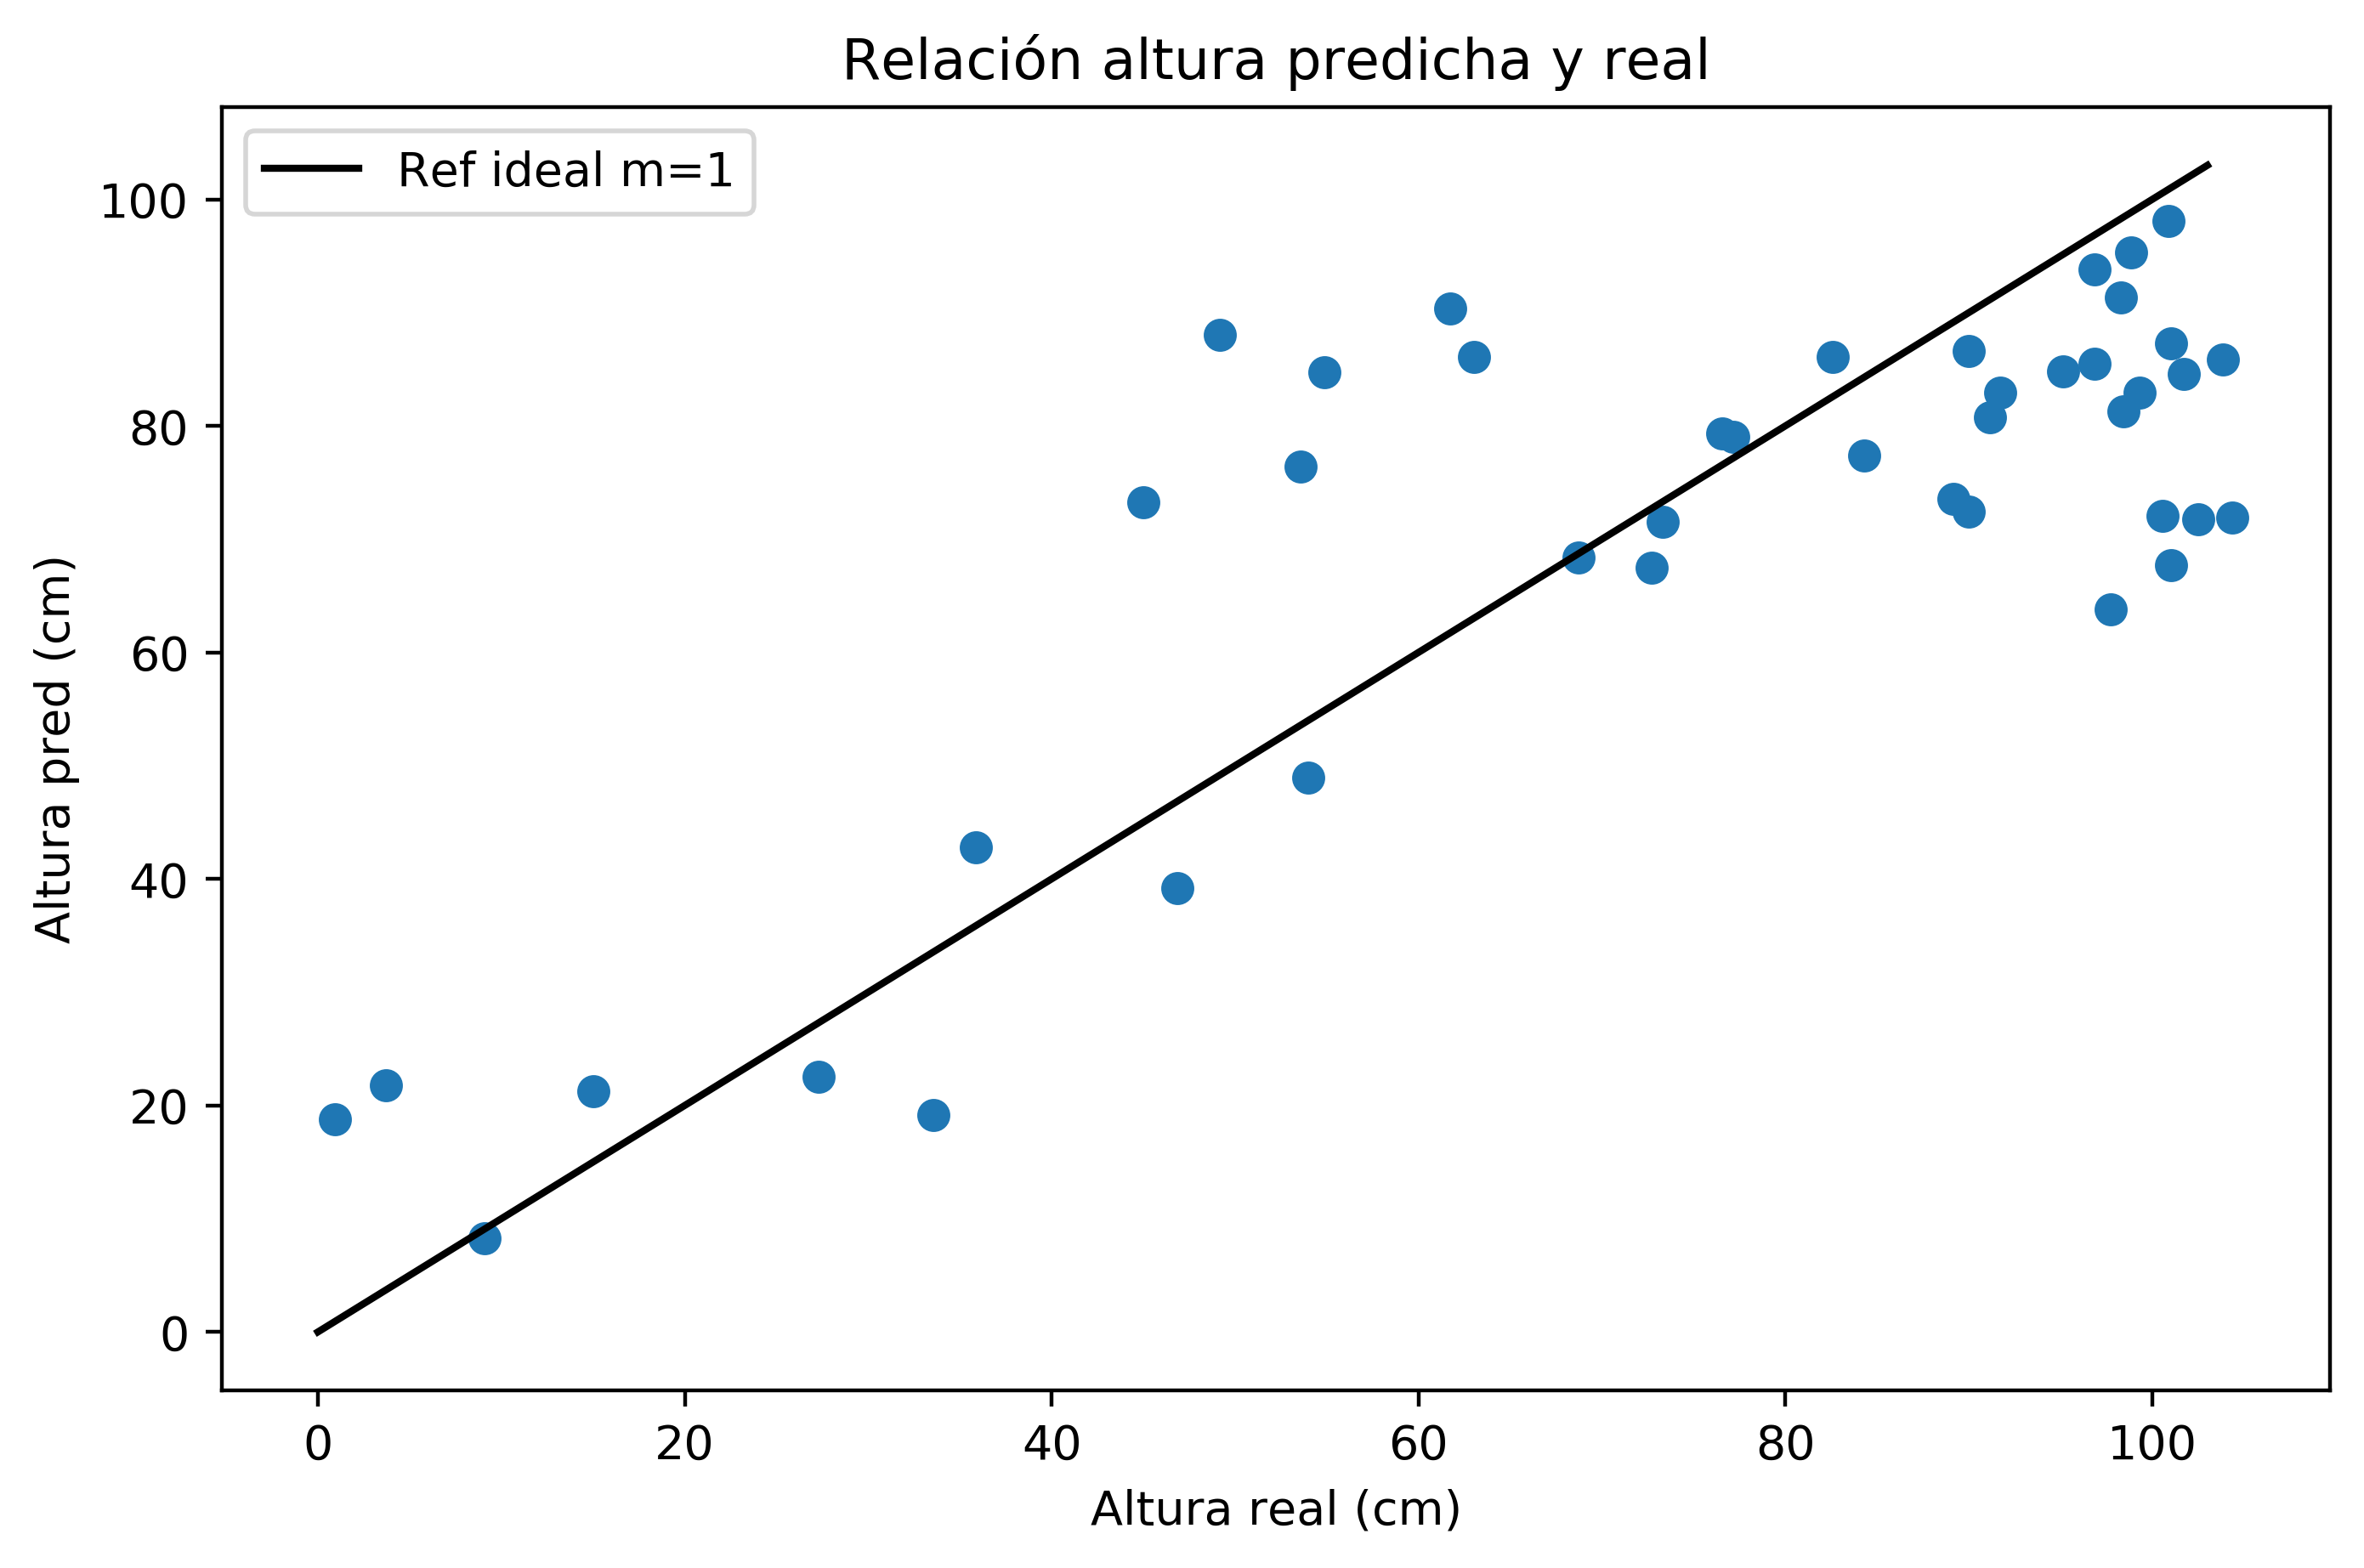
\includegraphics[width=0.95\linewidth]{archivos/tfg/Mean/TEST_PARC_RECTA_H}
\caption{Relación de la salida predicha y la verdad de tierra del modelo para estimación de la altura. \label{fig:rel_h}}
\end{subfigure}
\caption{Relación de la salida predicha y la verdad de tierra de los modelos de variables independientes. \label{fig:rel}}
\end{figure}

% Una figura con dos imágenes
\begin{figure}[H]
\centering
\begin{subfigure}{.8\textwidth}
  \centering
  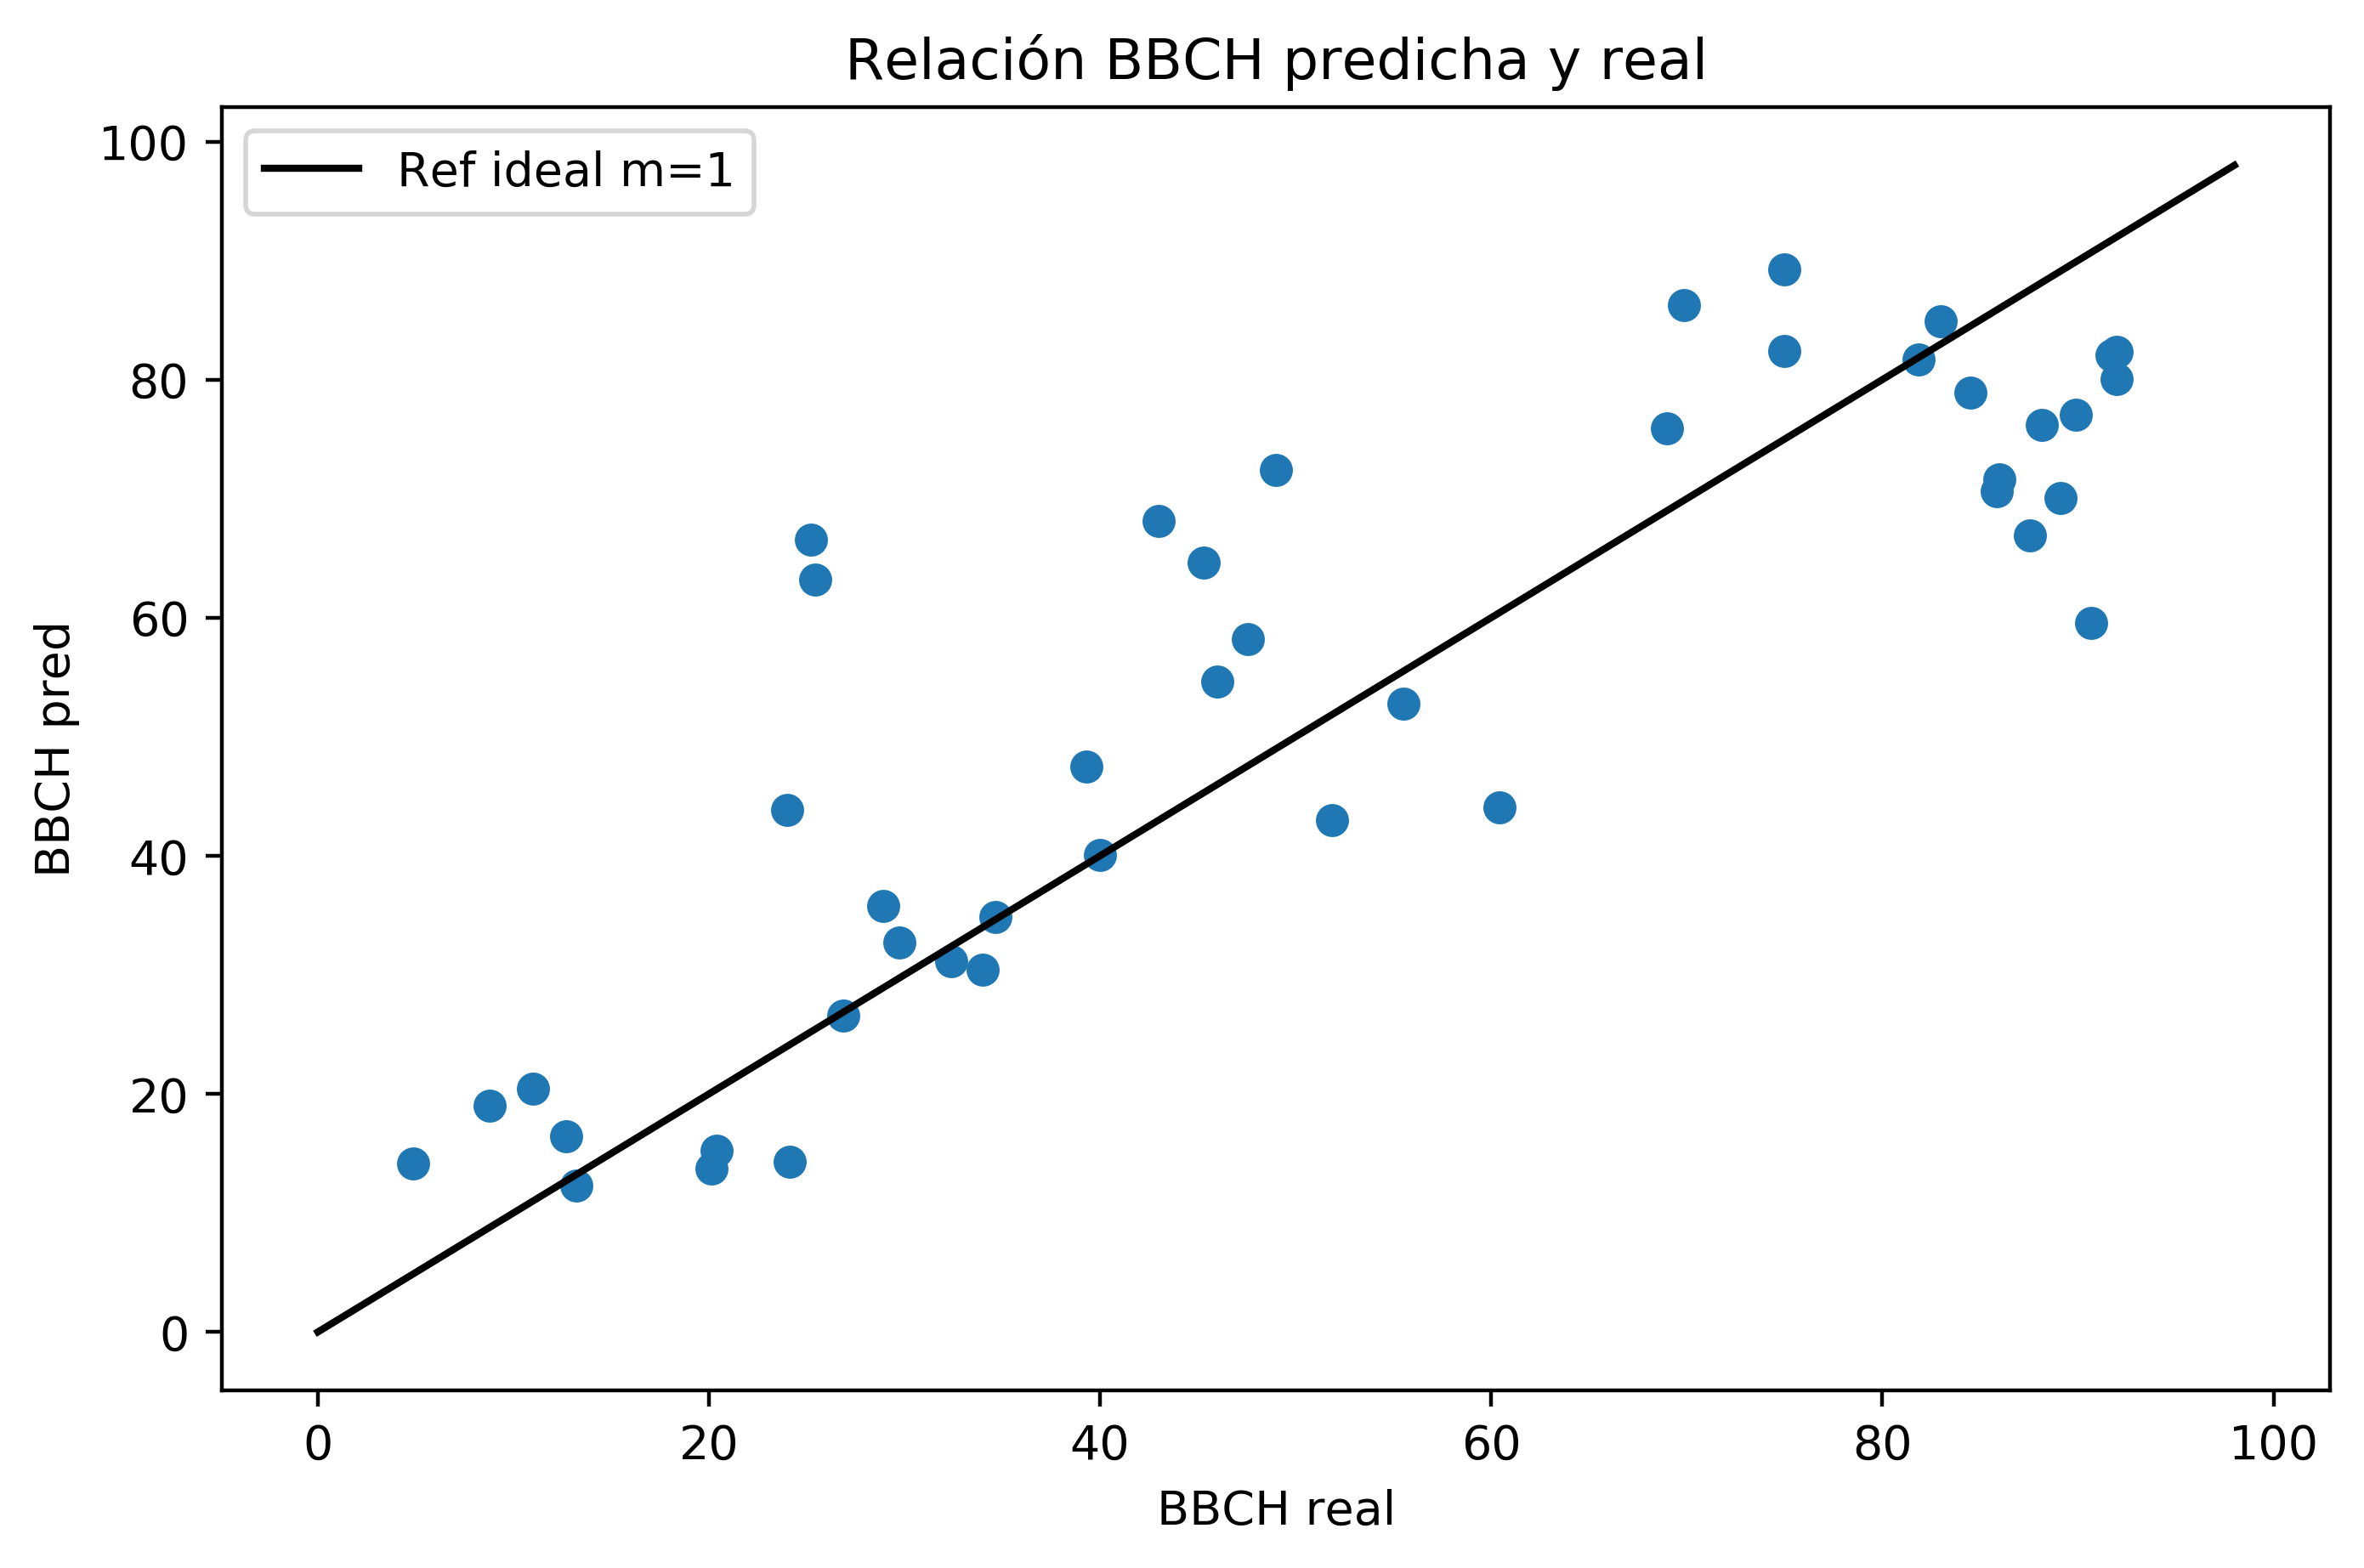
\includegraphics[width=0.95\linewidth]{archivos/tfg/Mean/TEST_PARC_RECTA_bh}
  \caption{Relación de la salida predicha y la verdad de tierra del modelo de doble salida para la estimación de \gls{bbch}. \label{fig:rel_bh_b}}
\end{subfigure}
\begin{subfigure}{.8\textwidth}
  \centering
  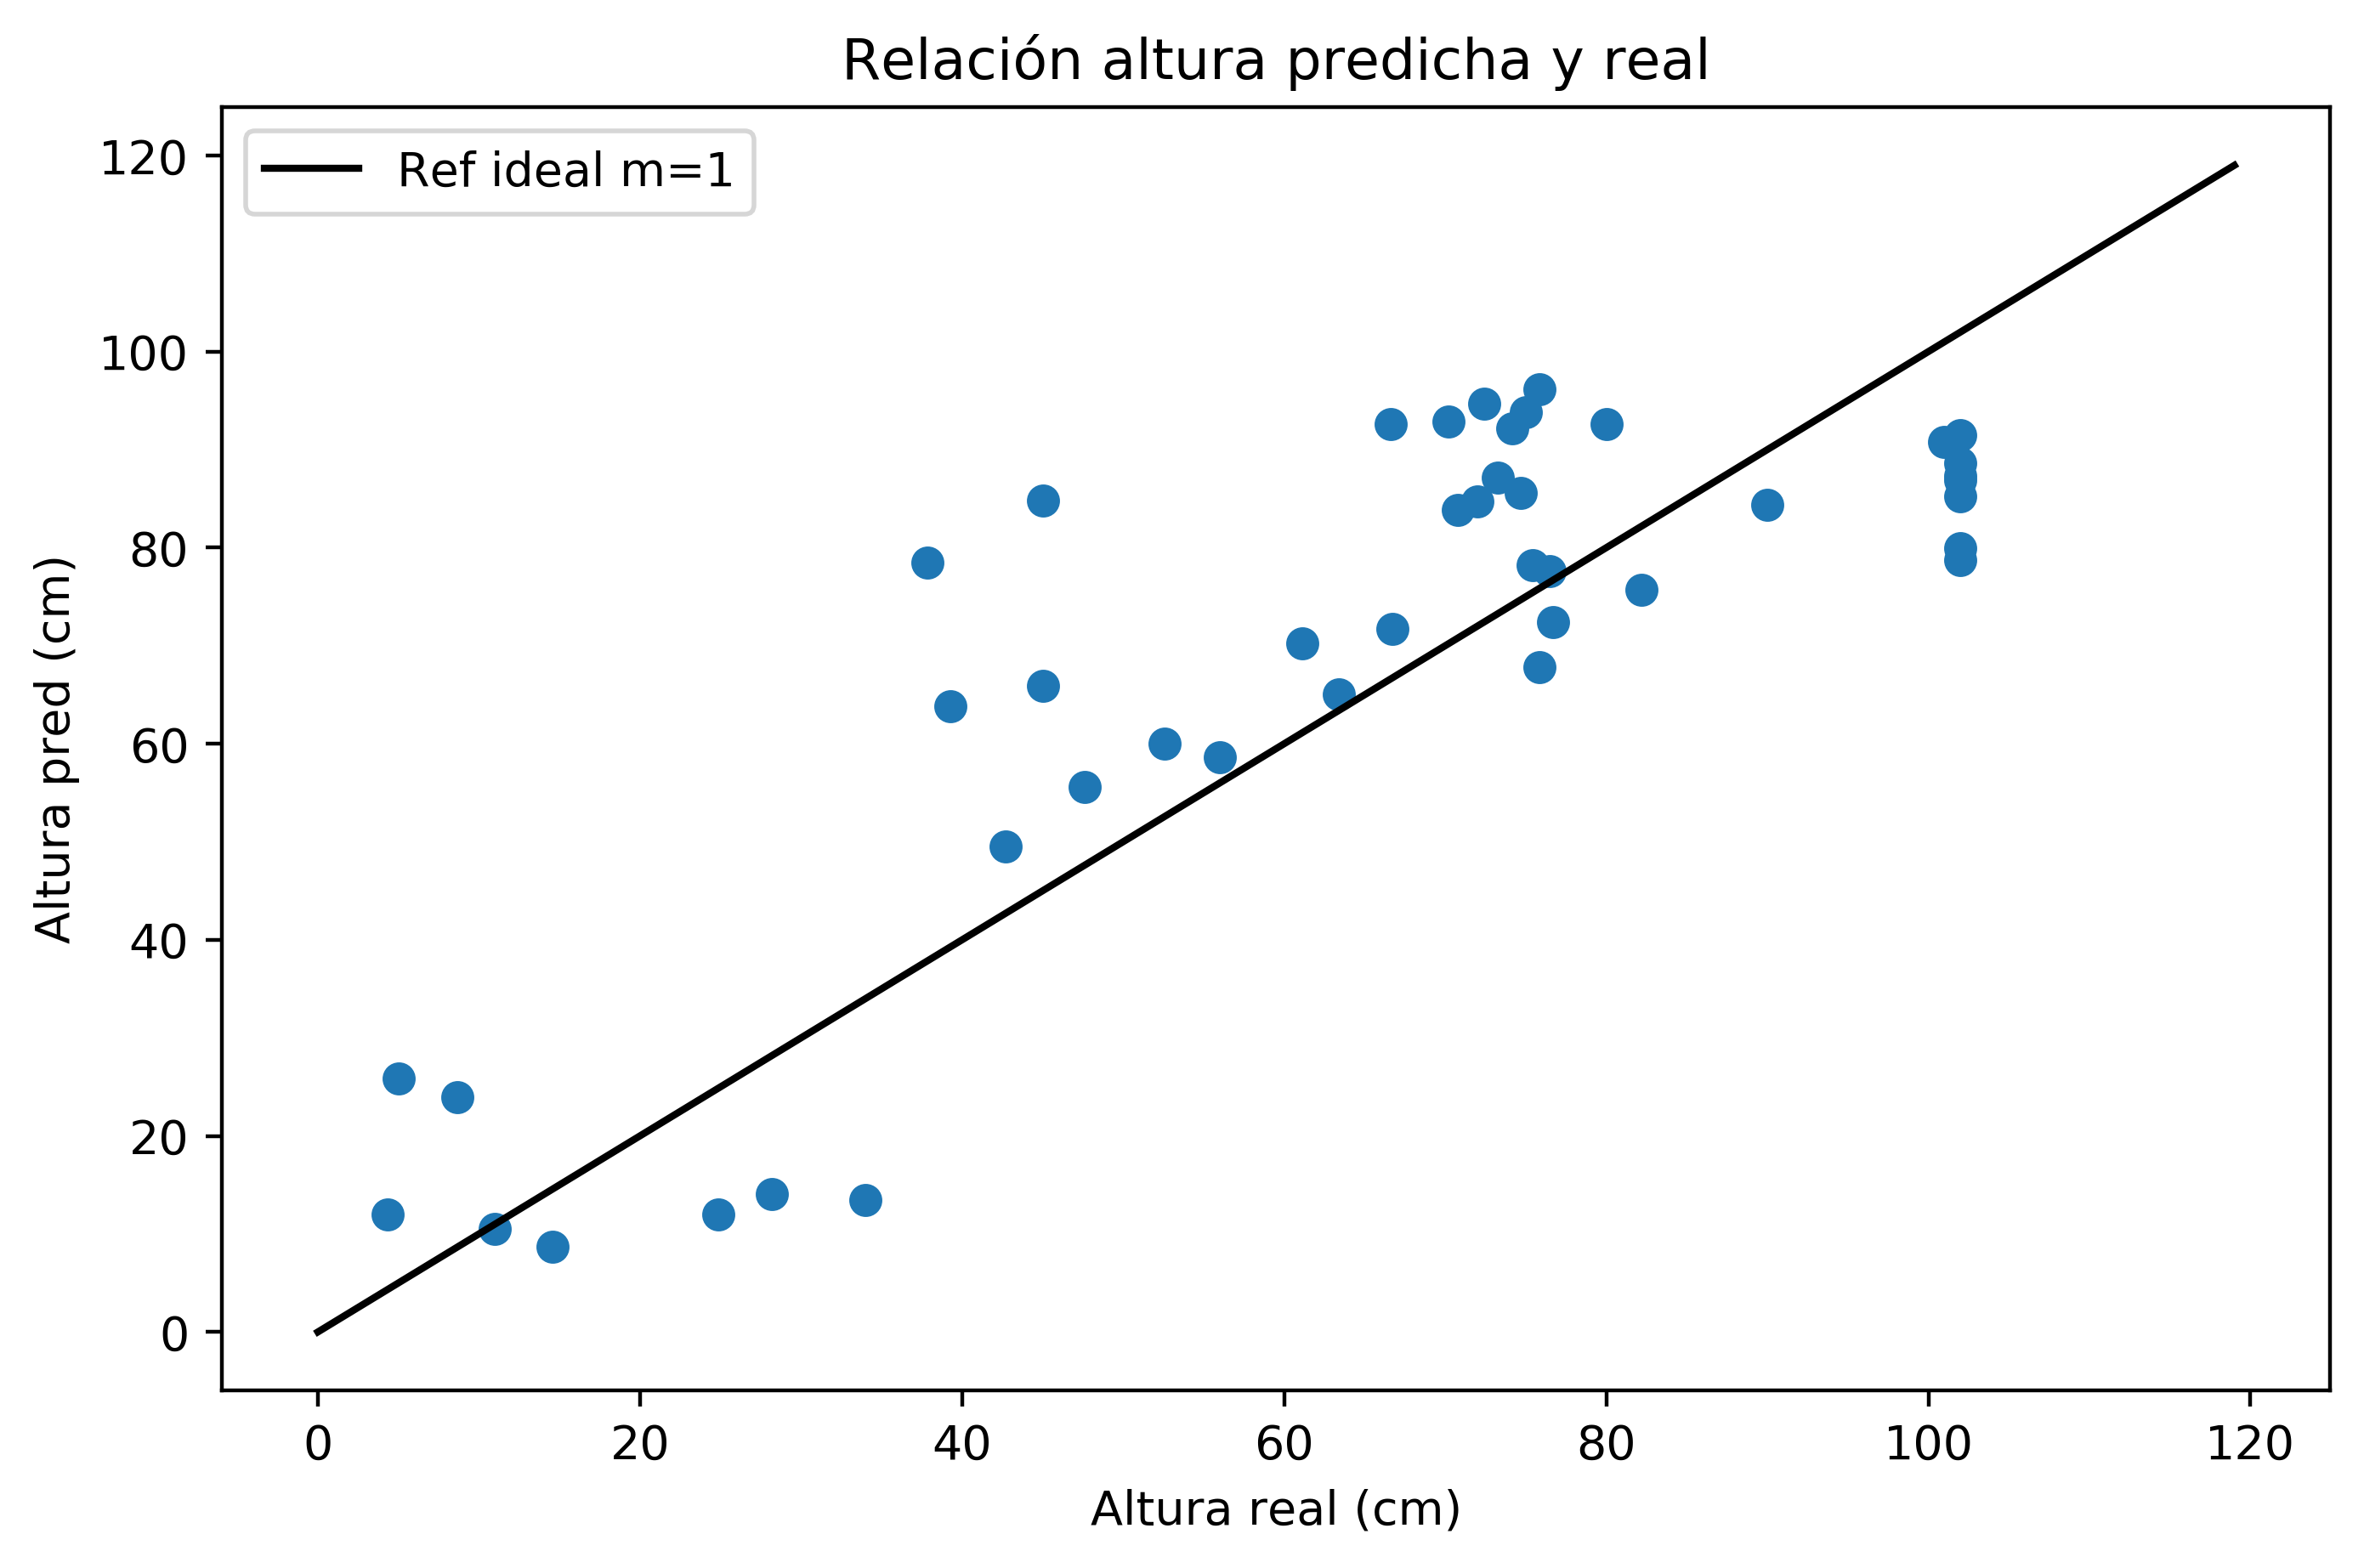
\includegraphics[width=0.95\linewidth]{archivos/tfg/Mean/TEST_PARC_RECTA_bh_H}
  \caption{Relación de la salida predicha y la verdad de tierra del modelo de doble salida para la estimación de la altura\label{fig:rel_bh_h}}
\end{subfigure}
\caption{Relación de la salida predicha y la verdad de tierra del modelo de doble salida para la estimación de \gls{bbch} y la altura. \label{fig:rel_bh}}
\end{figure}

\par A parte de la evaluación con descriptores estadísticos que se realizan a la hora de comparar los dos métodos, se realiza también una evaluación de los datos de entrada utilizados. La tabla \ref{tab:imp_f} representa el peso que tiene cada una de las variables de entrada en el modelo generado para cada uno de los 3 casos tratados. 
\\
\begin{table}[h] 
\centering
\begin{tabular}{l|ccc}
               & \gls{bbch} & Altura & \gls{bbch}\&Altura \\ \hline \hline
VV             & 0.12 & 0.12   & 0.12         \\
VH             & 0.52 & 0.52   & 0.53         \\
Ratio VH/VV    & 0.11 & 0.11   & 0.10         \\
Dev est. VV    & 0.09 & 0.09   & 0.10         \\
Dev est. VH    & 0.07 & 0.09   & 0.09         \\
Dev est. ratio & 0.07 & 0.07   & 0.06        
\end{tabular}
\caption{Influencia de los parámetros de entrada en el modelo de estimación.\label{tab:imp_f}}
\end{table}

\par En la tabla \ref{tab:imp_f} se presentan proporciones altamente similares para los 3 casos contemplados, siendo incluso idénticos para los modelos de salidas independientes. El parámetro de entrada que destaca principalmente sobre el resto es el coeficiente de backscattering para la polarización VH, con más del 50\% de la predicción elaborada en base a él. Los siguientes parámetros más influyentes son el coeficiente de backscattering para la polarización VV y el ratio de ambos, y, por último, las desviaciones estándar, que suponen menos del 10\% de la predicción final. Para comprender mejor porqué existen estas diferencias, se representan en la figura \ref{fig:rel_param} la relación entre cada una de las variables con \gls{bbch}.
\\
\par Lo primero que se observa en la figura \ref{fig:rel_param} es que todas las subfiguras, en general, presentan una tendencia creciente conforme \gls{bbch} va creciendo, que a los primeros estados corresponden valores más bajos y que en todas aparece el pico de detección entorno a un valor de \gls{bbch} de 20-30, que se asemeja a los valores obtenidos por los mismos parámetros para \gls{bbch} cercanas a la cosecha. Esto confirma que las predicciones erróneas cercanas a estas etapas vienen dadas por esta anomalía a la que se le podría buscar corrección. 
\\
\par Comparando los valores que se obtienen para los distintos parámetros a partir de una \gls{bbch} de 40, se aprecia en la subfigura \ref{fig:VH} que su evolución es la más estable y además creciente. Esto quiere decir que, al contrario que en las subfiguras \ref{fig:VV} y \ref{fig:RATIO}, no hay oscilaciones en los valores de entrada y, por tanto, la predicción a partir de estos valores es más sencilla que si para un mismo valor de entrada pueden corresponder distintas \gls{bbch} o alturas. Además, estas etapas finales en la subfigura \ref{fig:VH} se presentan estables pero no constantes, que sería el peor caso que se puede hallar, ya que no aportaría ninguna distinción para intervalos de \gls{bbch} muy amplios. 

\begin{figure}[H]
\centering
\begin{subfigure}{.45\textwidth}
  \centering
  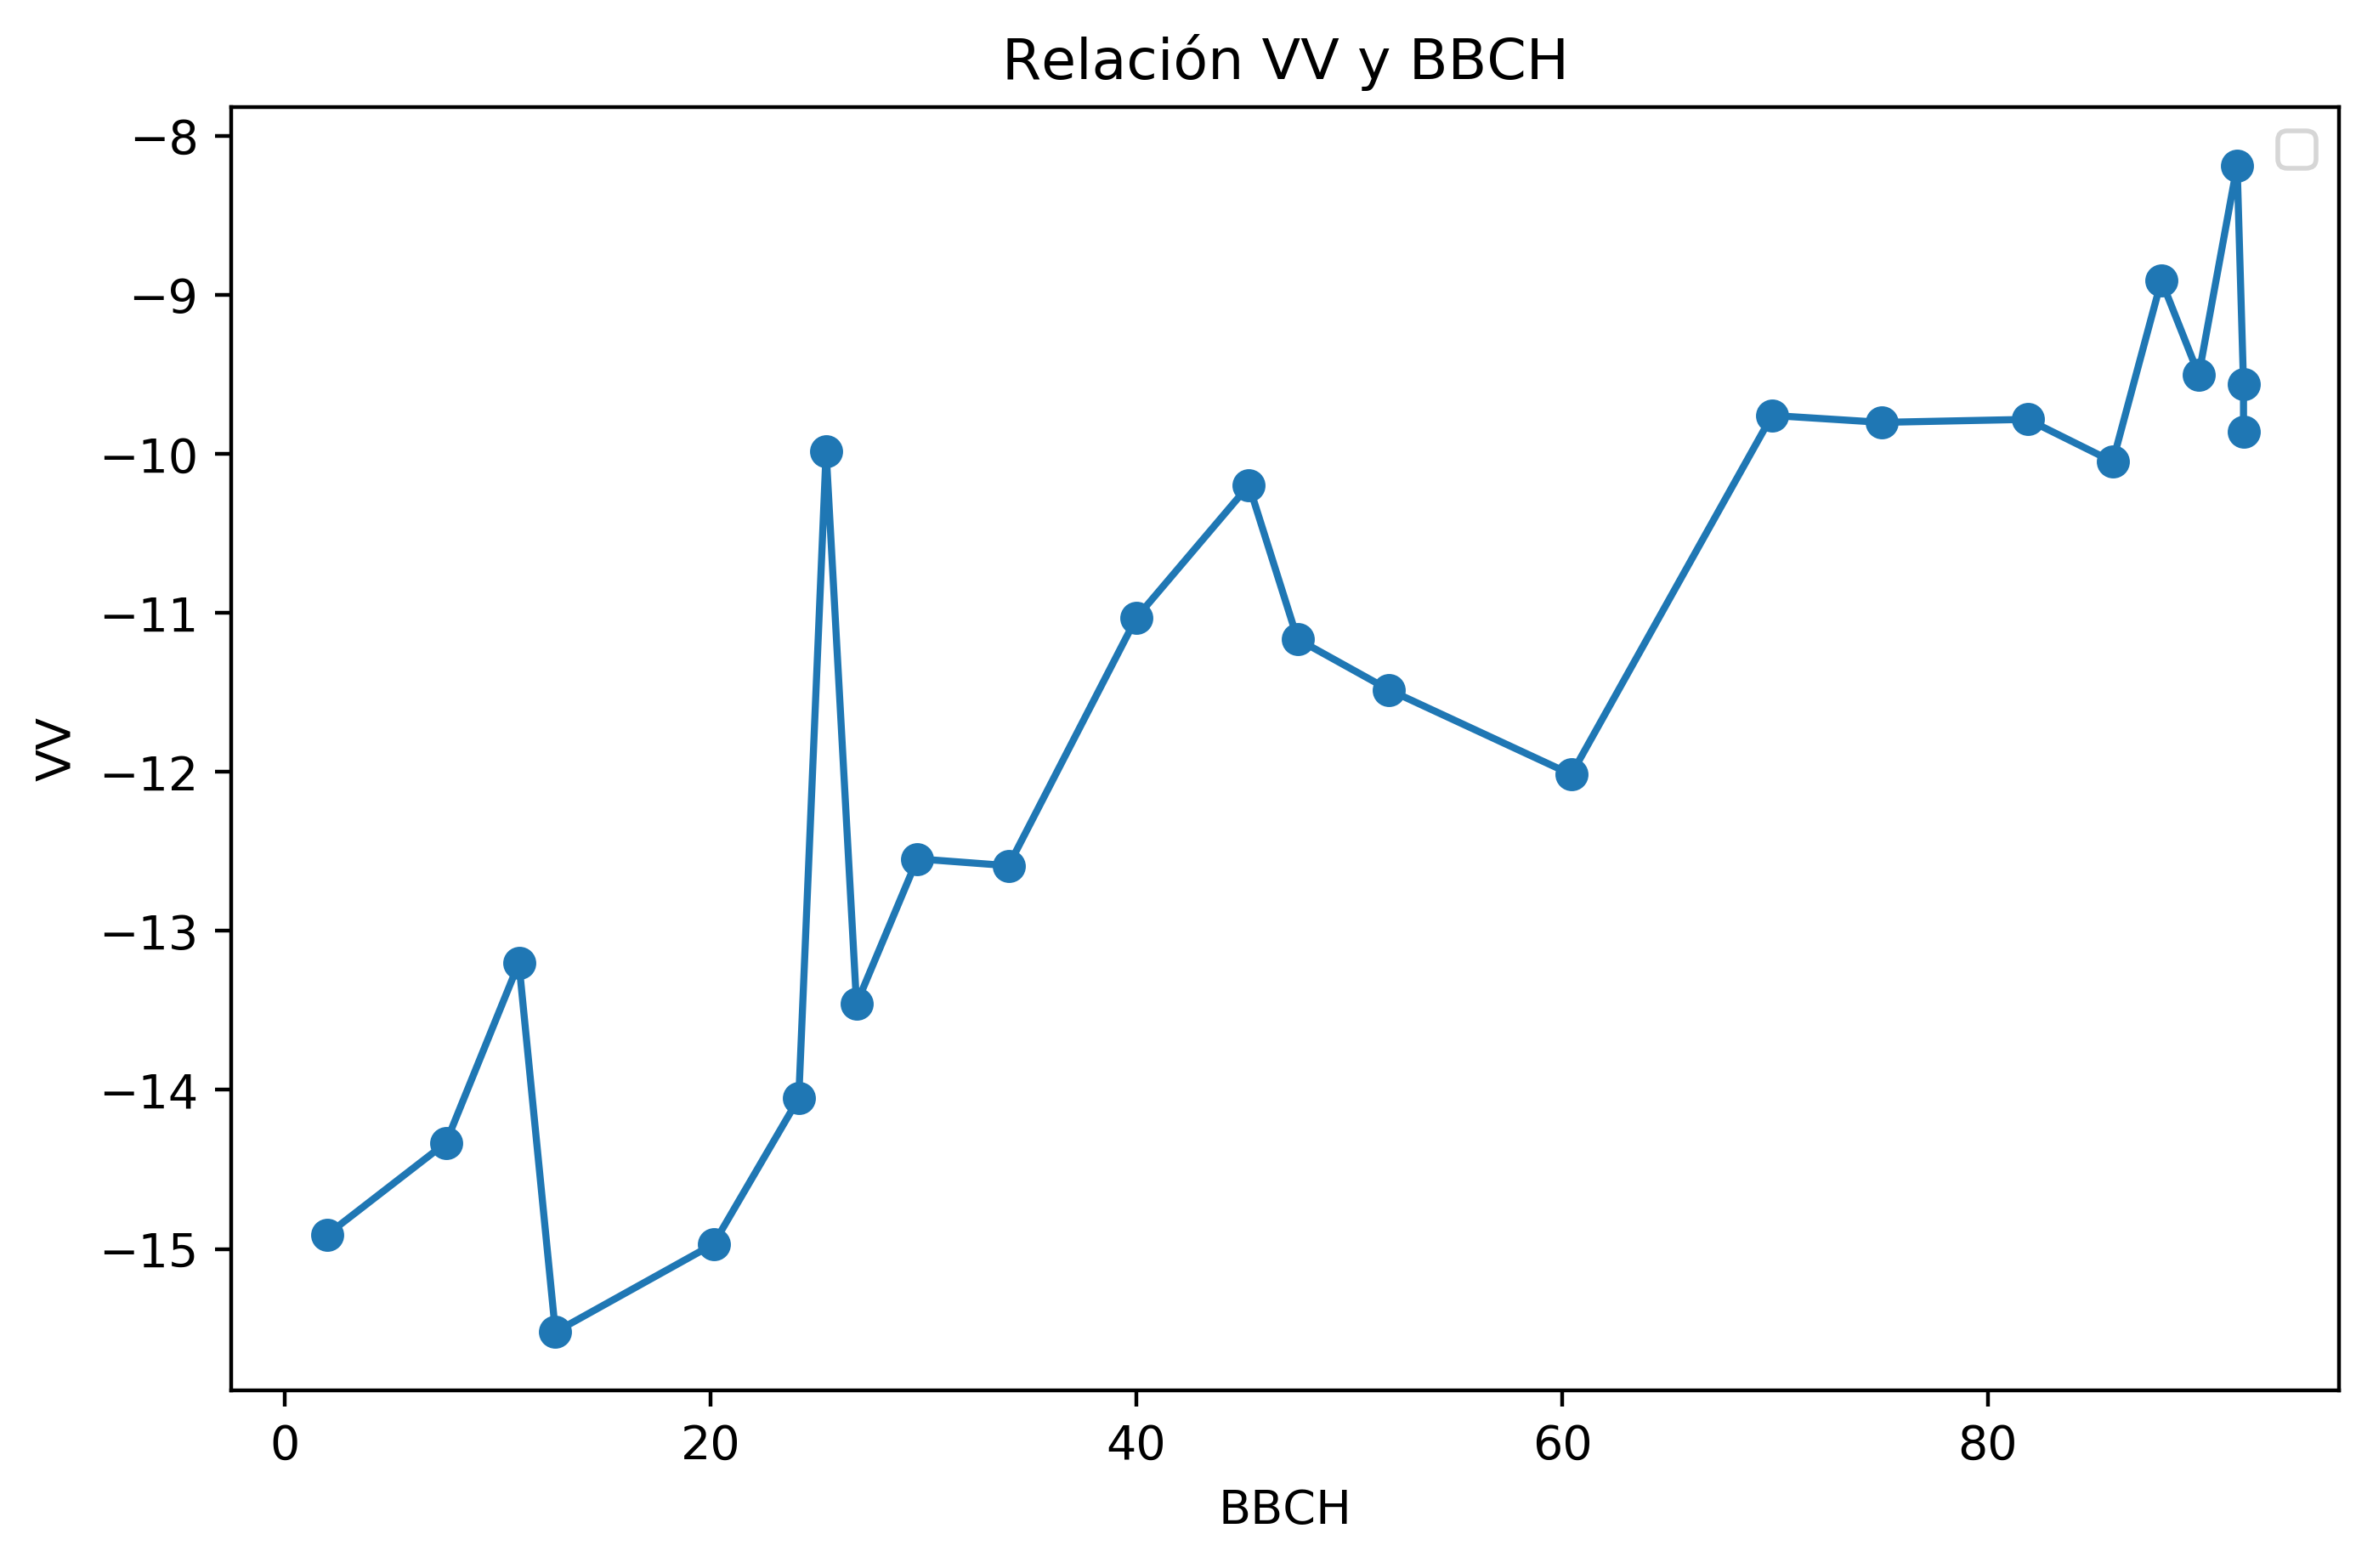
\includegraphics[width=\linewidth]{archivos/VV}
  \caption{Relación de la variable VV con respecto a la \gls{bbch}. \label{fig:VV}}
\end{subfigure}%
\begin{subfigure}{.45\textwidth}
  \centering
  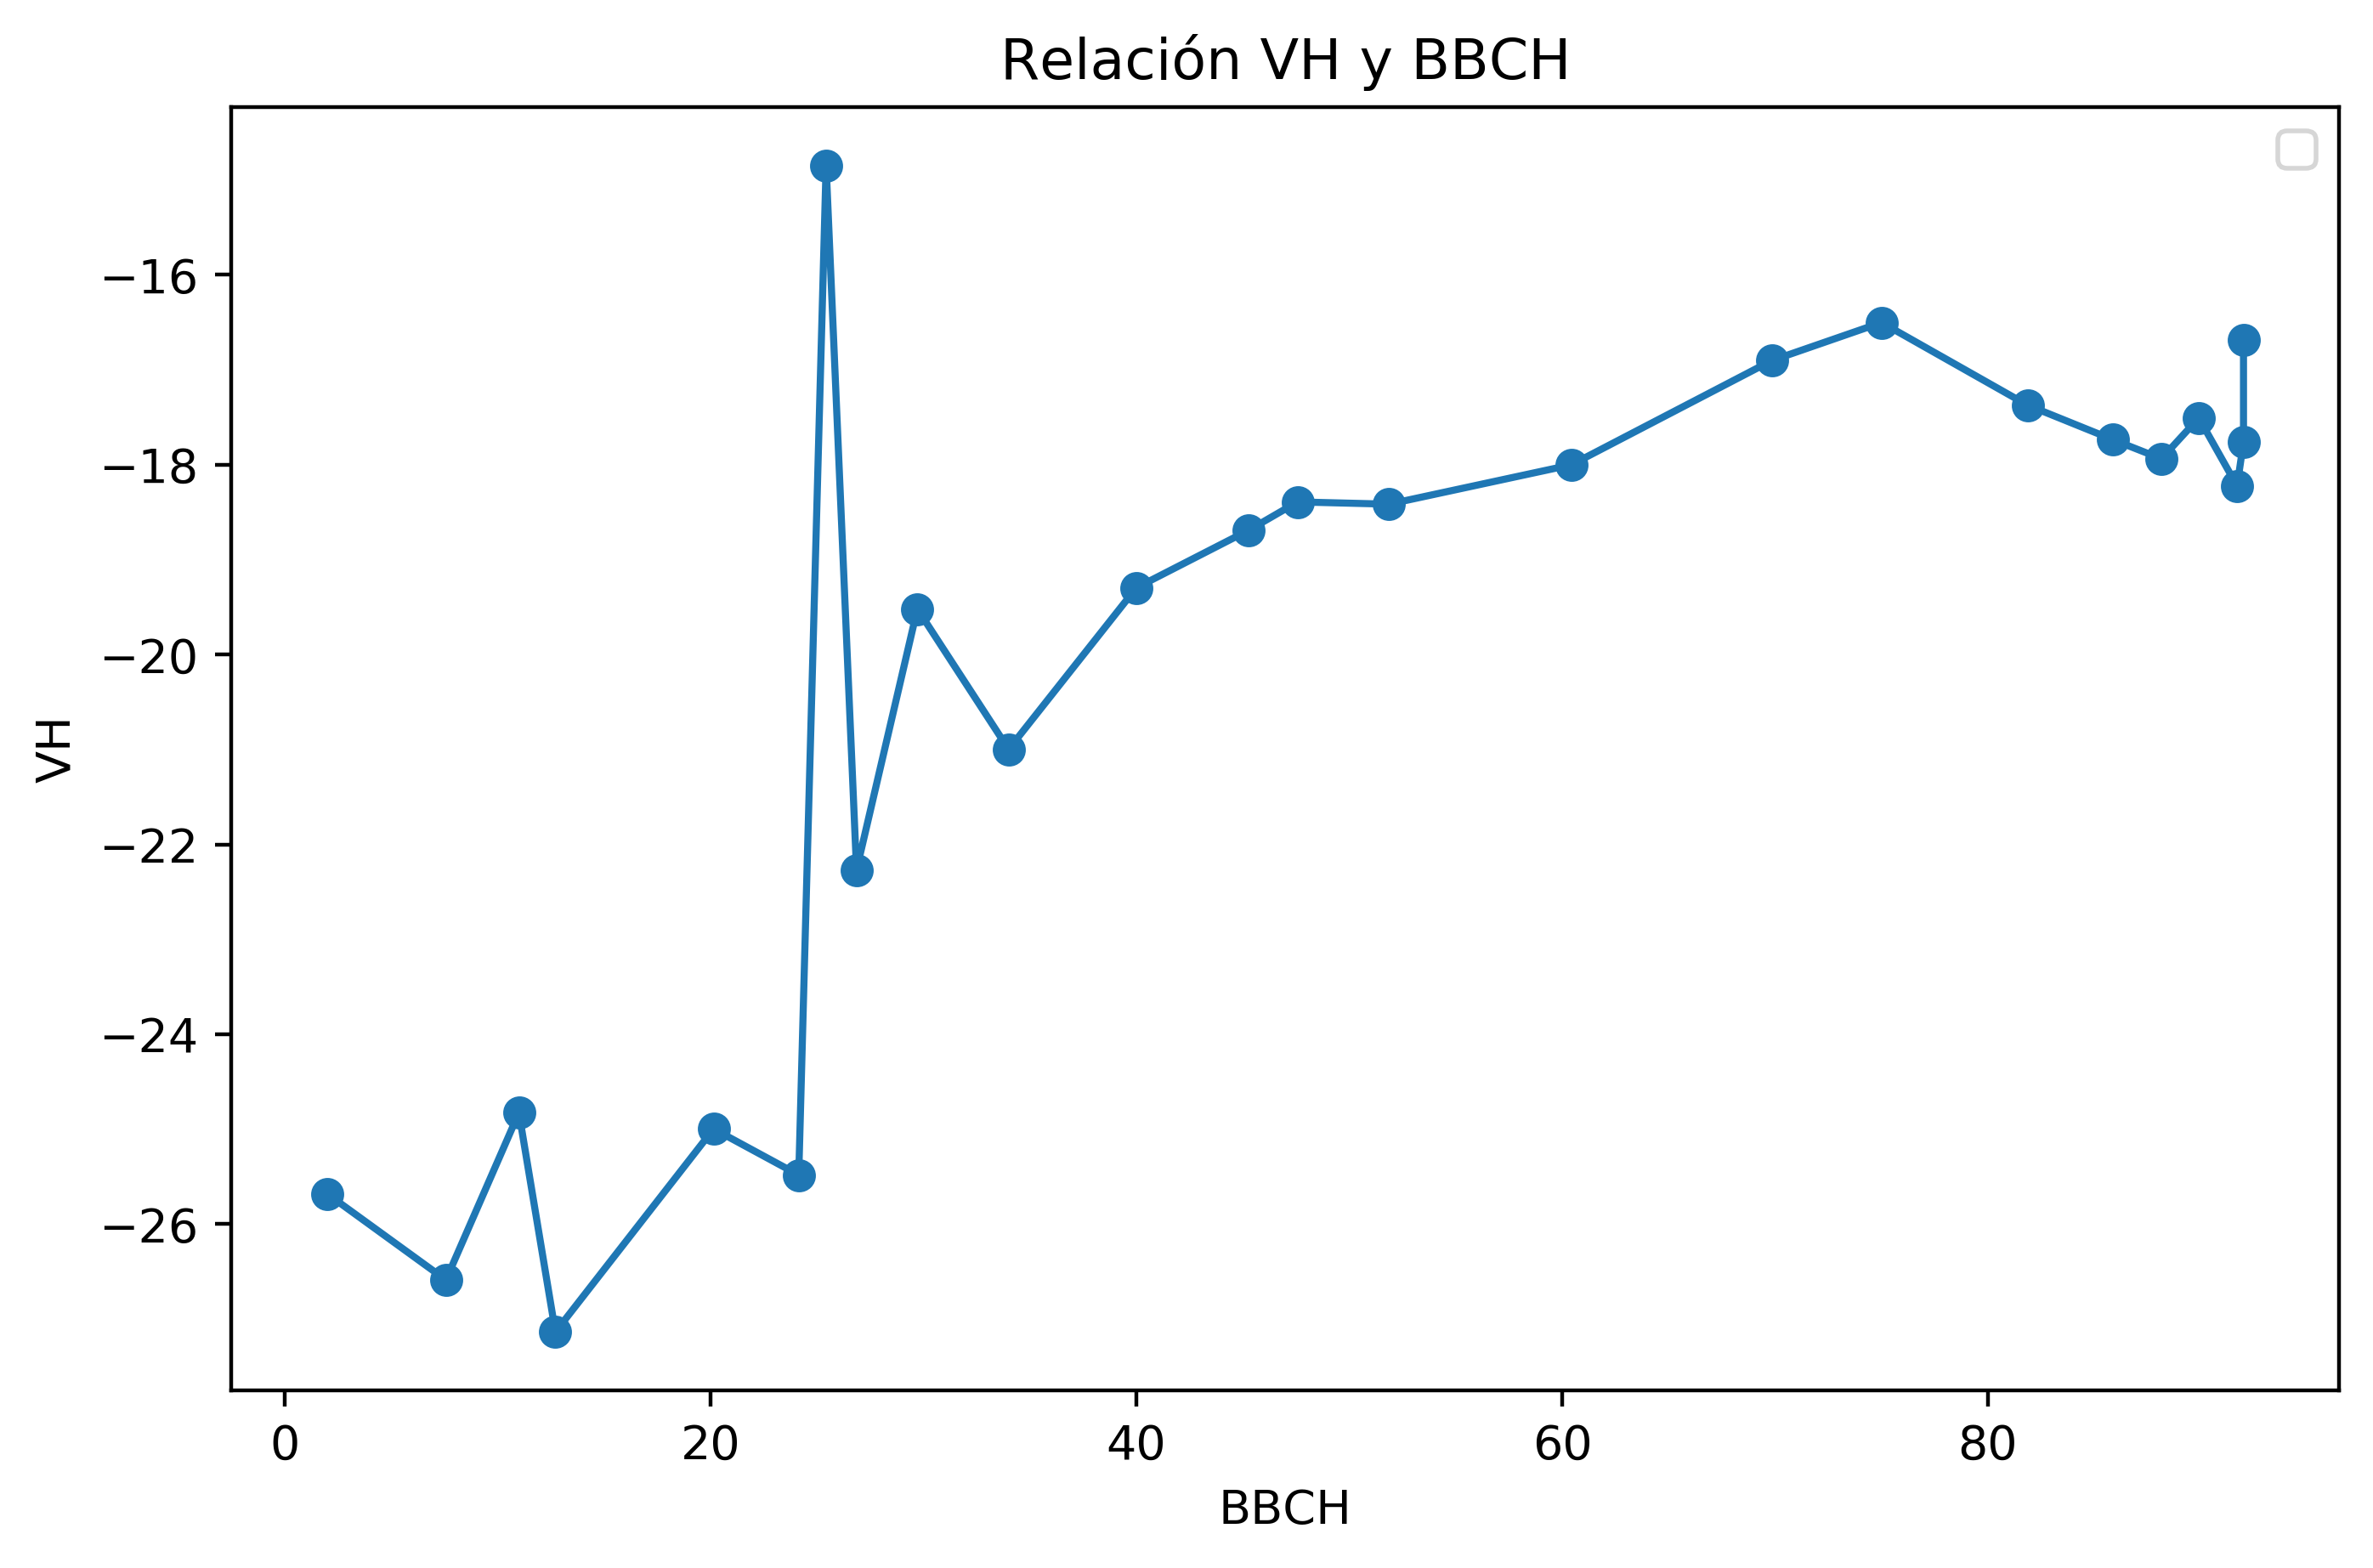
\includegraphics[width=\linewidth]{archivos/VH}
  \caption{Relación de la variable VH con respecto a la \gls{bbch}.\label{fig:VH}}
\end{subfigure}
\begin{subfigure}{.45\textwidth}
  \centering
  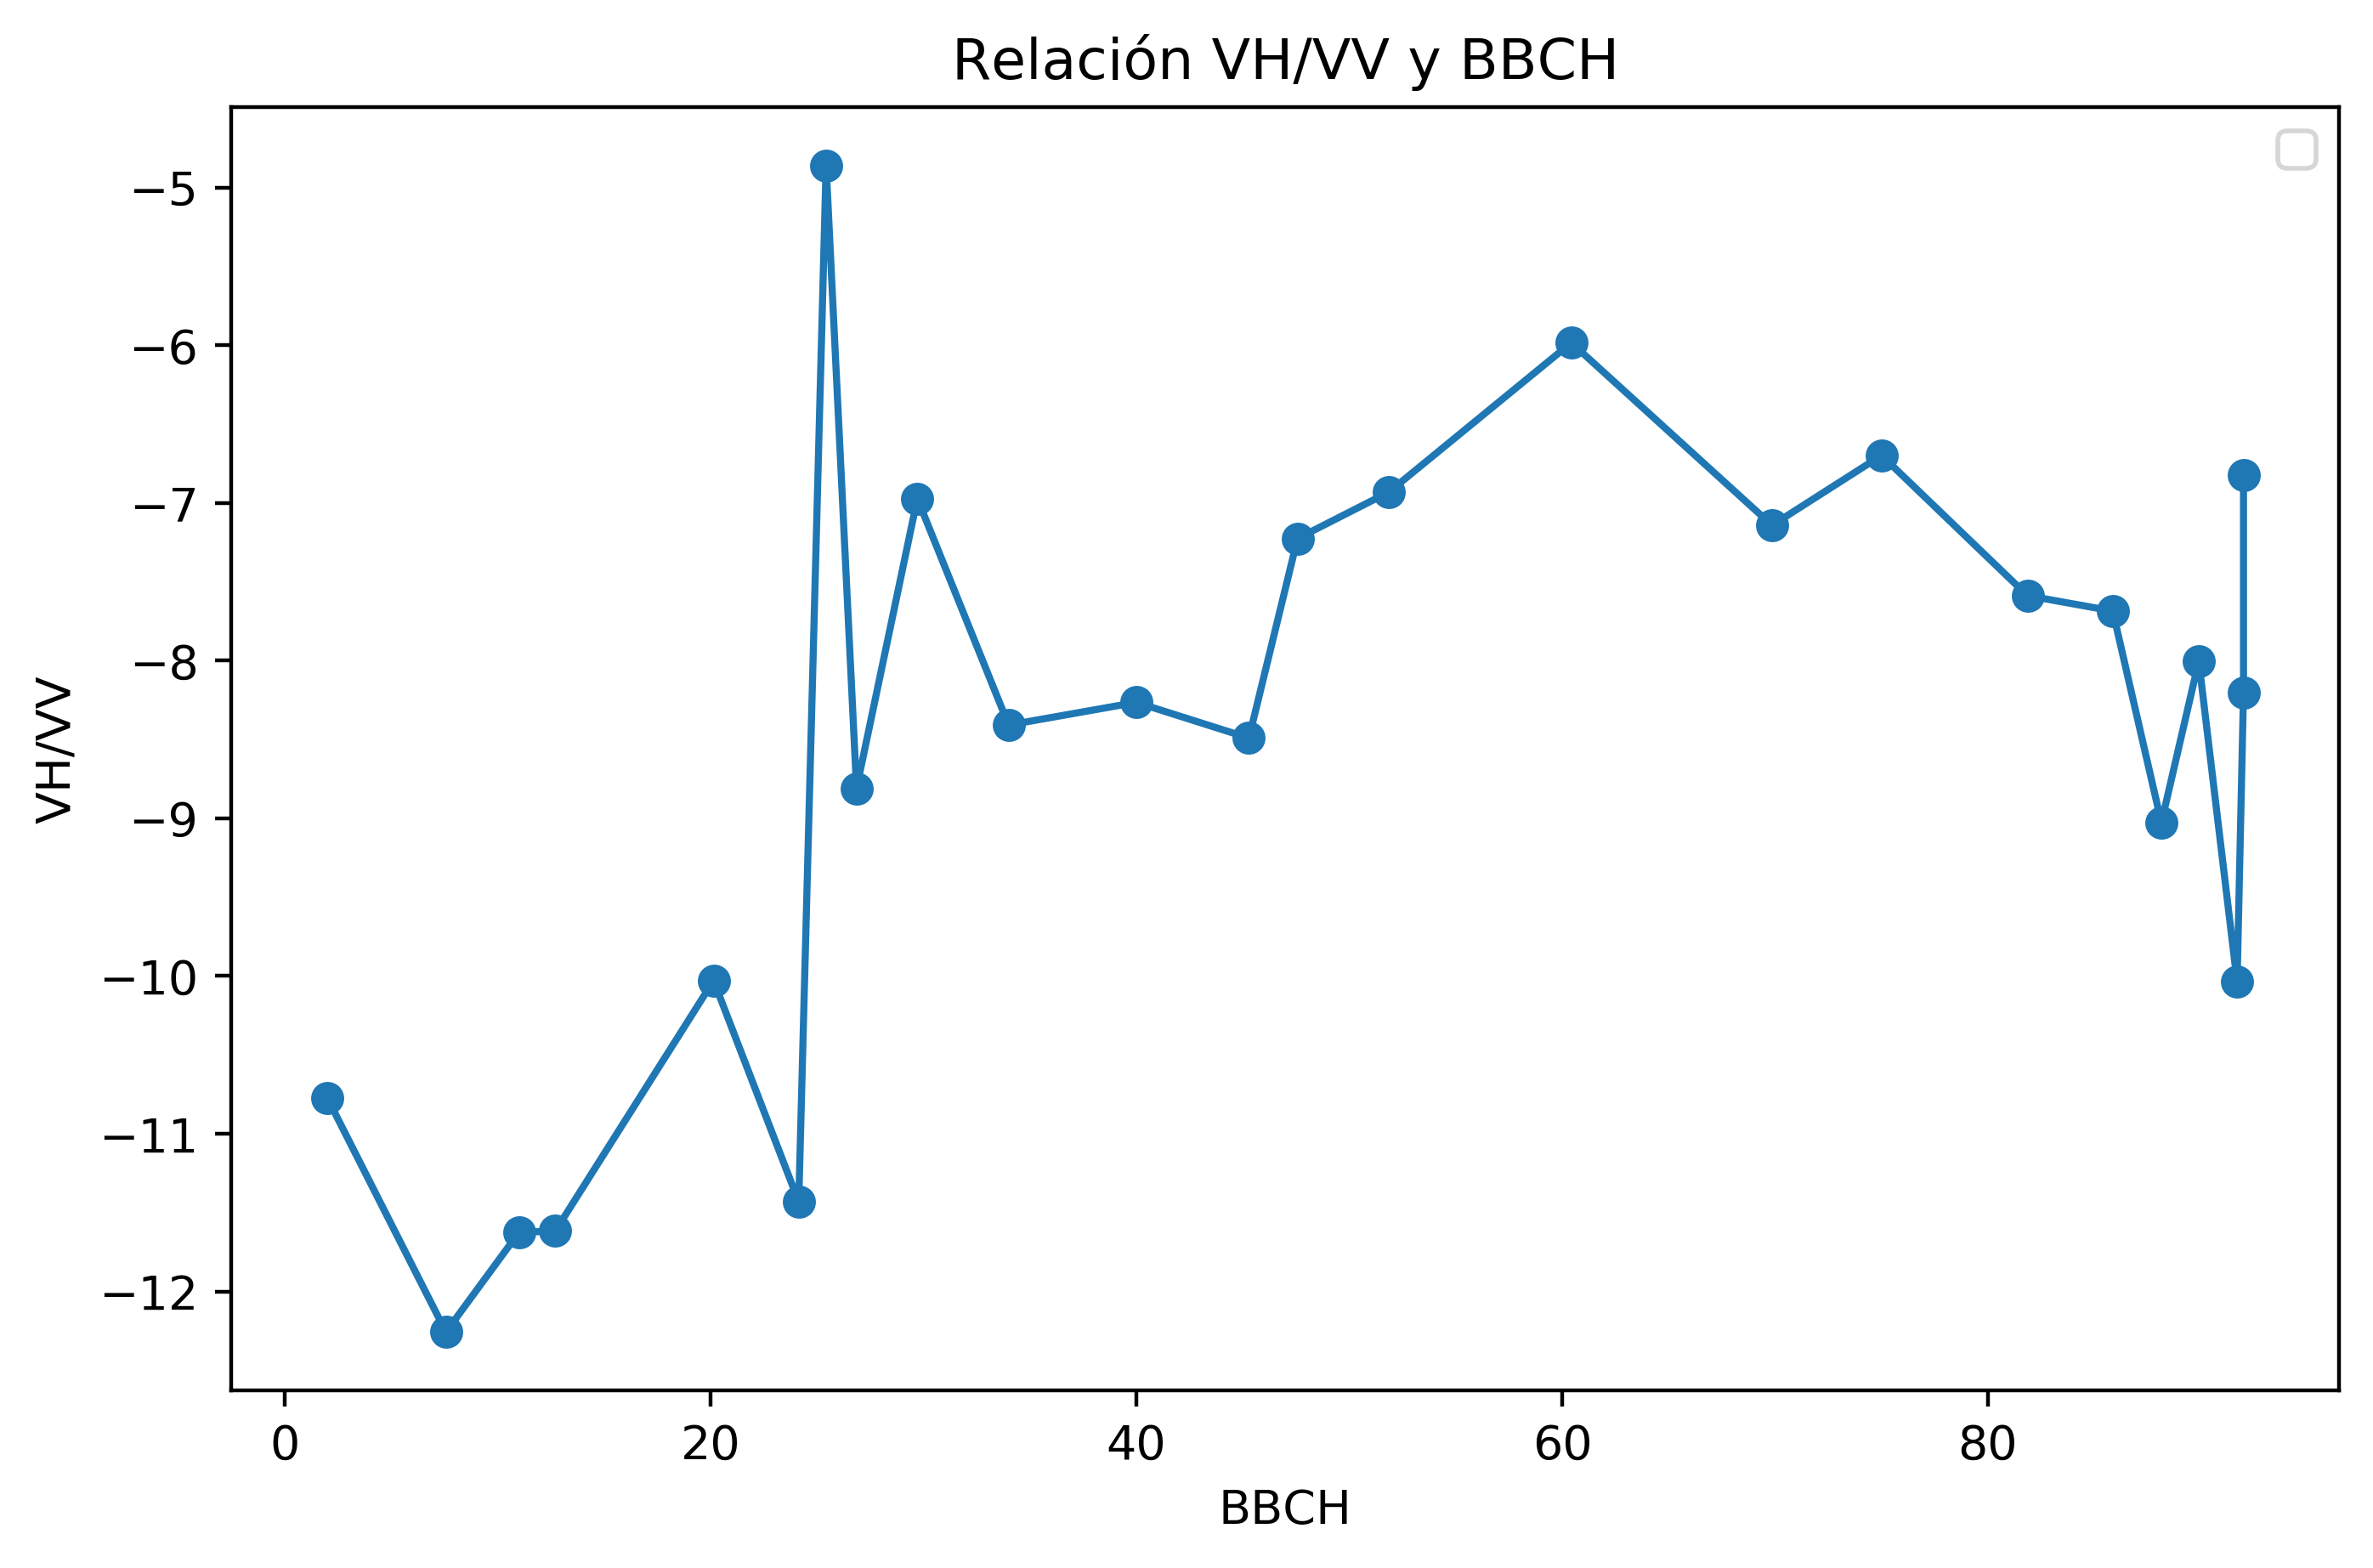
\includegraphics[width=\linewidth]{archivos/RATIO}
  \caption{Relación de la variable ratio VH/VV con respecto a la \gls{bbch}.\label{fig:RATIO}}
\end{subfigure}
\caption{Relación de las variables de datos de entrada al modelo con respecto a la \gls{bbch} \label{fig:rel_param}}
\end{figure}

%%%%%%%%%%%%%%%%%%%
%%%%%%%%%%%%%%%%%%%
\section{Método por píxeles} 
\subsection{Optimización}
\par La optimización de los datos de entrada para este método se realiza de igual manera que el anterior, coincidiendo los mejores resultados para todos los casos en el uso de un conjunto de 6 parcelas para entrenamiento y 1 para la evaluación y los datos de entrada, se reducen a los tres principales (VV, VH y ratio), ya que la desviación estándar no aporta una gran mejora para este método. En cuanto a la optimización del regresor, se utiliza también la relación entre el número de árboles para un modelo y el coeficiente de determinación, presentado en la imagen de ejemplo \ref{fig:opt_pixl} con el caso de salida \gls{bbch}. En ella, se puede ver que una vez alcanzado cierto nivel de coeficiente, la mejora de este en relación al aumento del número de árboles no es significativa con respecto al costo computacional y a la complejidad del sistema que se crea. 
\begin{figure}[h]
    \centering
    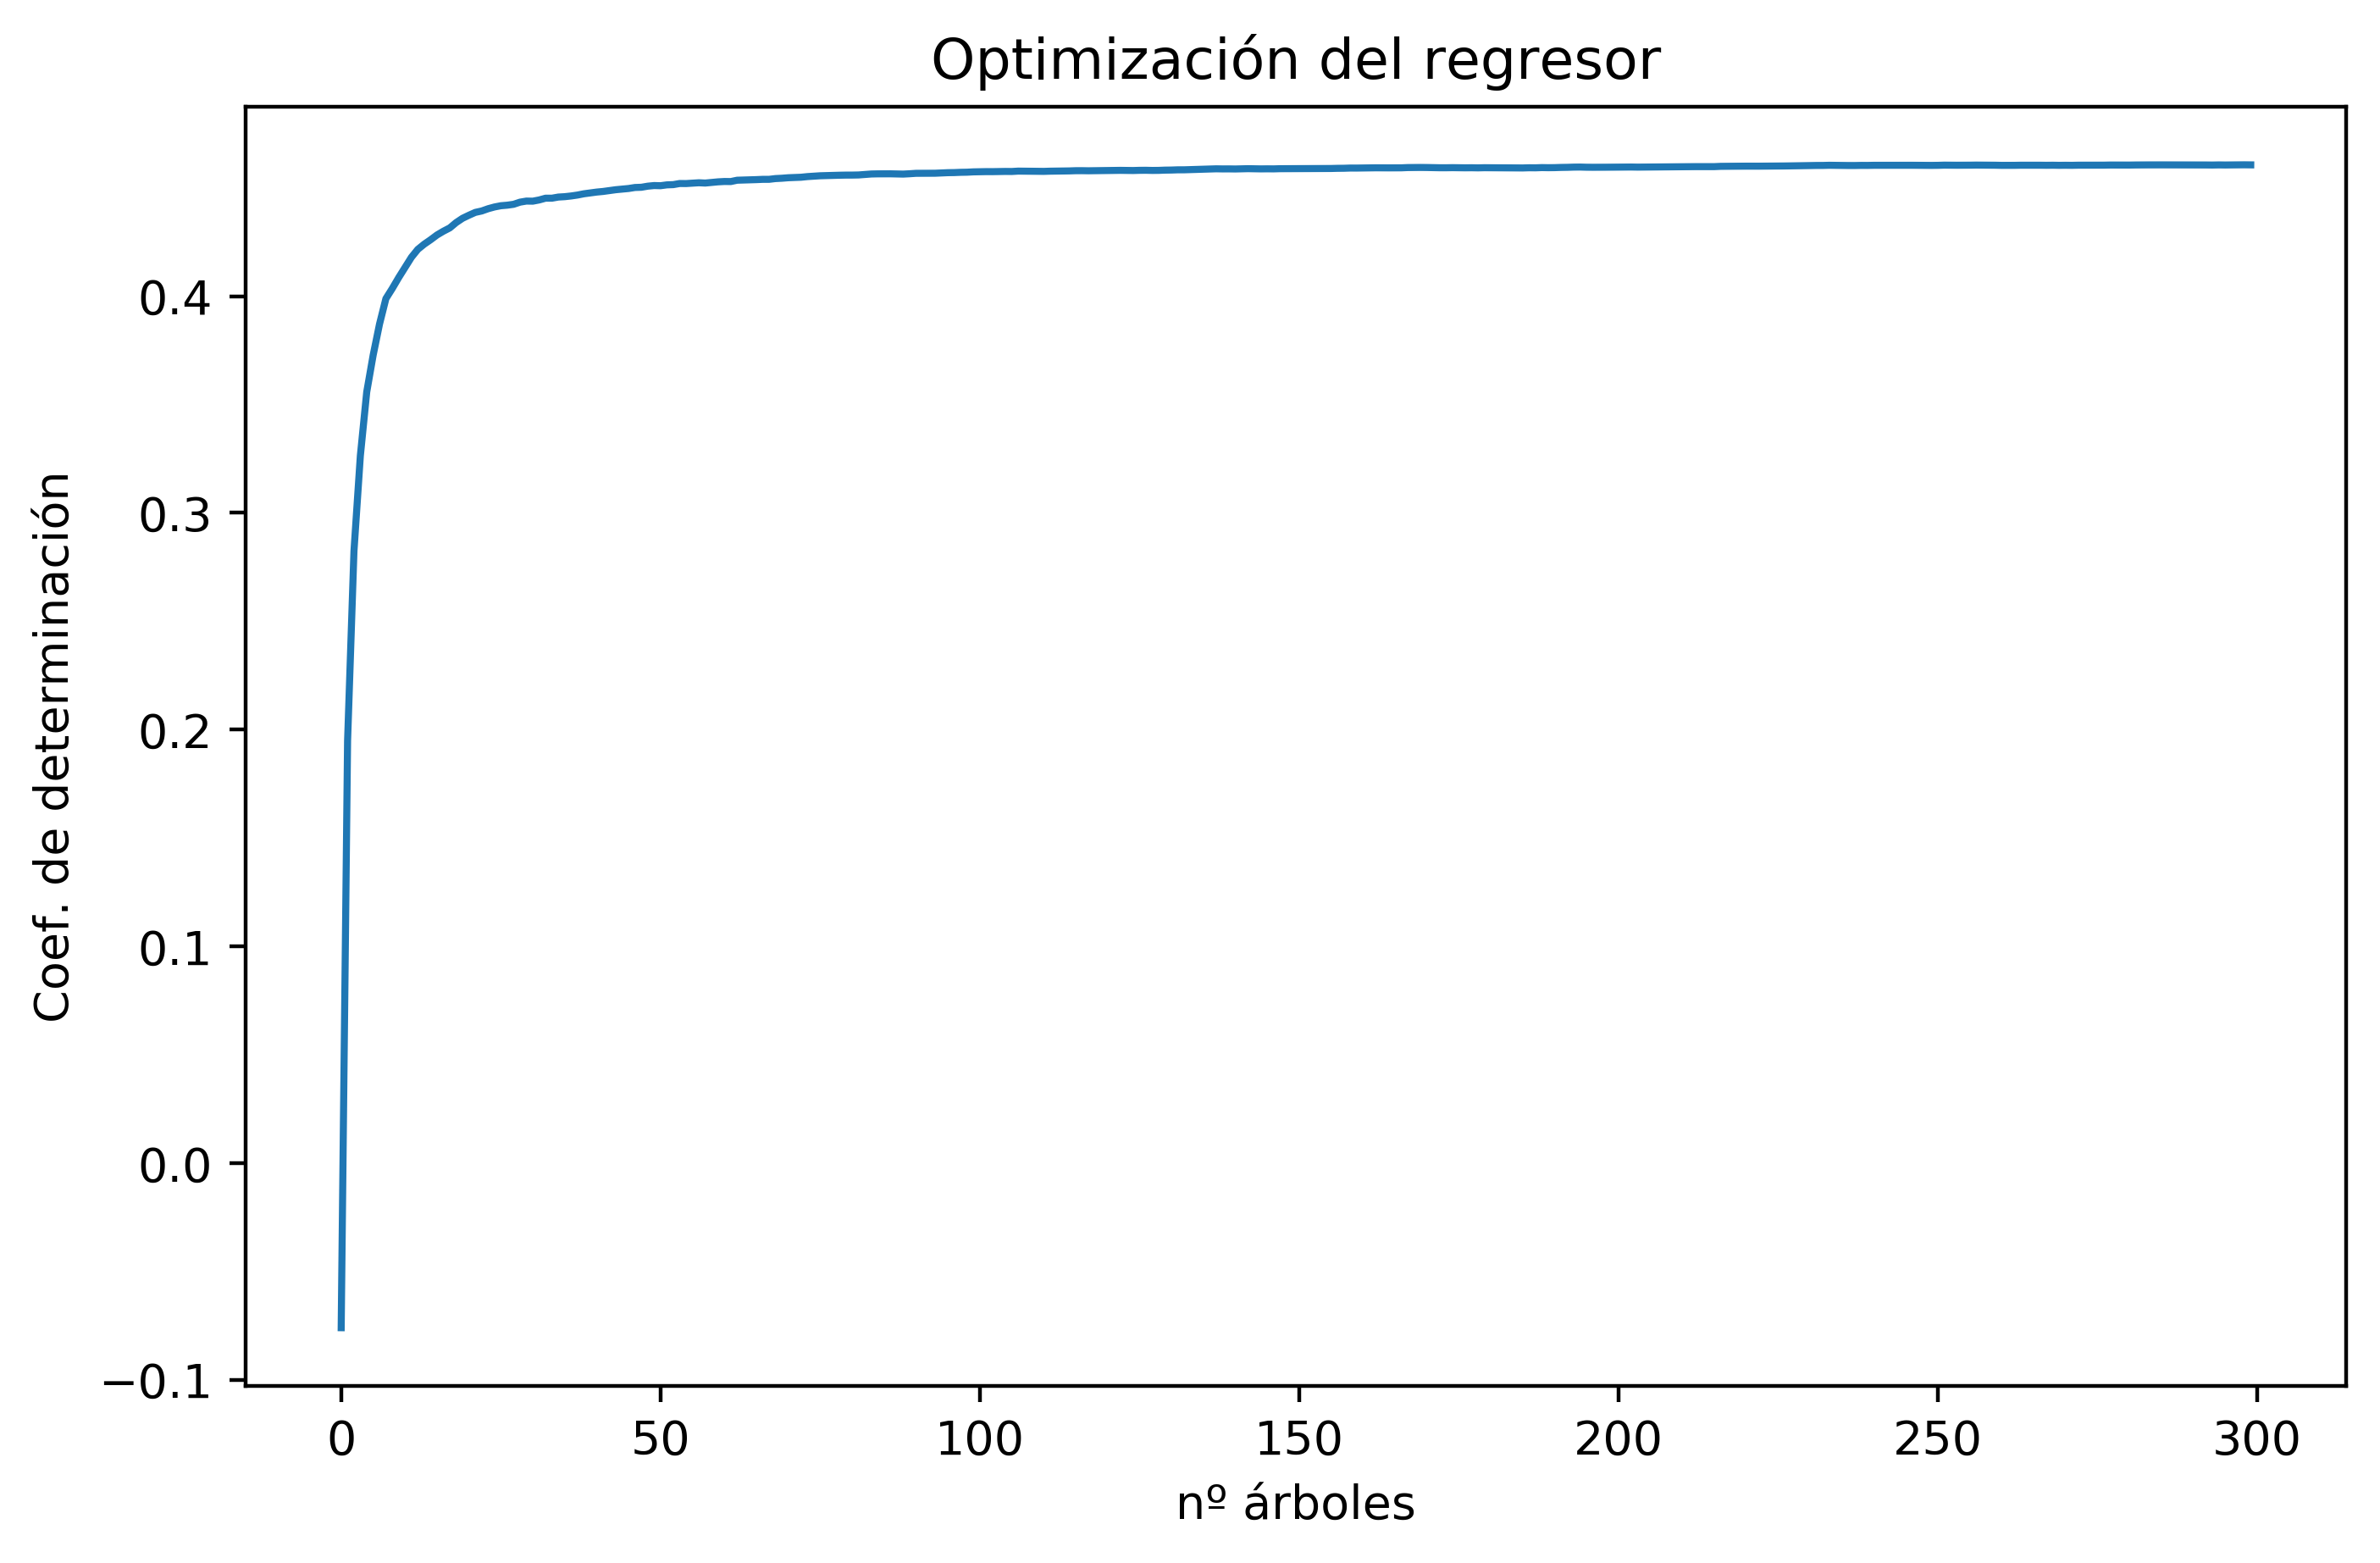
\includegraphics[height=9cm]{archivos/tfg/Pixel/opt_tree_bbch_pixel} 
    \caption{Optimización del número de árboles para \gls{rfr} en el modelo de salida \gls{bbch}}
    \label{fig:opt_pixl}
\end{figure}

\par Finalmente, los parámetros utilizados en este método para cada caso se presentan en la tabla \ref{tab:opt_pixl}, donde se pueden ver: la parcela utilizada para el periodo de test del modelo; siendo el resto de parcelas utilizadas en el entrenamiento, y el número de árboles óptimo para \gls{rfr}, de acuerdo con la evolución del coeficiente de determinación para cada caso.

\begin{table}[h]
\centering
\begin{tabular}{l|ccc}
                  & \gls{bbch}     & Altura   & \gls{bbch}\&Altura \\ \hline
Parcela de test   & `Mínima' & `Mínima' & `Mínima'     \\
Número de árboles & 46       & 48       & 47          
\end{tabular}
\caption{Parámetros de optimización de entrada y modelo \label{tab:opt_pixl}}
\end{table}

\par Como se puede observar, los 3 casos coinciden en el set de parcelas de entrenamiento y test con el que se obtienen mejores resultados. Probablemente esto se debe a anomalías en el desarrollo de algunas parcelas, las cuales, si se toman como set de test, el modelo no las habría podido tener en cuenta en el aprendizaje y el error en la predicción sería mayor. Los 3 casos de este método constan de un número óptimo de árboles muy similares, con una diferencia de 1 y 2 con respecto al caso menor. Cabe destacar que el aumento de complejidad, aunque escaso, en el modelo de salida de la altura, como ocurre para el método anterior. Además, tanto para la metodología por píxeles como por parcelas, se obtiene un número óptimo de árboles para el caso de 2 salidas intermedio a los óptimos para las mismas salidas en modelos independientes. Esto se debe a una compensación en la estimación de ambas variables, para que una variable sea óptima sin que su mejora sea a costa de la otra se llega a un valor intermedio en el que ninguna de las salidas está totalmente optimizada pero tienen el mejor resultado del sistema compartido completo. 


\subsection{Salidas del modelo}
\subsubsection{Salidas de función de densidad de probabilidad}
Como se ha mencionado en la metodología anterior, las salidas útiles de este trabajo son las \gls{pdf}. En las figuras \ref{fig:p_pdf_b} (modelo de salida \gls{bbch}), \ref{fig:p_pdf_h} (modelo de salida altura) y \ref{fig:p_pdf_bh} (modelo de ambas salidas) se puede apreciar cómo son algunas de estas salidas en esta metodología, siendo ejemplos extraídos a partir de los mismos datos para los 3 casos estudiados. 
\\
% Dos figuras sueltas debajo de otra
\begin{figure}[h]
\centering
\begin{subfigure}{0.6\textwidth}
	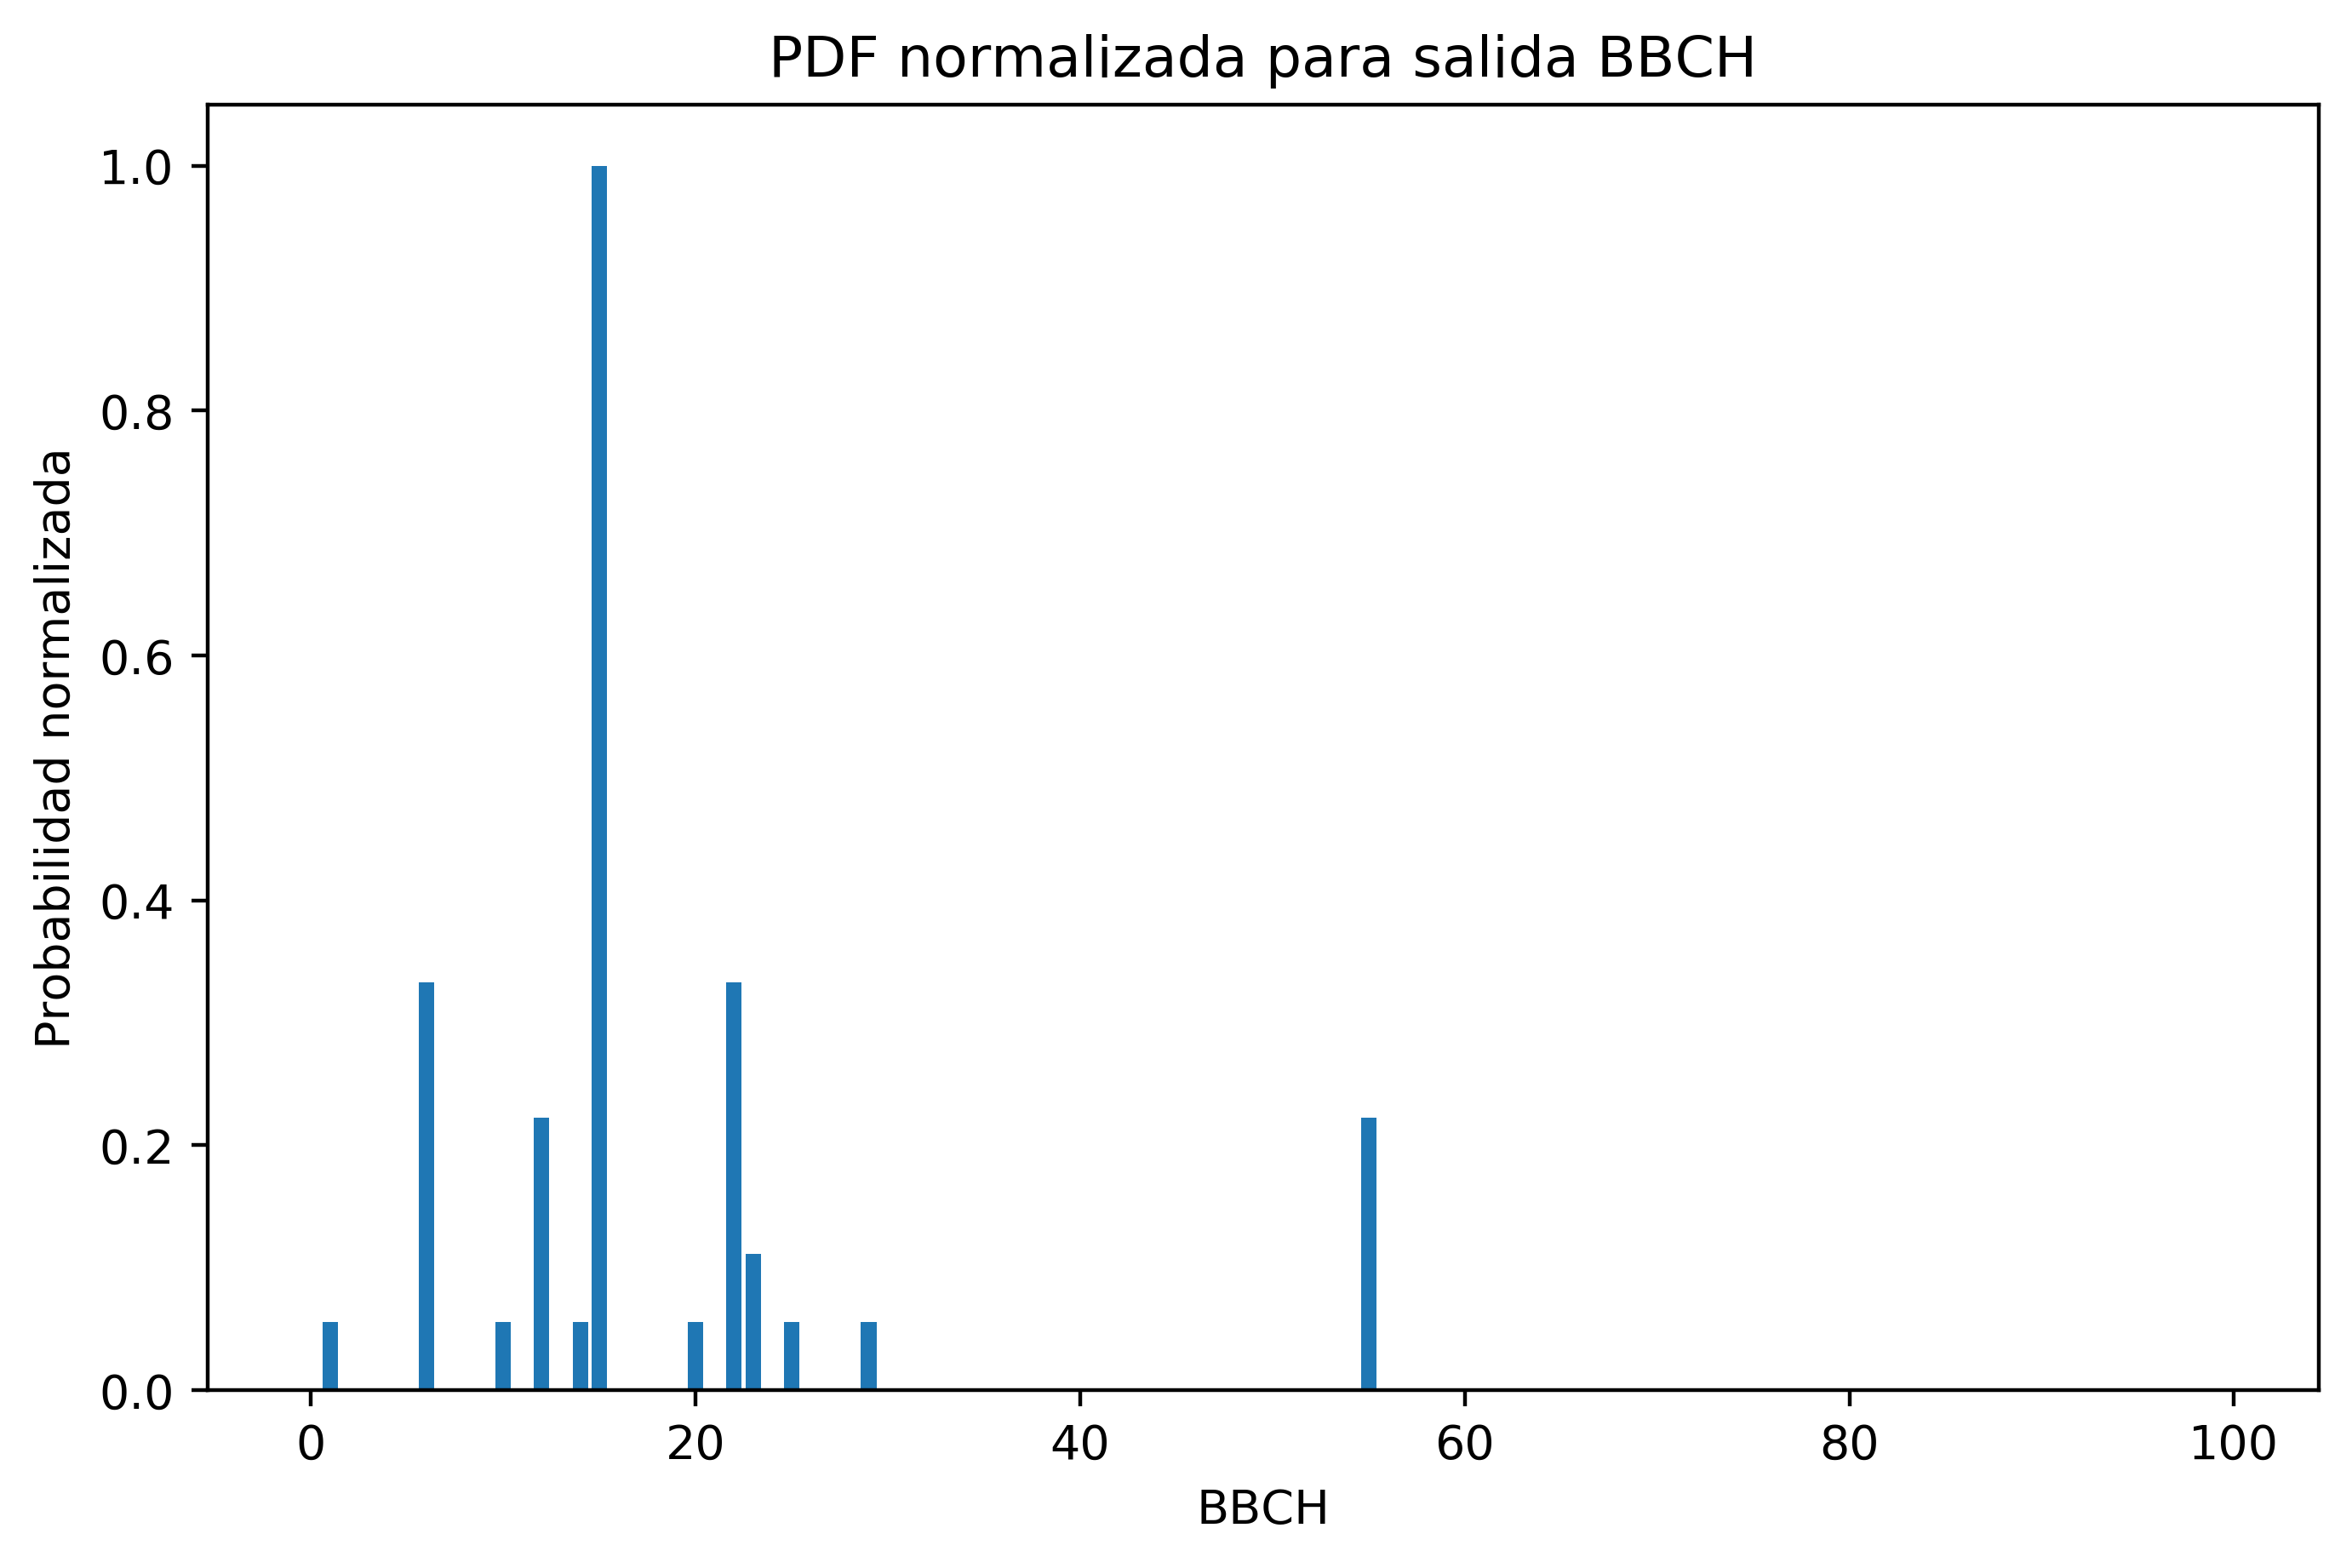
\includegraphics[width=\linewidth]{archivos/tfg/Pixel/BBCH_PDF}
	\caption{Ejemplo de salida \gls{pdf} normalizada del 			modelo para estimación de \gls{bbch}.\label{fig:p_pdf_b}}
\end{subfigure}
\begin{subfigure}{0.6\textwidth}
	\centering
	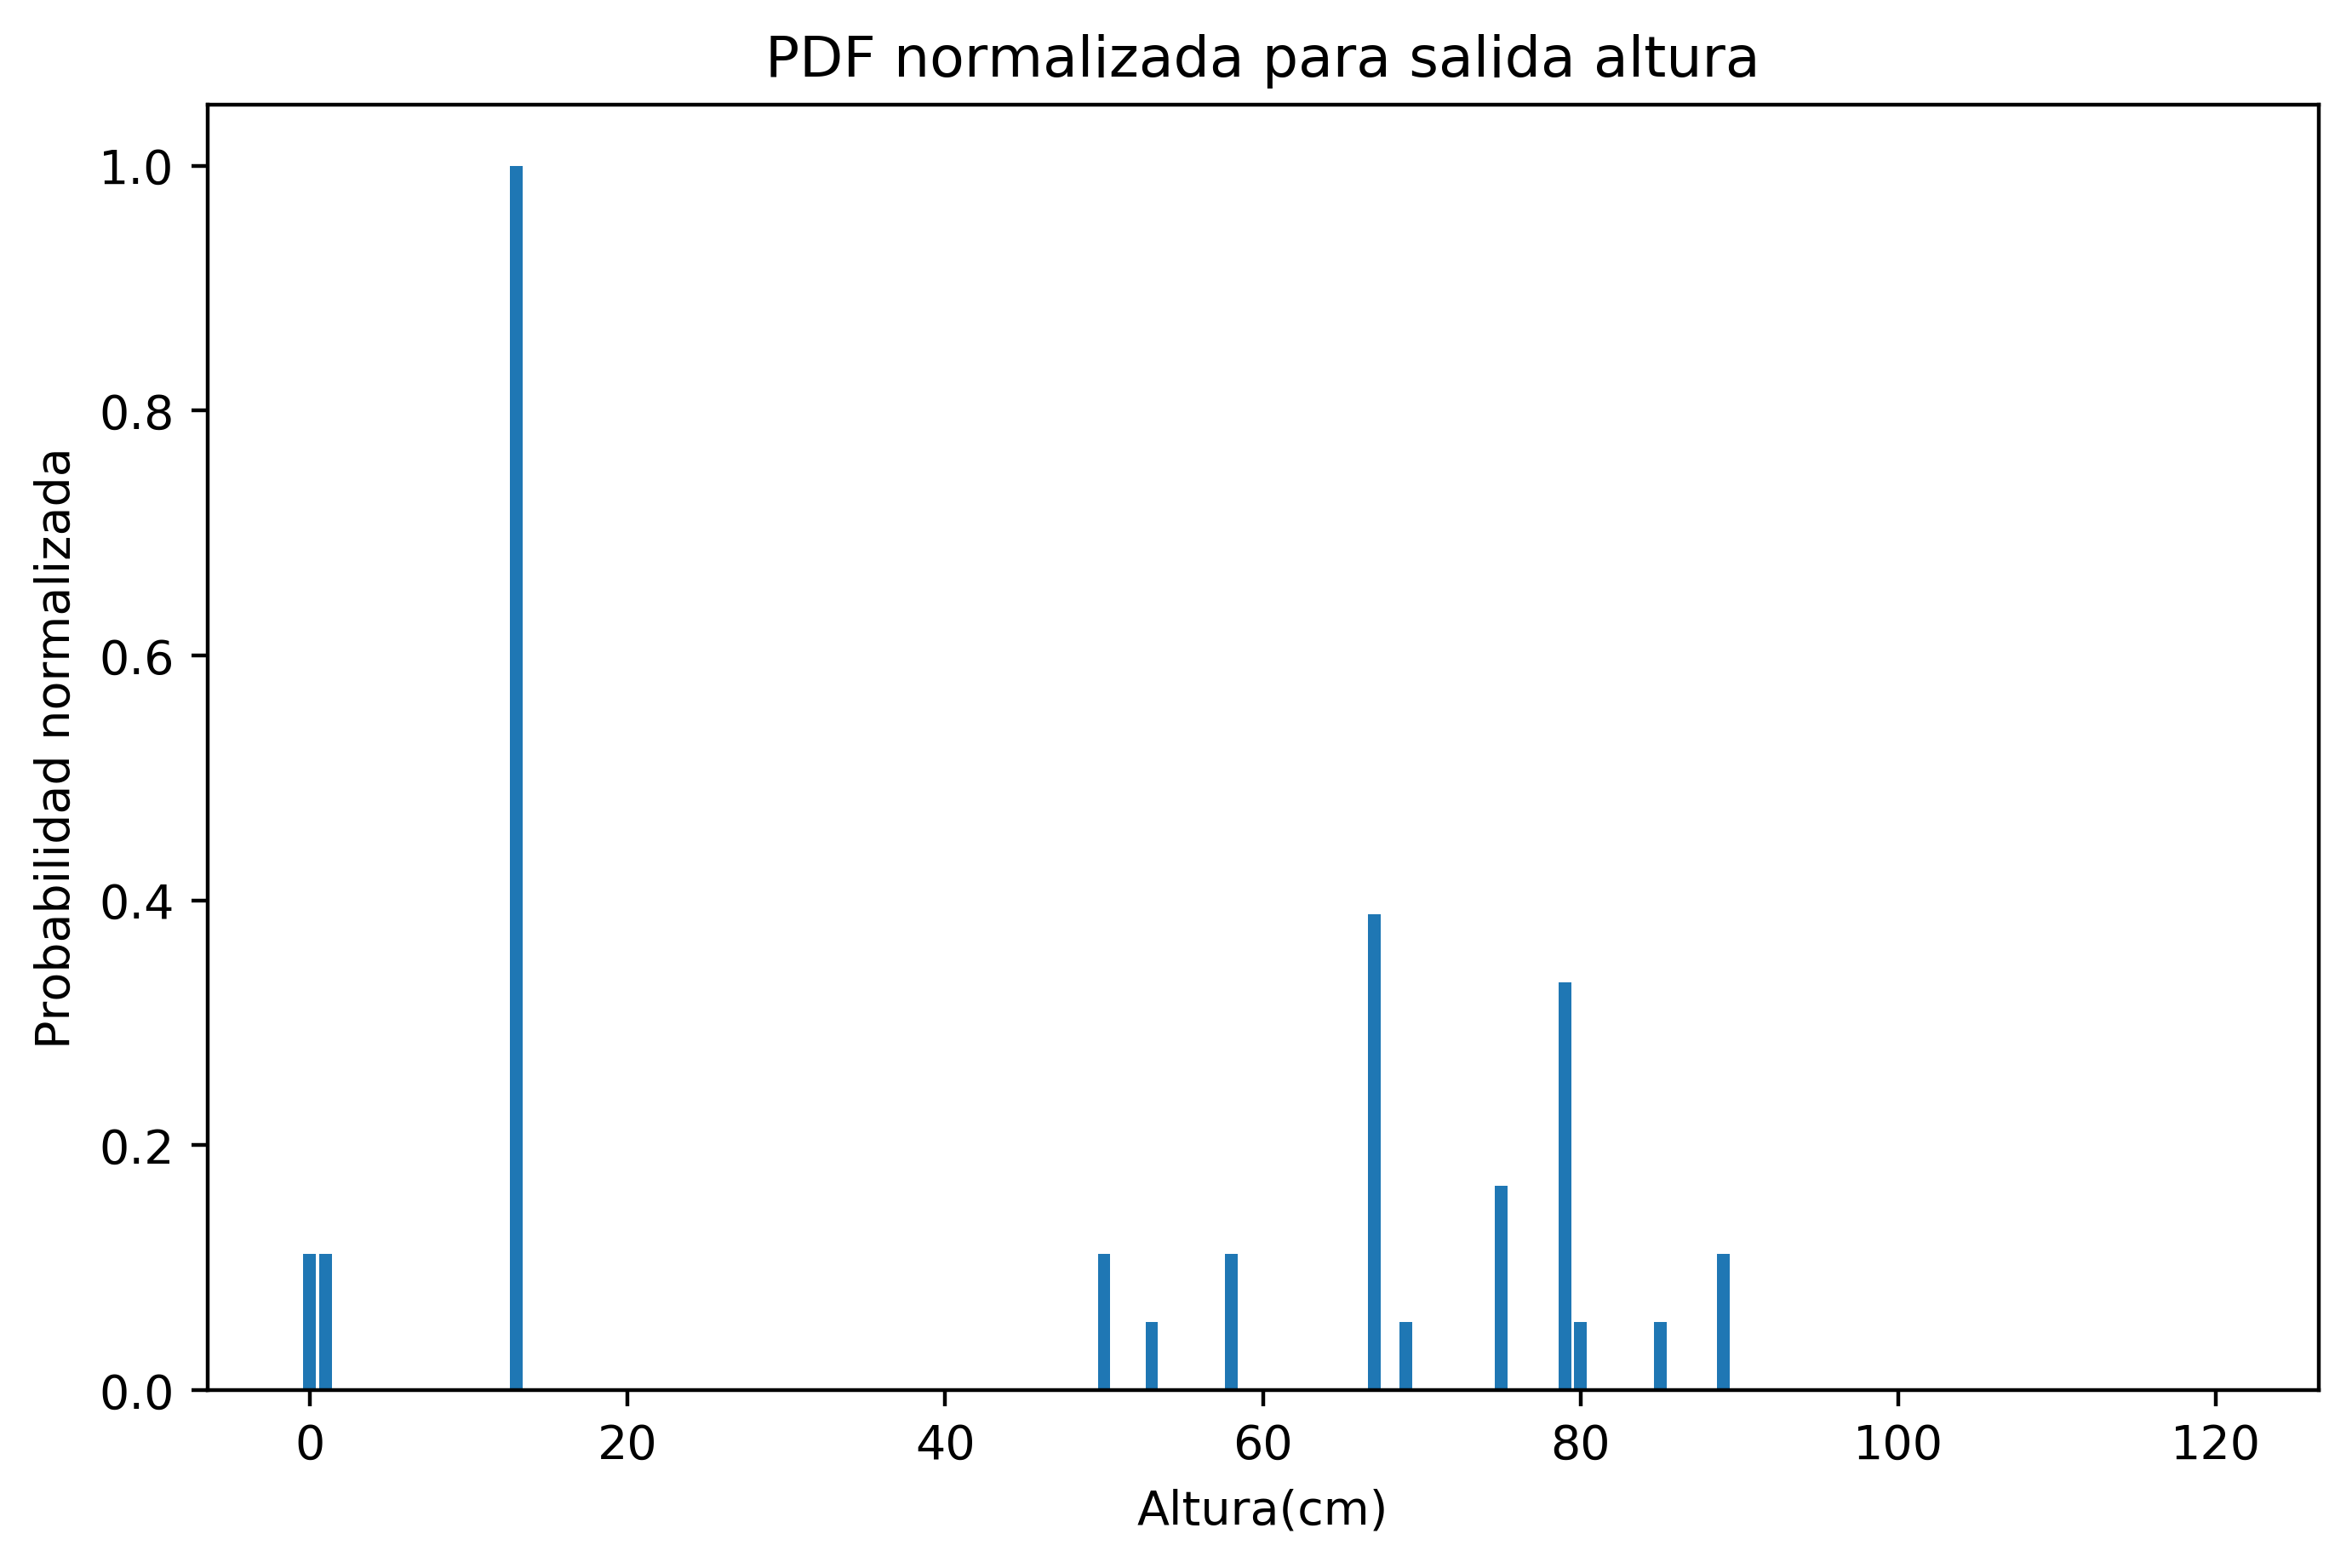
\includegraphics[width=\linewidth]{archivos/tfg/Pixel/H_PDF}
	\caption{Ejemplo de salida \gls{pdf} normalizada del 			modelo para estimación de la altura. \label{fig:p_pdf_h}}
	\end{subfigure}
	\caption{Ejemplo de salida \gls{pdf} normalizada los 			modelos para estimación de las variables independientes. \label{fig:p_pdf}}
\end{figure}

\par Estas representaciones tienen las mismas características mencionadas anteriormente: están normalizadas con respecto a la salida con mayor probabilidad, destaca una salida predominante pero no se excluyen el resto a la hora de integrarse con el modelo de predicción temporal. 
\\
\par Las figuras \ref{fig:p_pdf} y \ref{fig:p_pdf_bh} han sido generadas con los mismos datos de entrada, es decir, los mismos datos de satélite en la misma parcela y fecha, por lo que las salidas para los modelos generados de estimación de \gls{bbch} (Figura \ref{fig:p_pdf_b}) y altura (Figura \ref{fig:p_pdf_h}) como modelos independientes se pueden comparar con las salidas del modelo de estimación de ambas (Figura \ref{fig:p_pdf_bh}). La principal diferencia que se vuelve a encontrar entre los mismos tipos de datos de salida para cada modelo es que, las salidas individuales presentan una estimación principal con una diferencia de probabilidad mayor con respecto al resto que las estimaciones del modelo de doble salida. El rango para cada salida es bastante más amplio y disperso para el modelo de doble salida, esto junto a la disminución de diferencias con las demás estimaciones, indica que ese sistema es menos preciso y estable. En este modelo de dos salidas no se ve una clara optimización para una de ellas con respecto a la otra,  ya que además ambas tiene valores muy cercanos al sistema individual.

% Una figura con dos imágenes
\begin{figure}[H]
\centering
\begin{subfigure}{0.6\textwidth}
  \centering
  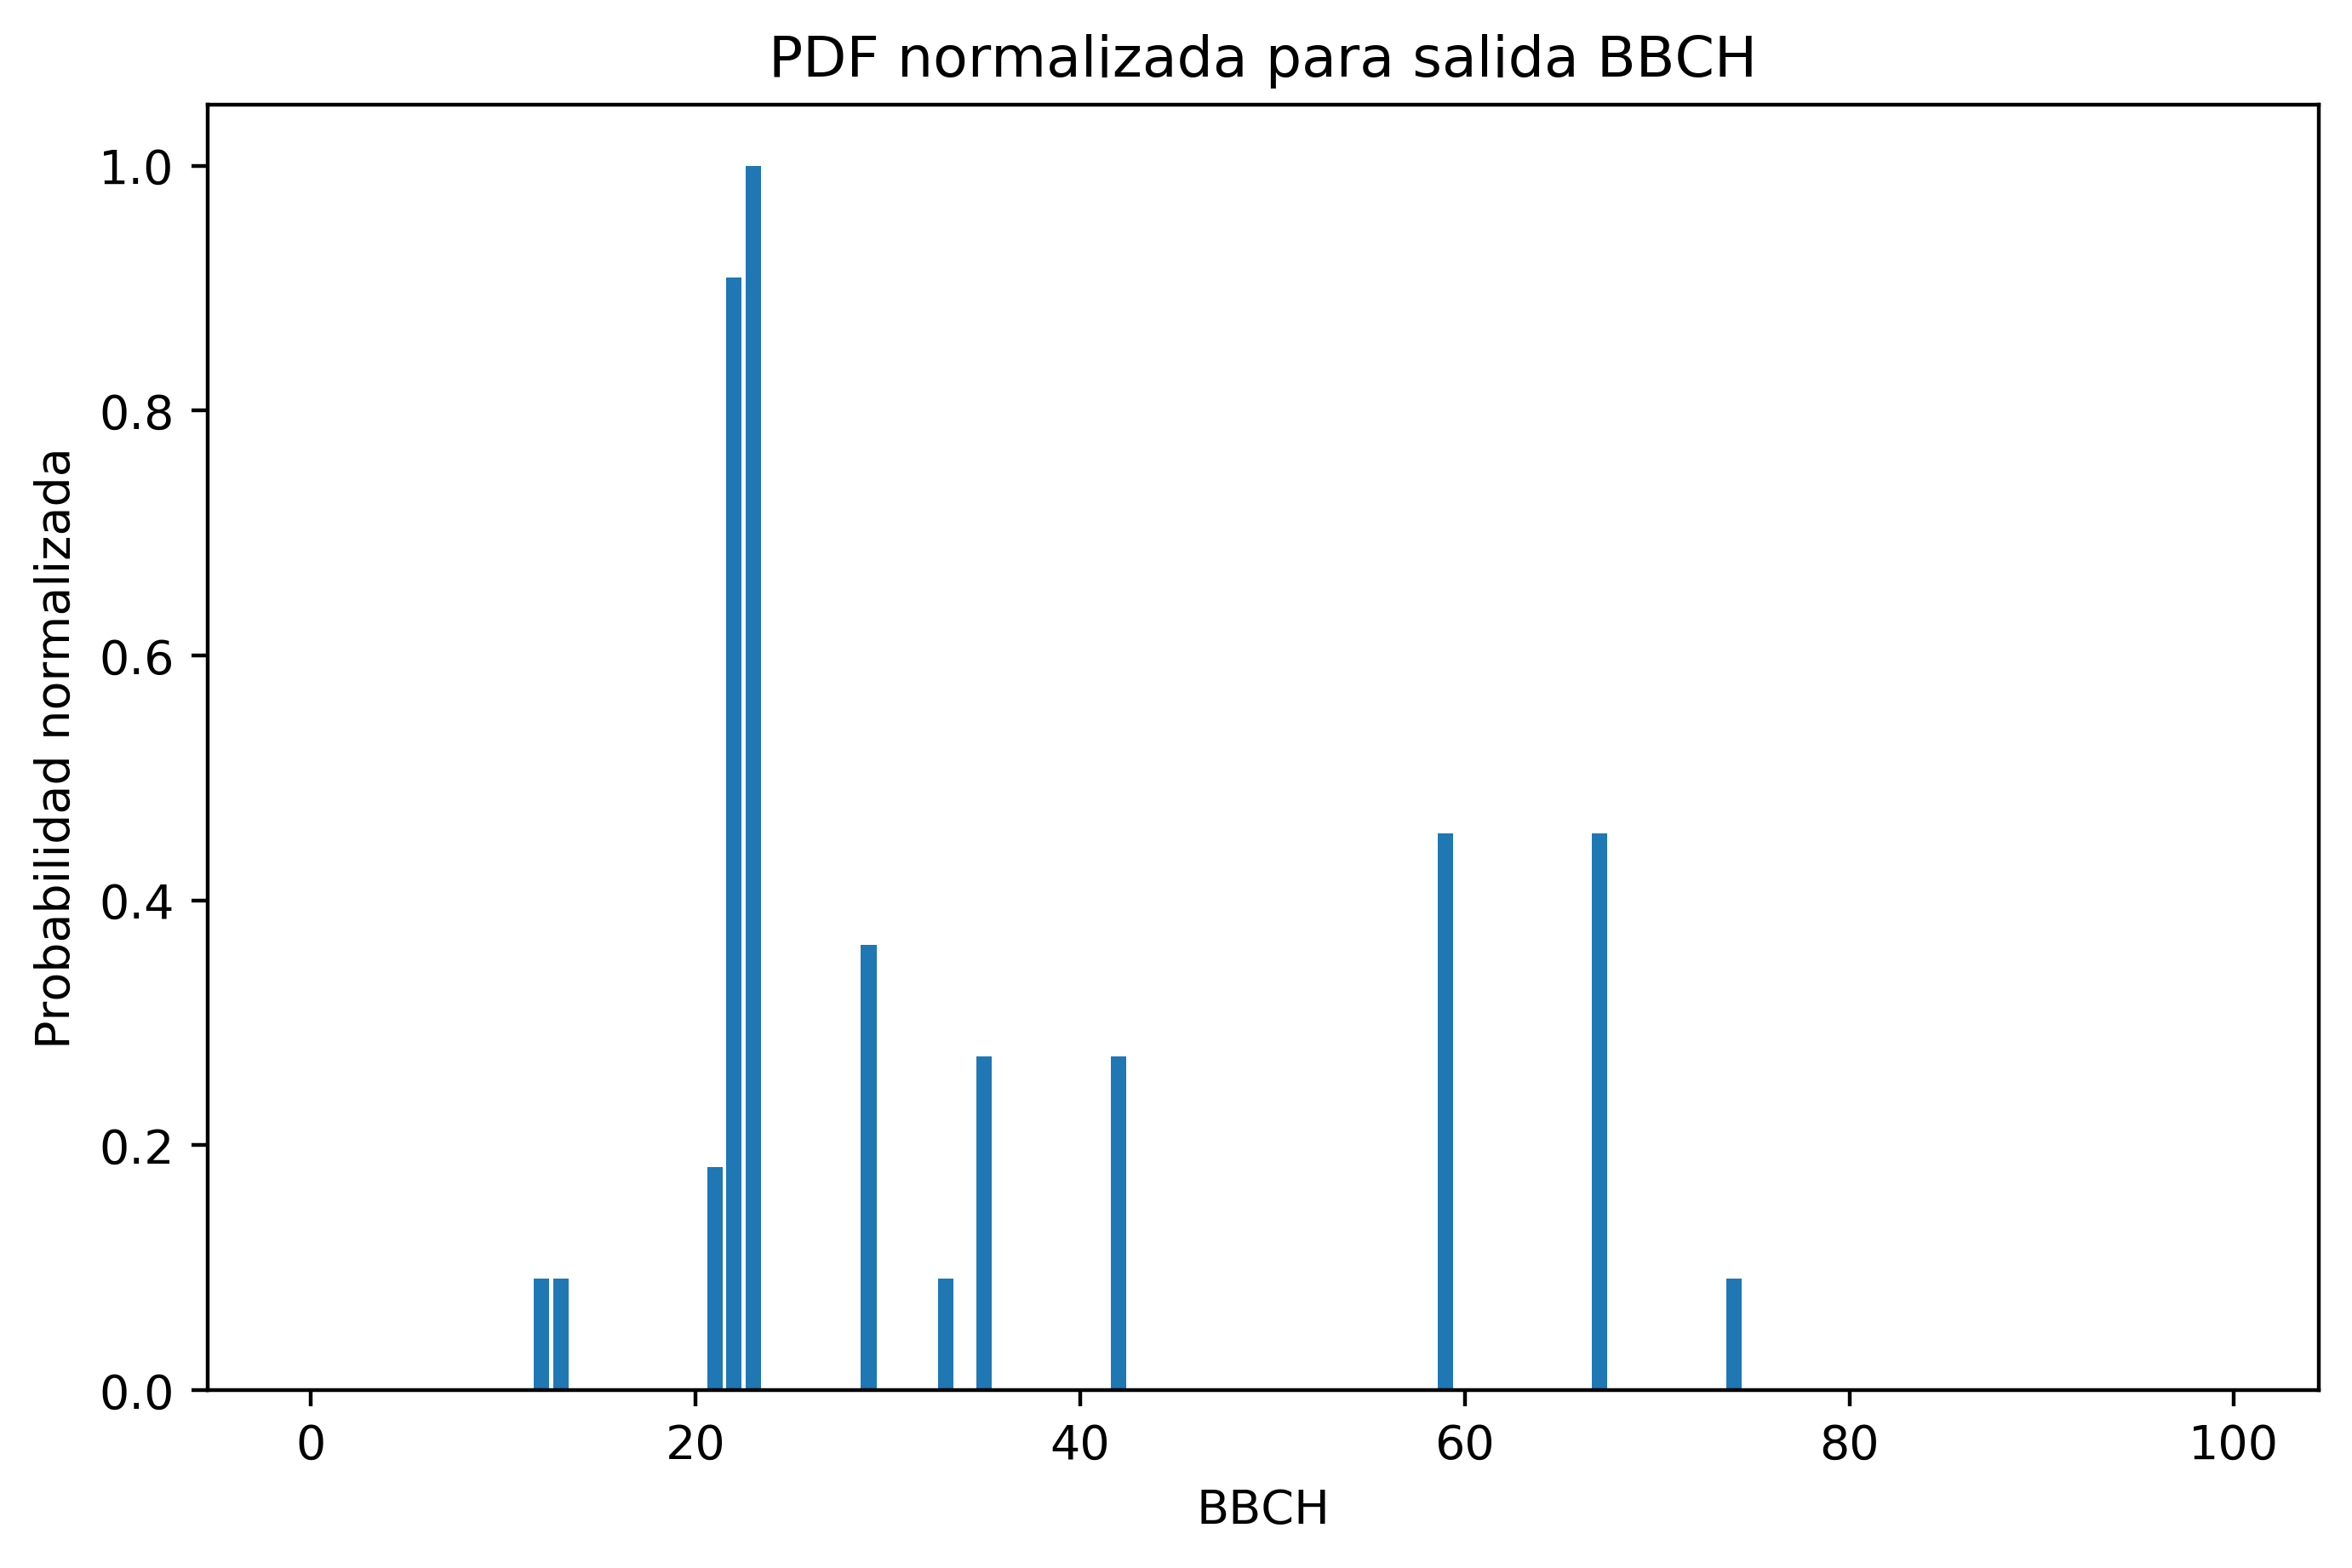
\includegraphics[width=0.95\linewidth]{archivos/tfg/Pixel/BBCHH_PDF_BBCH}
  \caption{Ejemplo del modelo de doble salida: \gls{pdf} estimación de \gls{bbch}\label{fig:p_sub1}}
\end{subfigure}
\begin{subfigure}{0.6\textwidth}
  \centering
  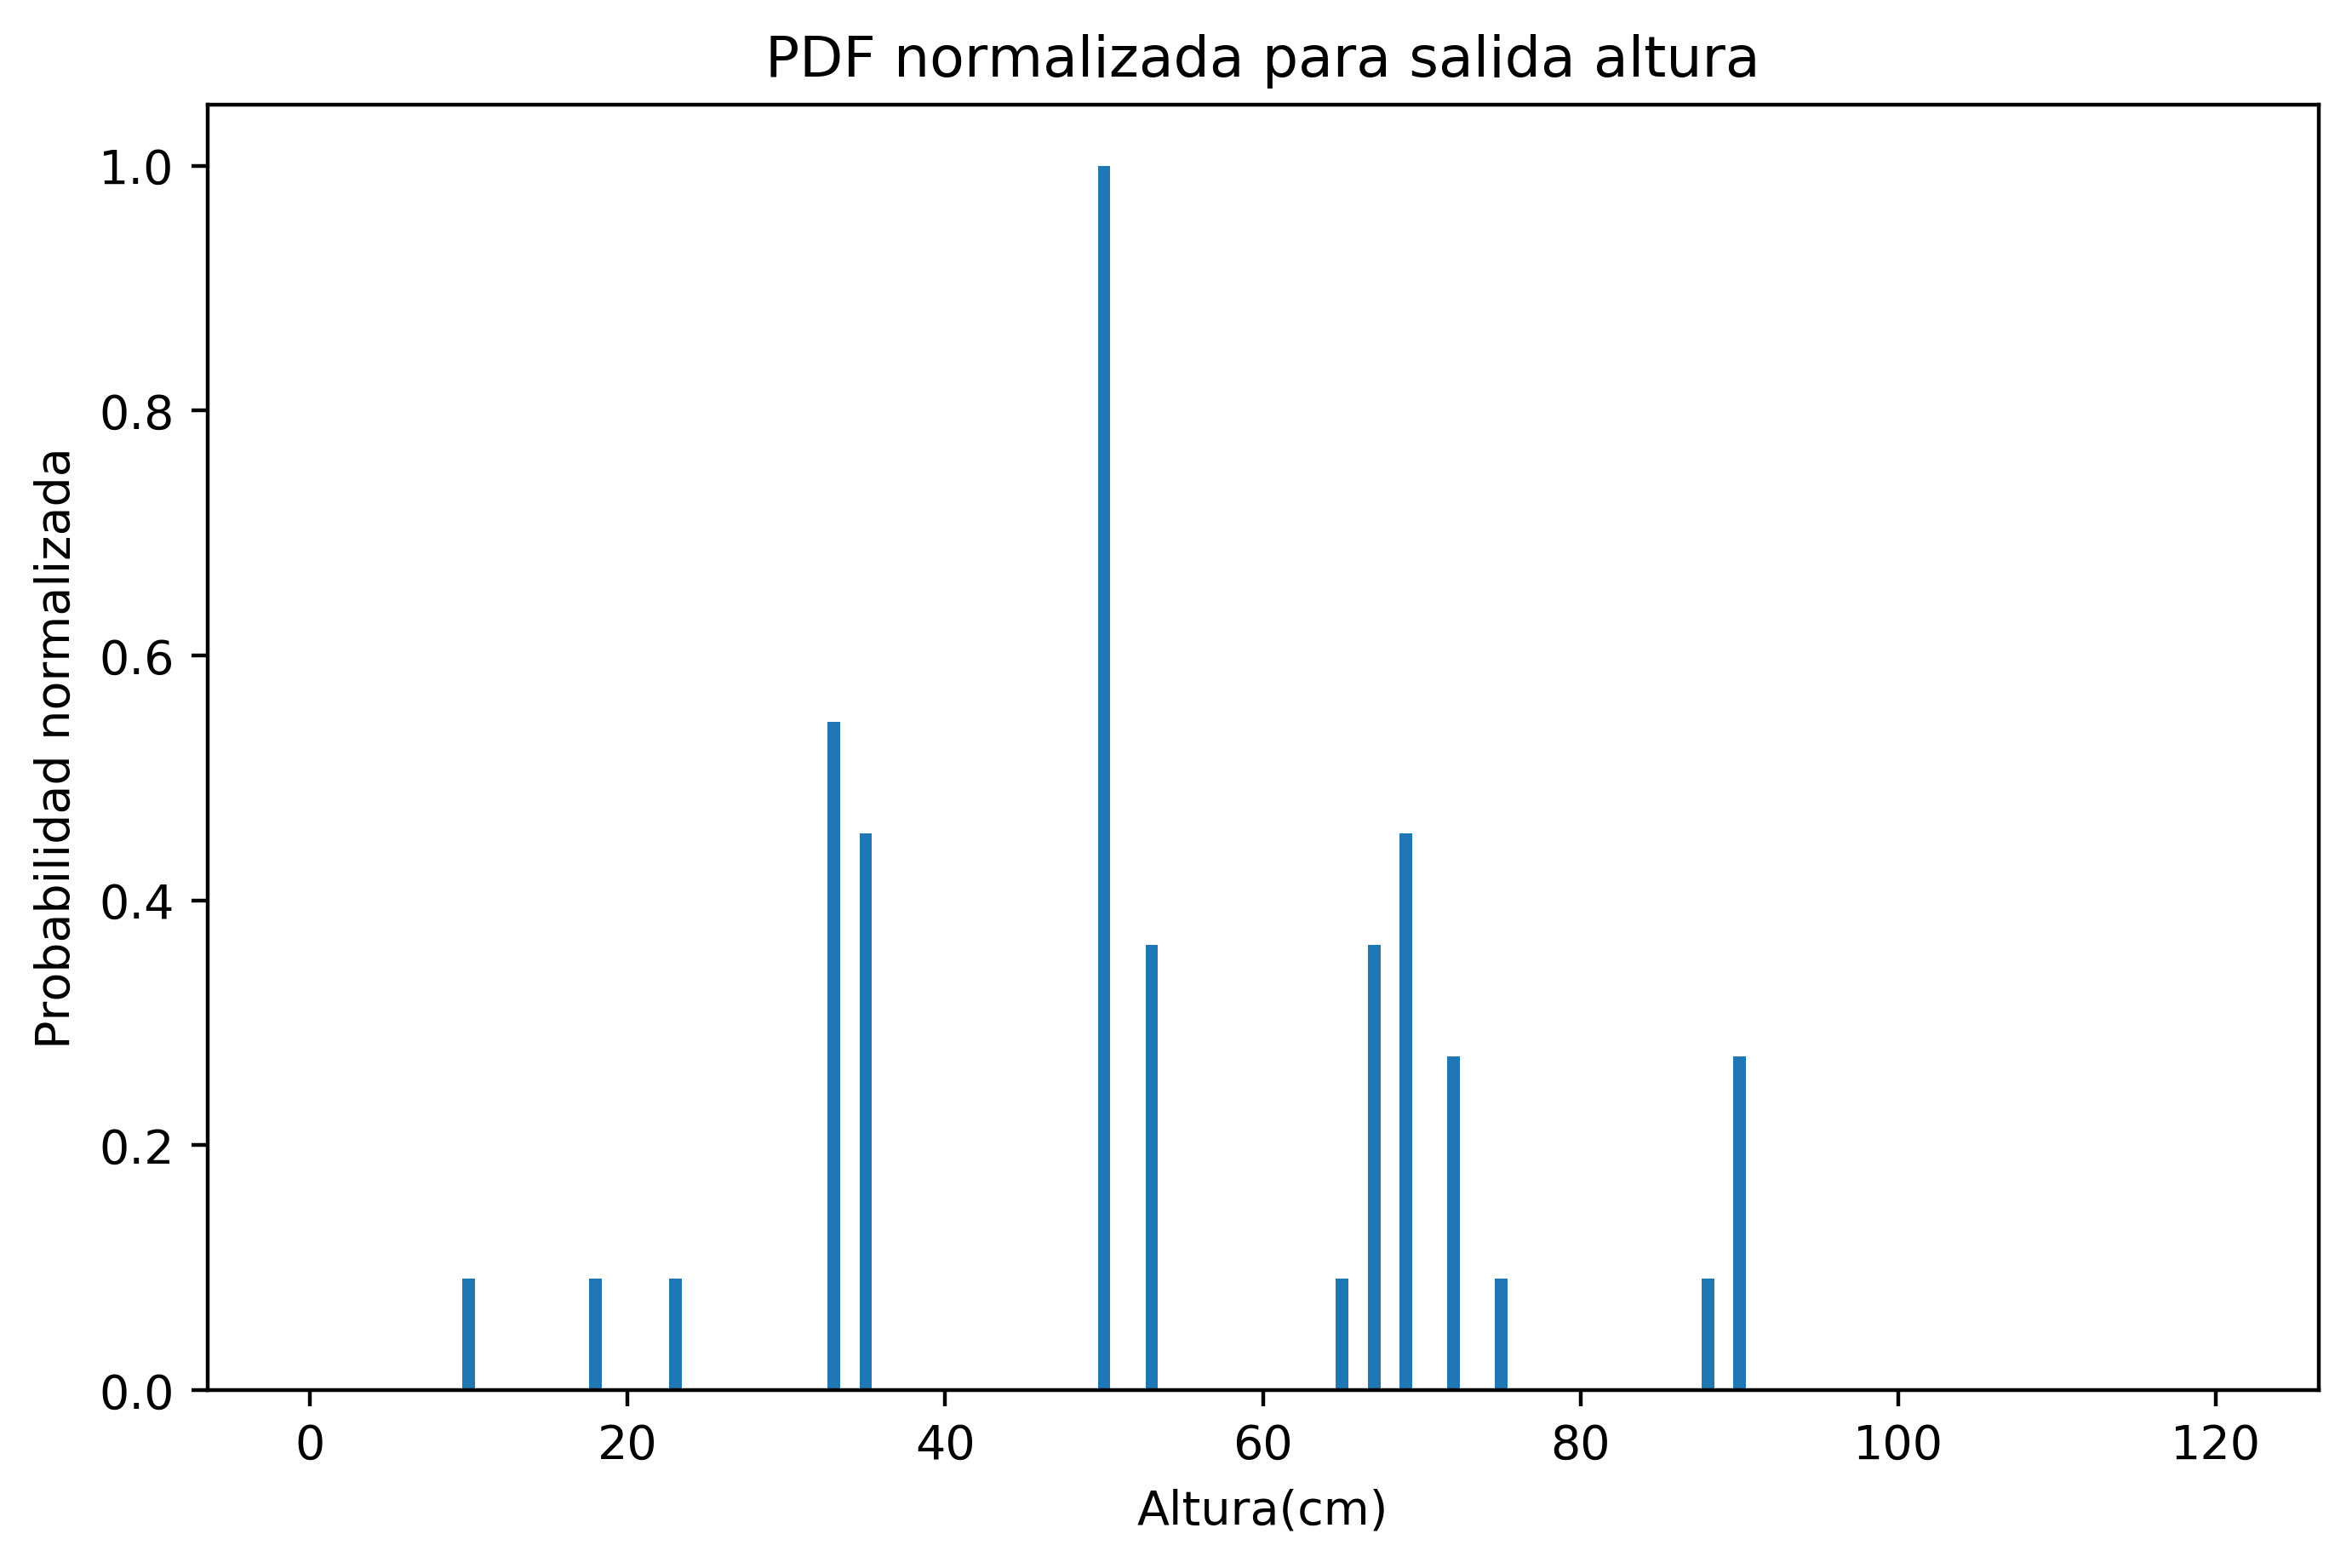
\includegraphics[width=0.95\linewidth]{archivos/tfg/Pixel/BBCHH_PDF_H}
  \caption{Ejemplo del modelo de doble salida: \gls{pdf} estimación de altura\label{fig:p_sub2}}
\end{subfigure}
\caption{Ejemplo de salidas \gls{pdf} normalizadas del modelo para estimación de \gls{bbch} y la altura. \label{fig:p_pdf_bh}}
\end{figure}

\subsubsection{Salidas de valor único}
\par Para continuar con la presentación de los resultados obtenidos, se ilustran en las figuras \ref{fig:p_comp_b}, \ref{fig:p_comp_h} y \ref{fig:p_comp_bh} las comparaciones de las soluciones únicas obtenidas (salida con máxima probabilidad) y los datos de tierra tomados correspondientes para la parcela de test en 2018: \gls{bbch} general, máxima y mínima en la parcela, casos individual (\ref{fig:comp_b}) y de doble salida (\ref{fig:p_sub_c1}), o la altura general del cultivo, también para ambos casos (figuras \ref{fig:p_comp_h} y \ref{fig:p_sub_c2}, respectivamente). Se ha realizado una adaptación en los datos para poder representarlos de esta manera, ya que aquí la estimación de valor único se realiza a nivel de pixel y no de parcela, como los datos para contrastar. Es por ello que, para una representación y comprensión más sencillas, se representa la media y la desviación estándar para los píxeles a nivel de parcela y día. 
\\
\par En este método ambos modelos son comparables para las dos salidas posibles ya que todos ellos comparten la misma parcela de test, por lo que se compara la eficiencia para los mismos datos. Comenzando por los modelos de predicción de \gls{bbch} representados en las figuras \ref{fig:p_comp_b} y \ref{fig:p_sub_c1}, se pueden observar estimaciones y errores de nuevo muy parecidos. Ambos modelos presentan una tendencia creciente, que estima a la baja la fenología para las últimas etapas del desarrollo y los mismos picos de predicción errónea sobre los días desde la siembra de 30-40 ya comentados anteriormente. Exceptuando las últimas etapas, se aprecian medias bastante cercanas a los valores reales, aunque con unas desviaciones estándar muy grandes a partir de los 40 días desde la siembra. Estas desviaciones se deben tanto a diferencias reales en la parcela, áreas con diferente nivel de desarrollo, como a un mal ajuste del modelo ya que en el entrenamiento existían estas diferencias en la misma parcela y se ha considerado el mismo valor de \gls{bbch} por la disponibilidad de datos de verdad de tierra. En esta metodología no aparecen diferencias tan claras entre los dos modelos implementados, ya que eran bastante similares. 
\\
\par Considerando las salidas para la altura, también se puede apreciar la gran similitud que presentan las representaciones comparadas: figuras \ref{fig:p_comp_h} y \ref{fig:p_sub_c2}, dificilmente diferenciables a simple vista. Las coincidencias más obvias son las mencionadas con la estimación de la \gls{bbch}: la tendencia creciente, los picos de predicciones erróneas para las mismas etapas y grandes desviaciones estándar, en este caso, durante todo el proceso. Hay que puntualizar, que las medias para cada parcela tienen valores muy próximos a los reales, sobretodo en las etapas intermedias y finales, cuando la mayoría de los modelos presentan mayor inexactitud. Aunque los resultados globales evaluados para la metodología a nivel de pixel puedan ser numéricamente peores debido a la evaluación independiente de cada pixel, este es el método que mejores resultados ha obtenido para la estimación de la altura.

% Una figura con dos imágenes
\begin{figure}[H]
\centering
\begin{subfigure}{.85\textwidth}
  \centering
  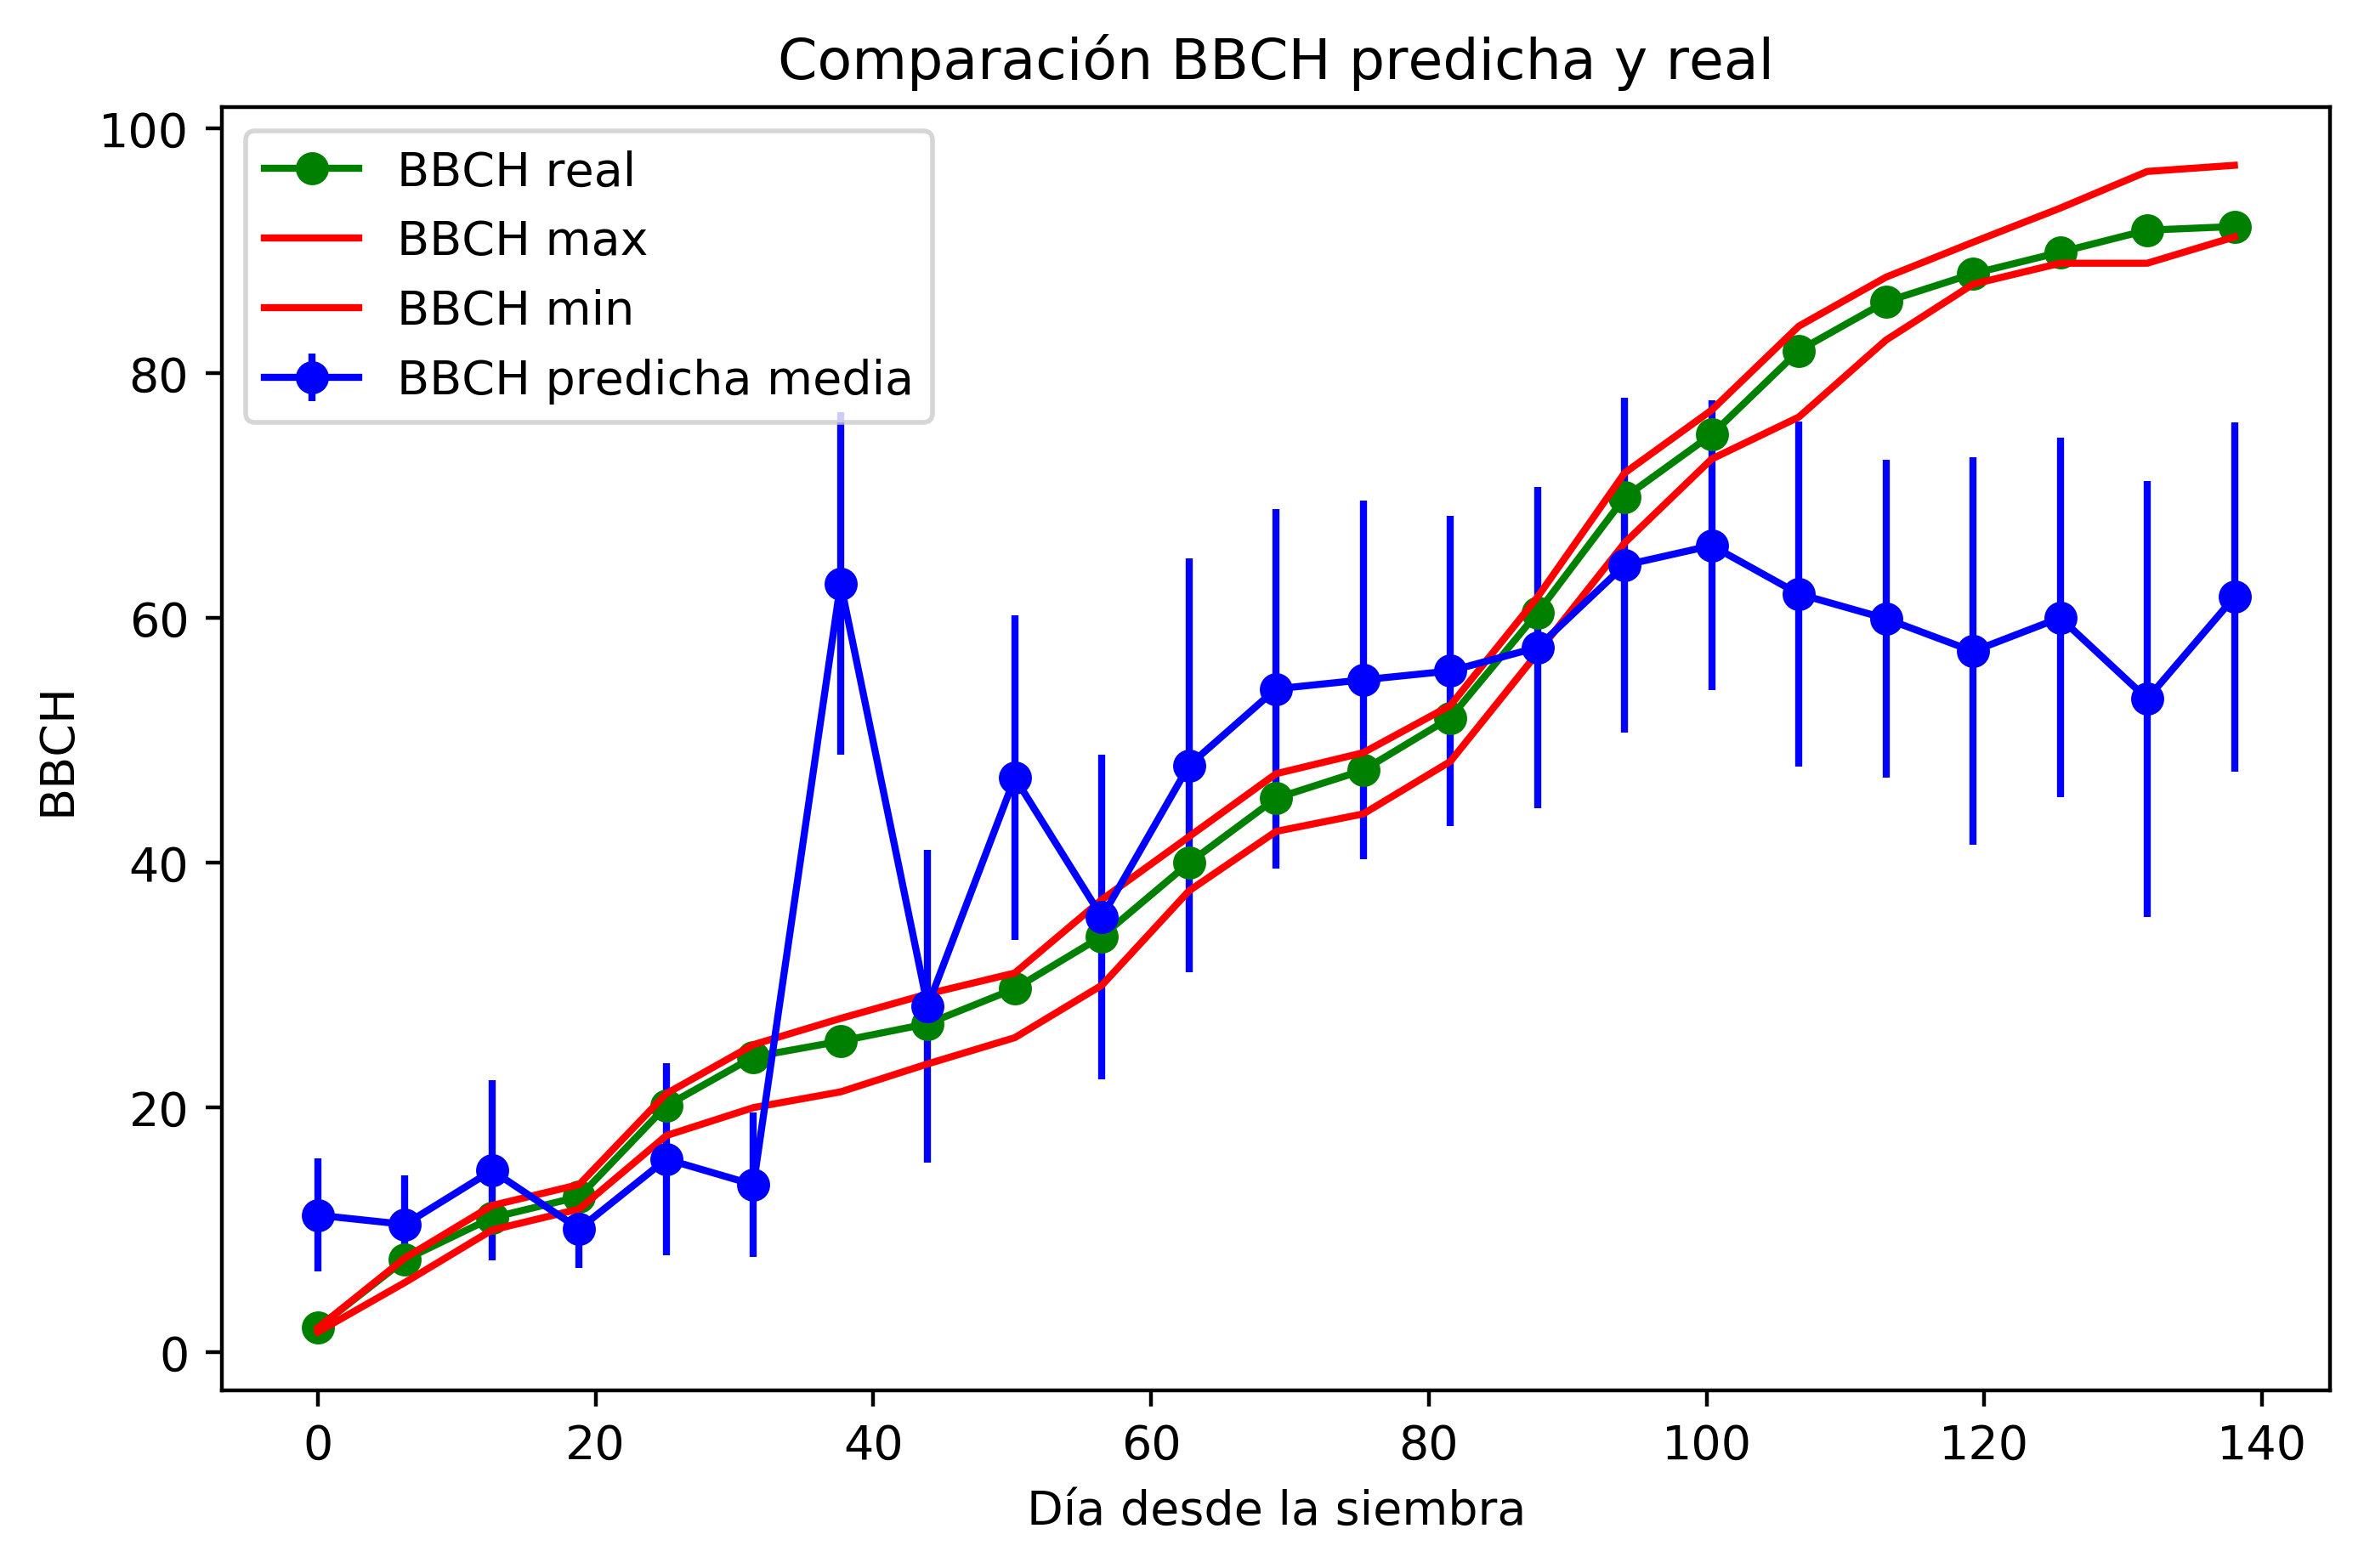
\includegraphics[width=0.95\linewidth]{archivos/tfg/Pixel/BBCH_COMPARACION_BIEN}
  \caption{Comparación de la salida predicha y la verdad de tierra del modelo para estimación de la \gls{bbch}. \label{fig:p_comp_b}}
\end{subfigure}
\begin{subfigure}{.85\textwidth}
  \centering
  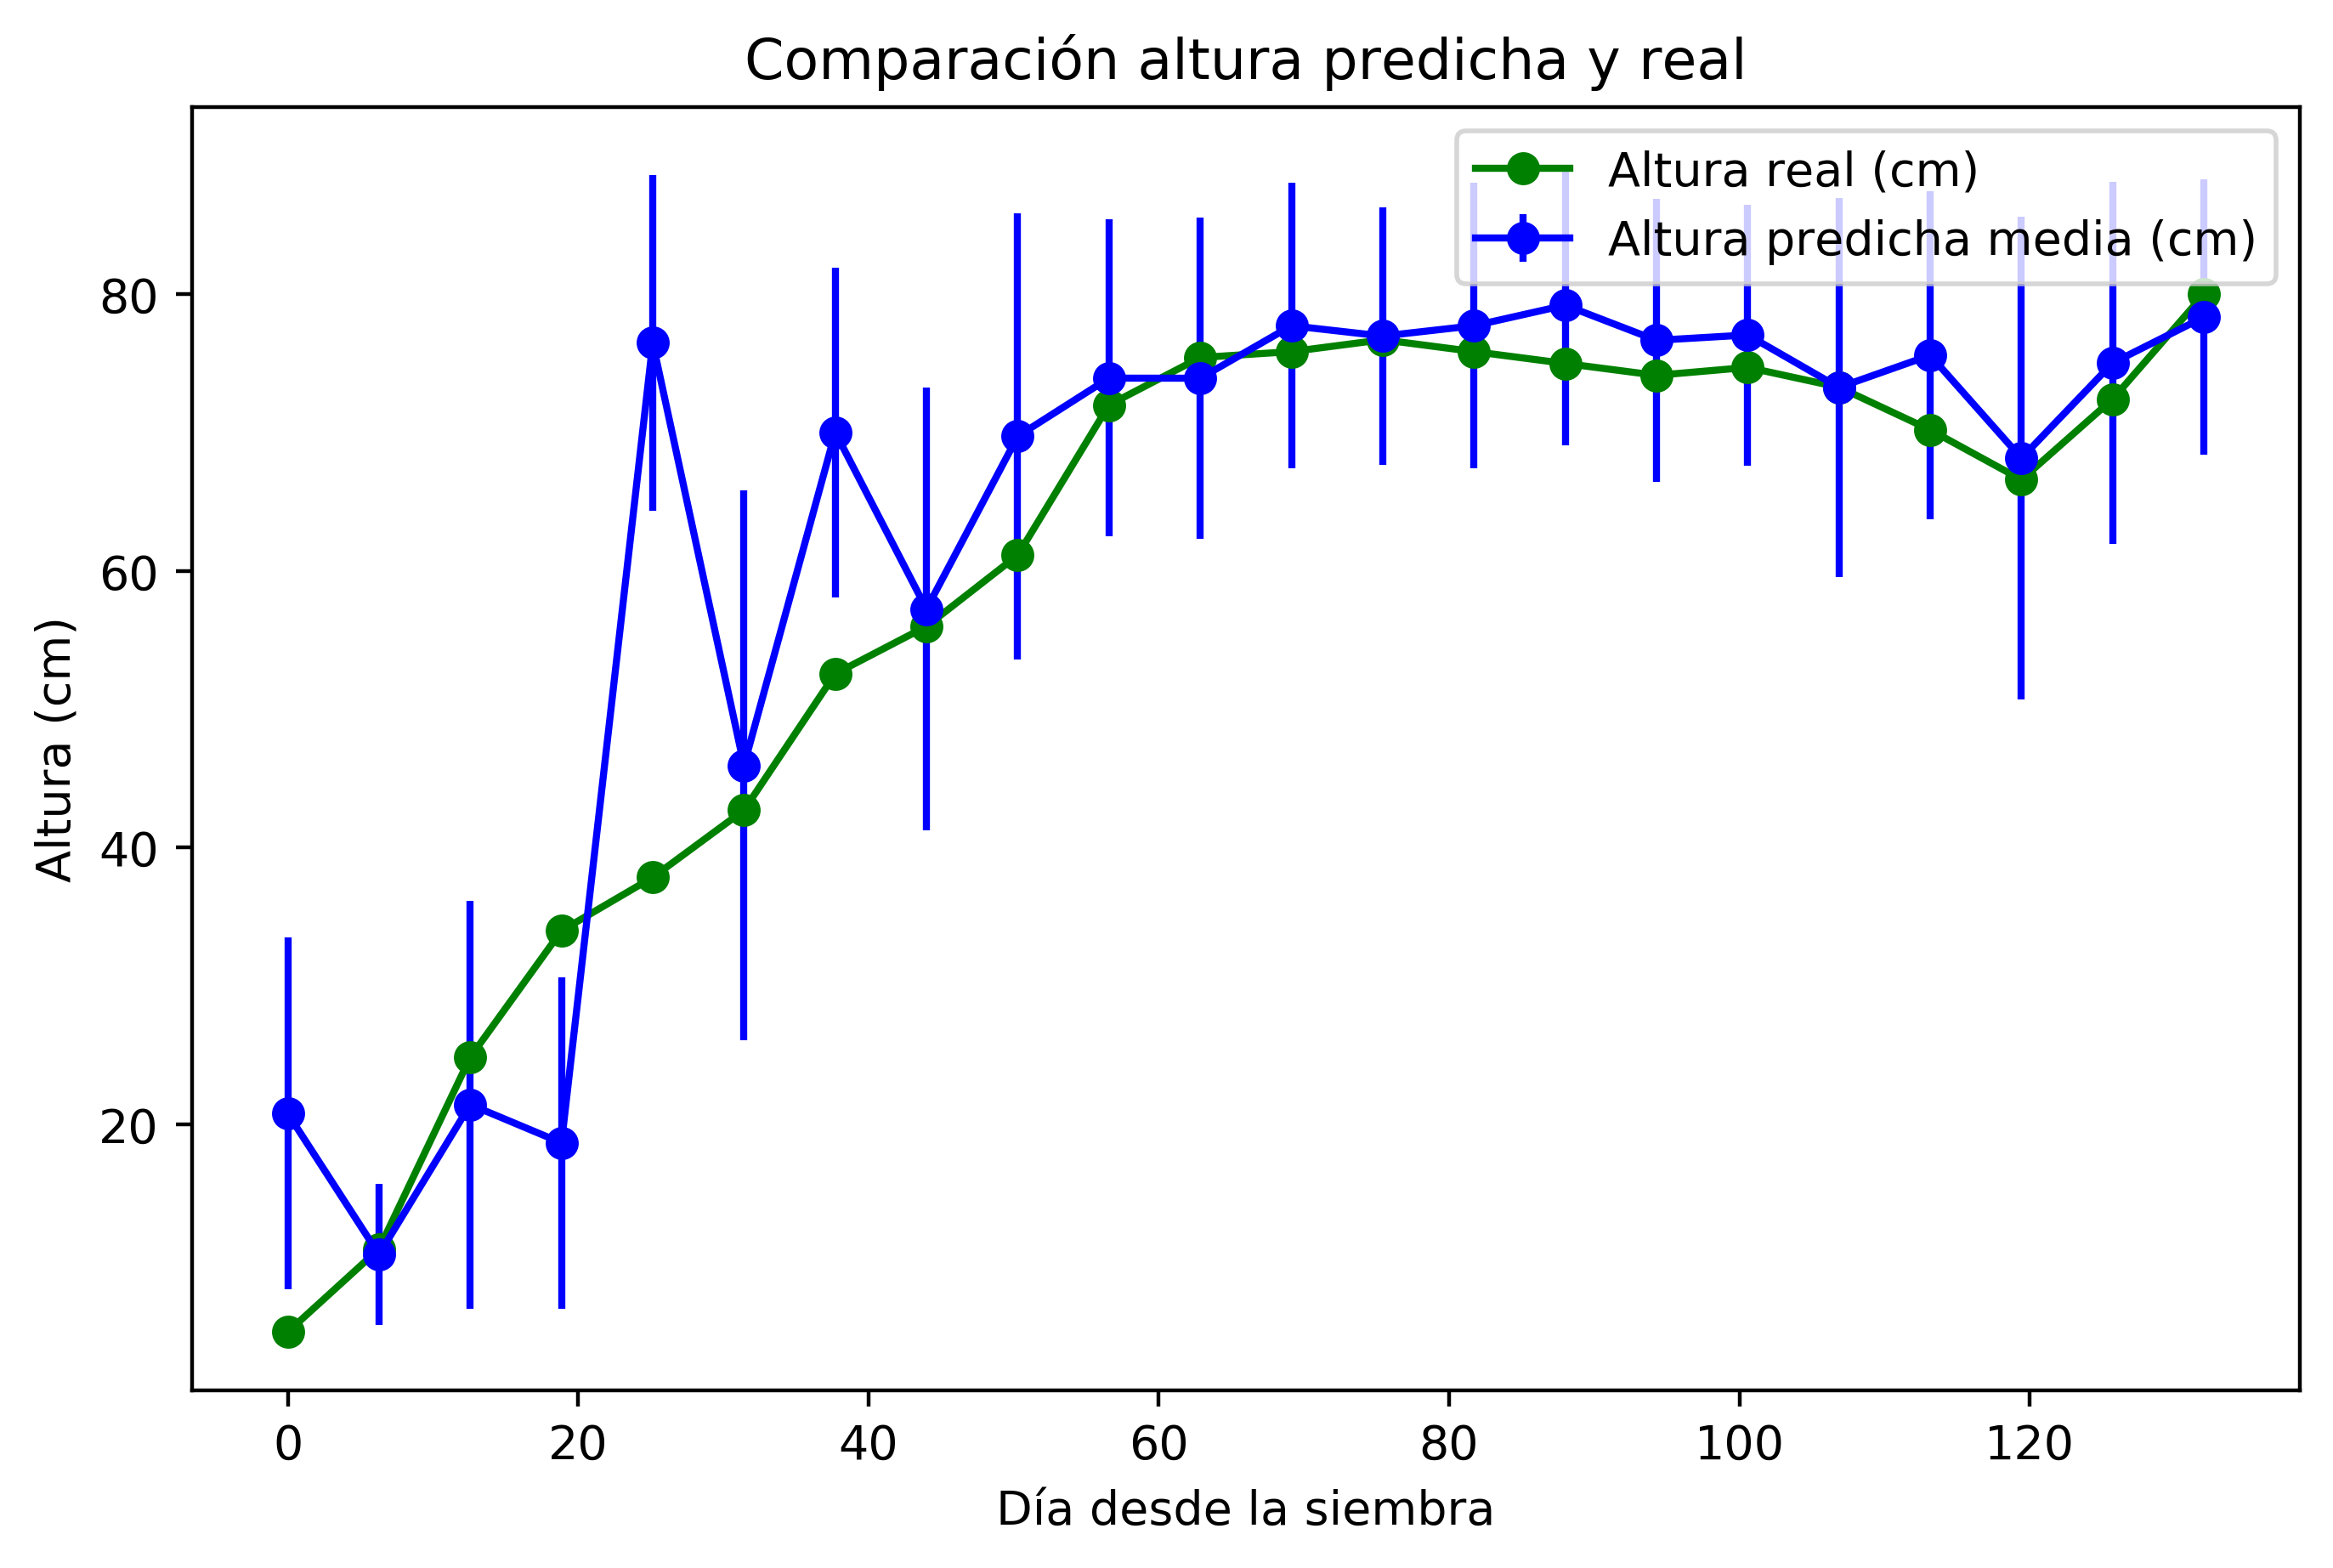
\includegraphics[width=0.95\linewidth]{archivos/tfg/Pixel/H_COMPARACION_BIEN}
  \caption{Comparación de la salida predicha y la verdad de tierra del modelo de doble salida para la estimación de la altura\label{fig:p_comp_h}}
\end{subfigure}
\caption{Comparación de la salida predicha y la verdad de tierra de los modelos de salidas individuales. \label{fig:p_comp}}
\end{figure}

% Una figura con dos imágenes
\begin{figure}[H]
\centering
\begin{subfigure}{.85\textwidth}
  \centering
  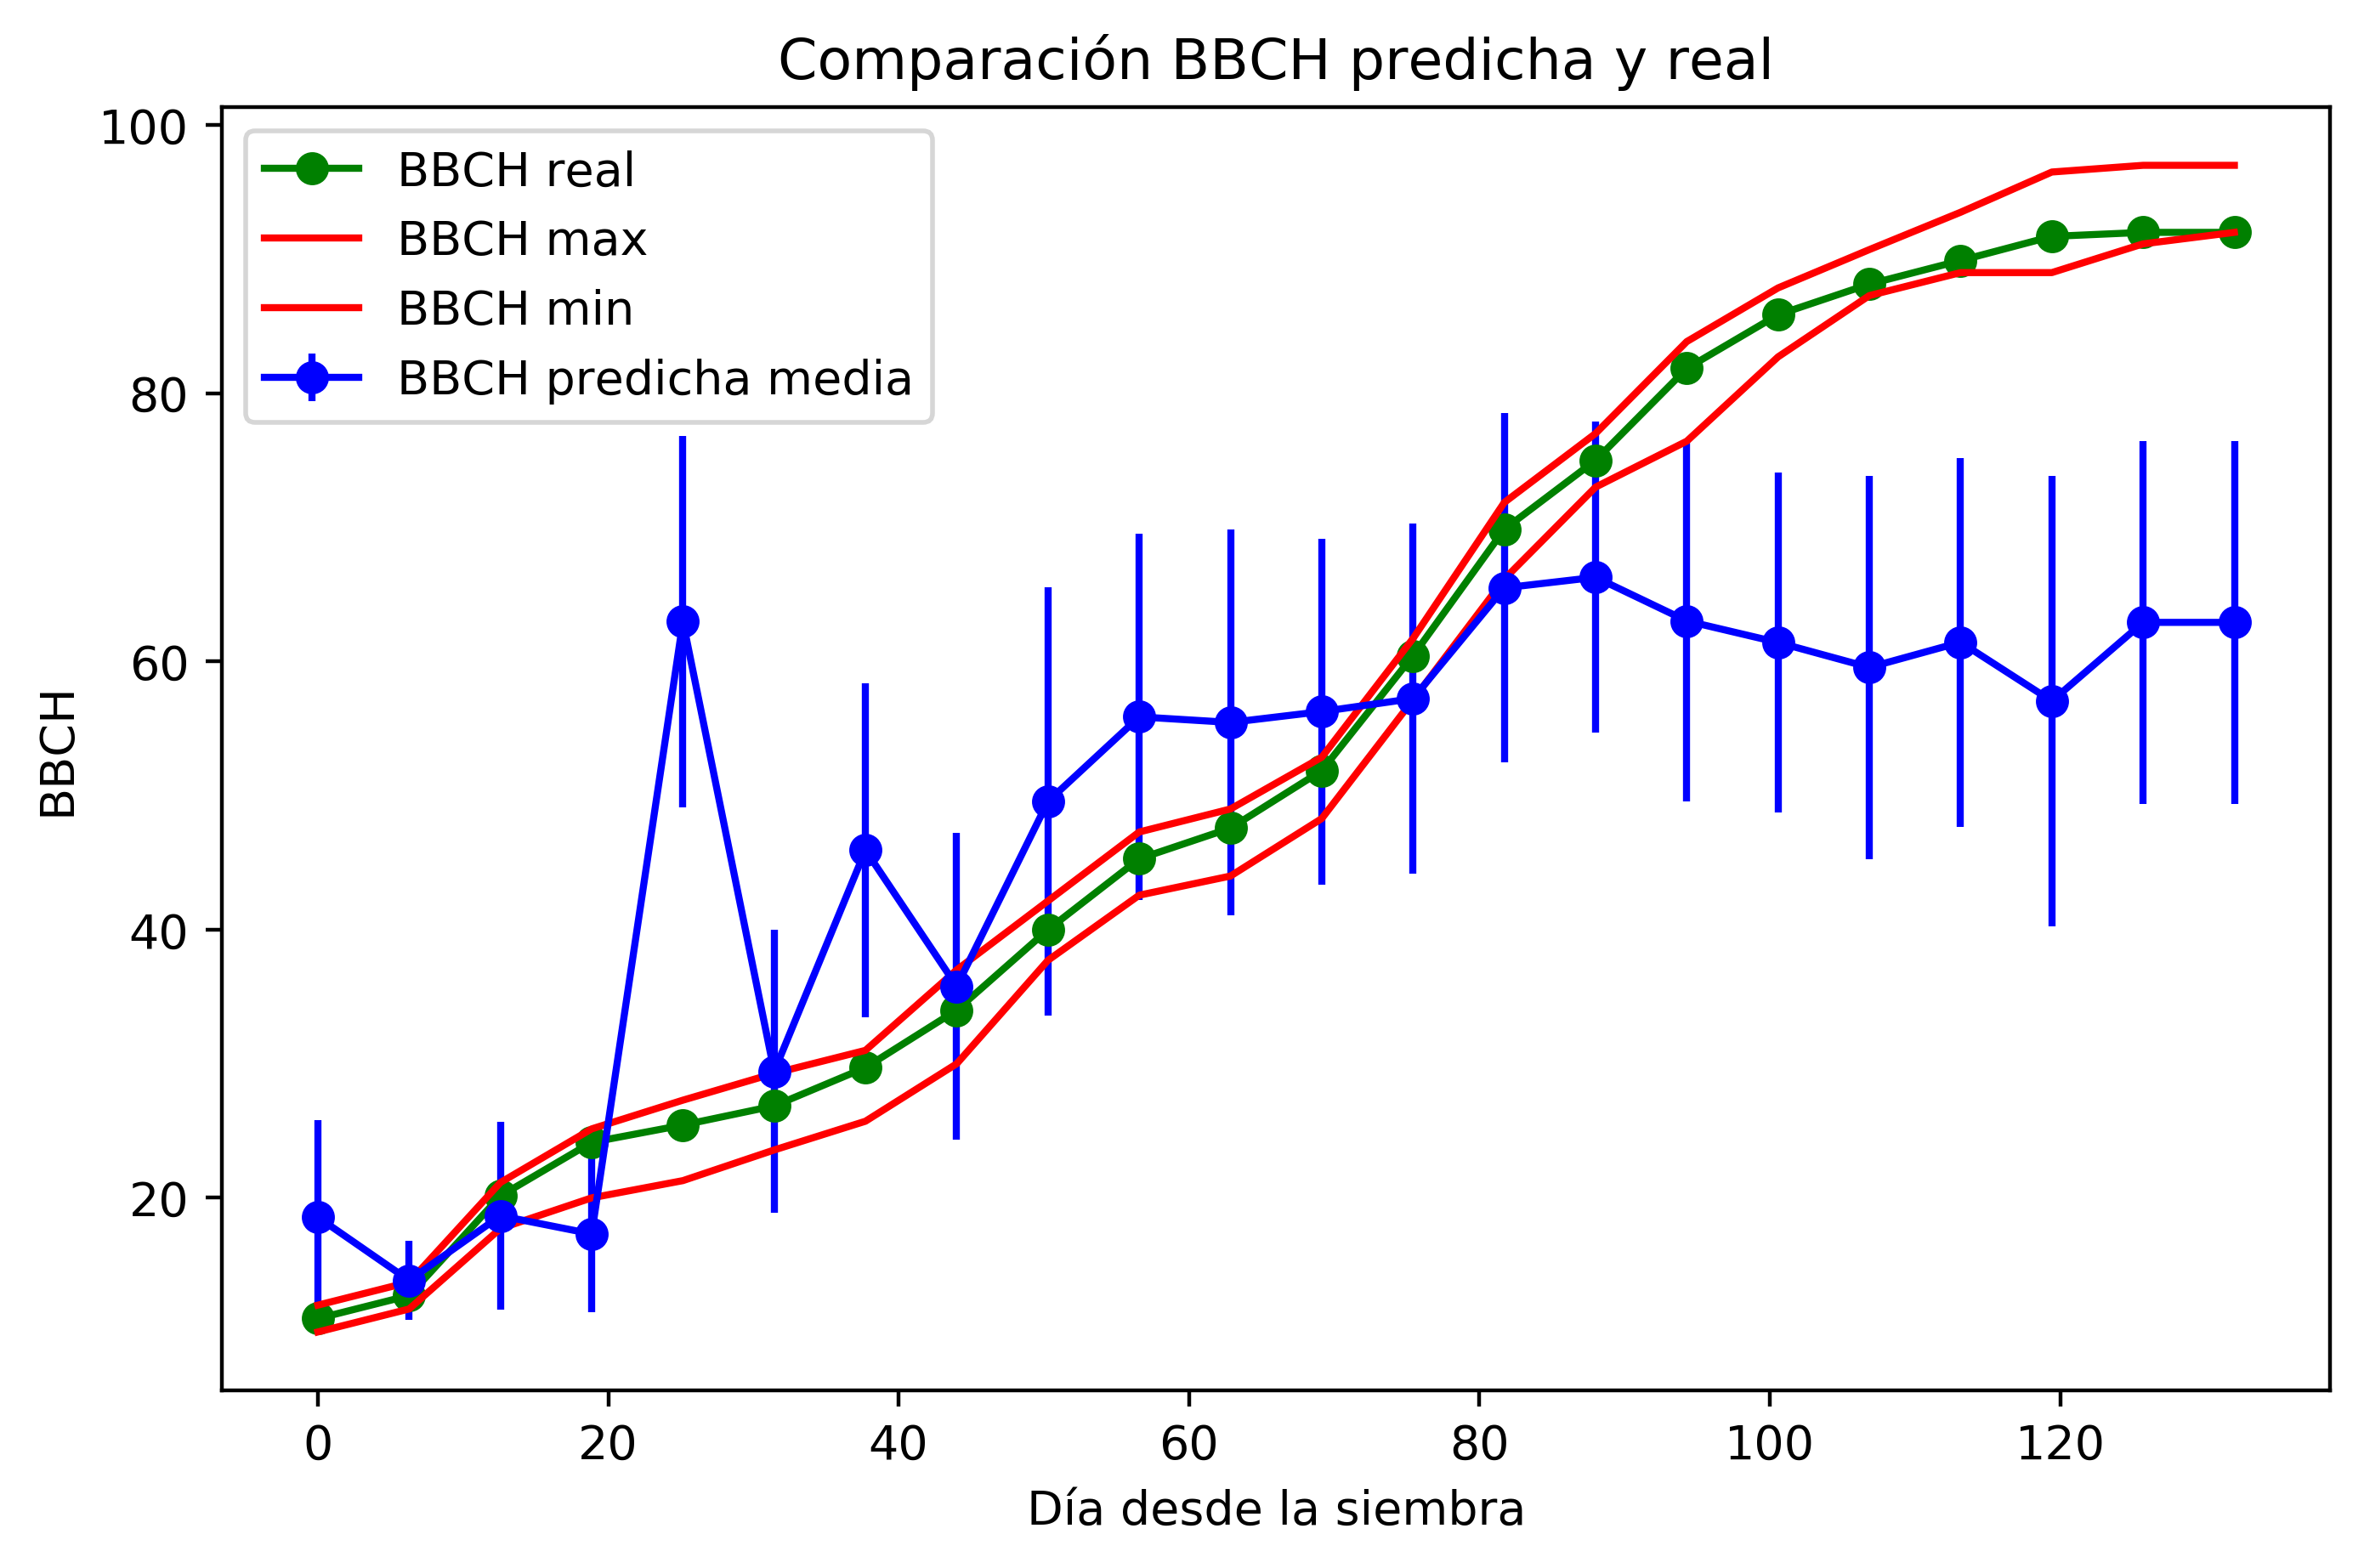
\includegraphics[width=0.95\linewidth]{archivos/tfg/Pixel/BBCHH_COMPARACION_BIEN_BBCH}
  \caption{Comparación de la salida predicha y la verdad de tierra del modelo de doble salida para la estimación de \gls{bbch}. \label{fig:p_sub_c1}}
\end{subfigure}

\begin{subfigure}{.85\textwidth}
  \centering
  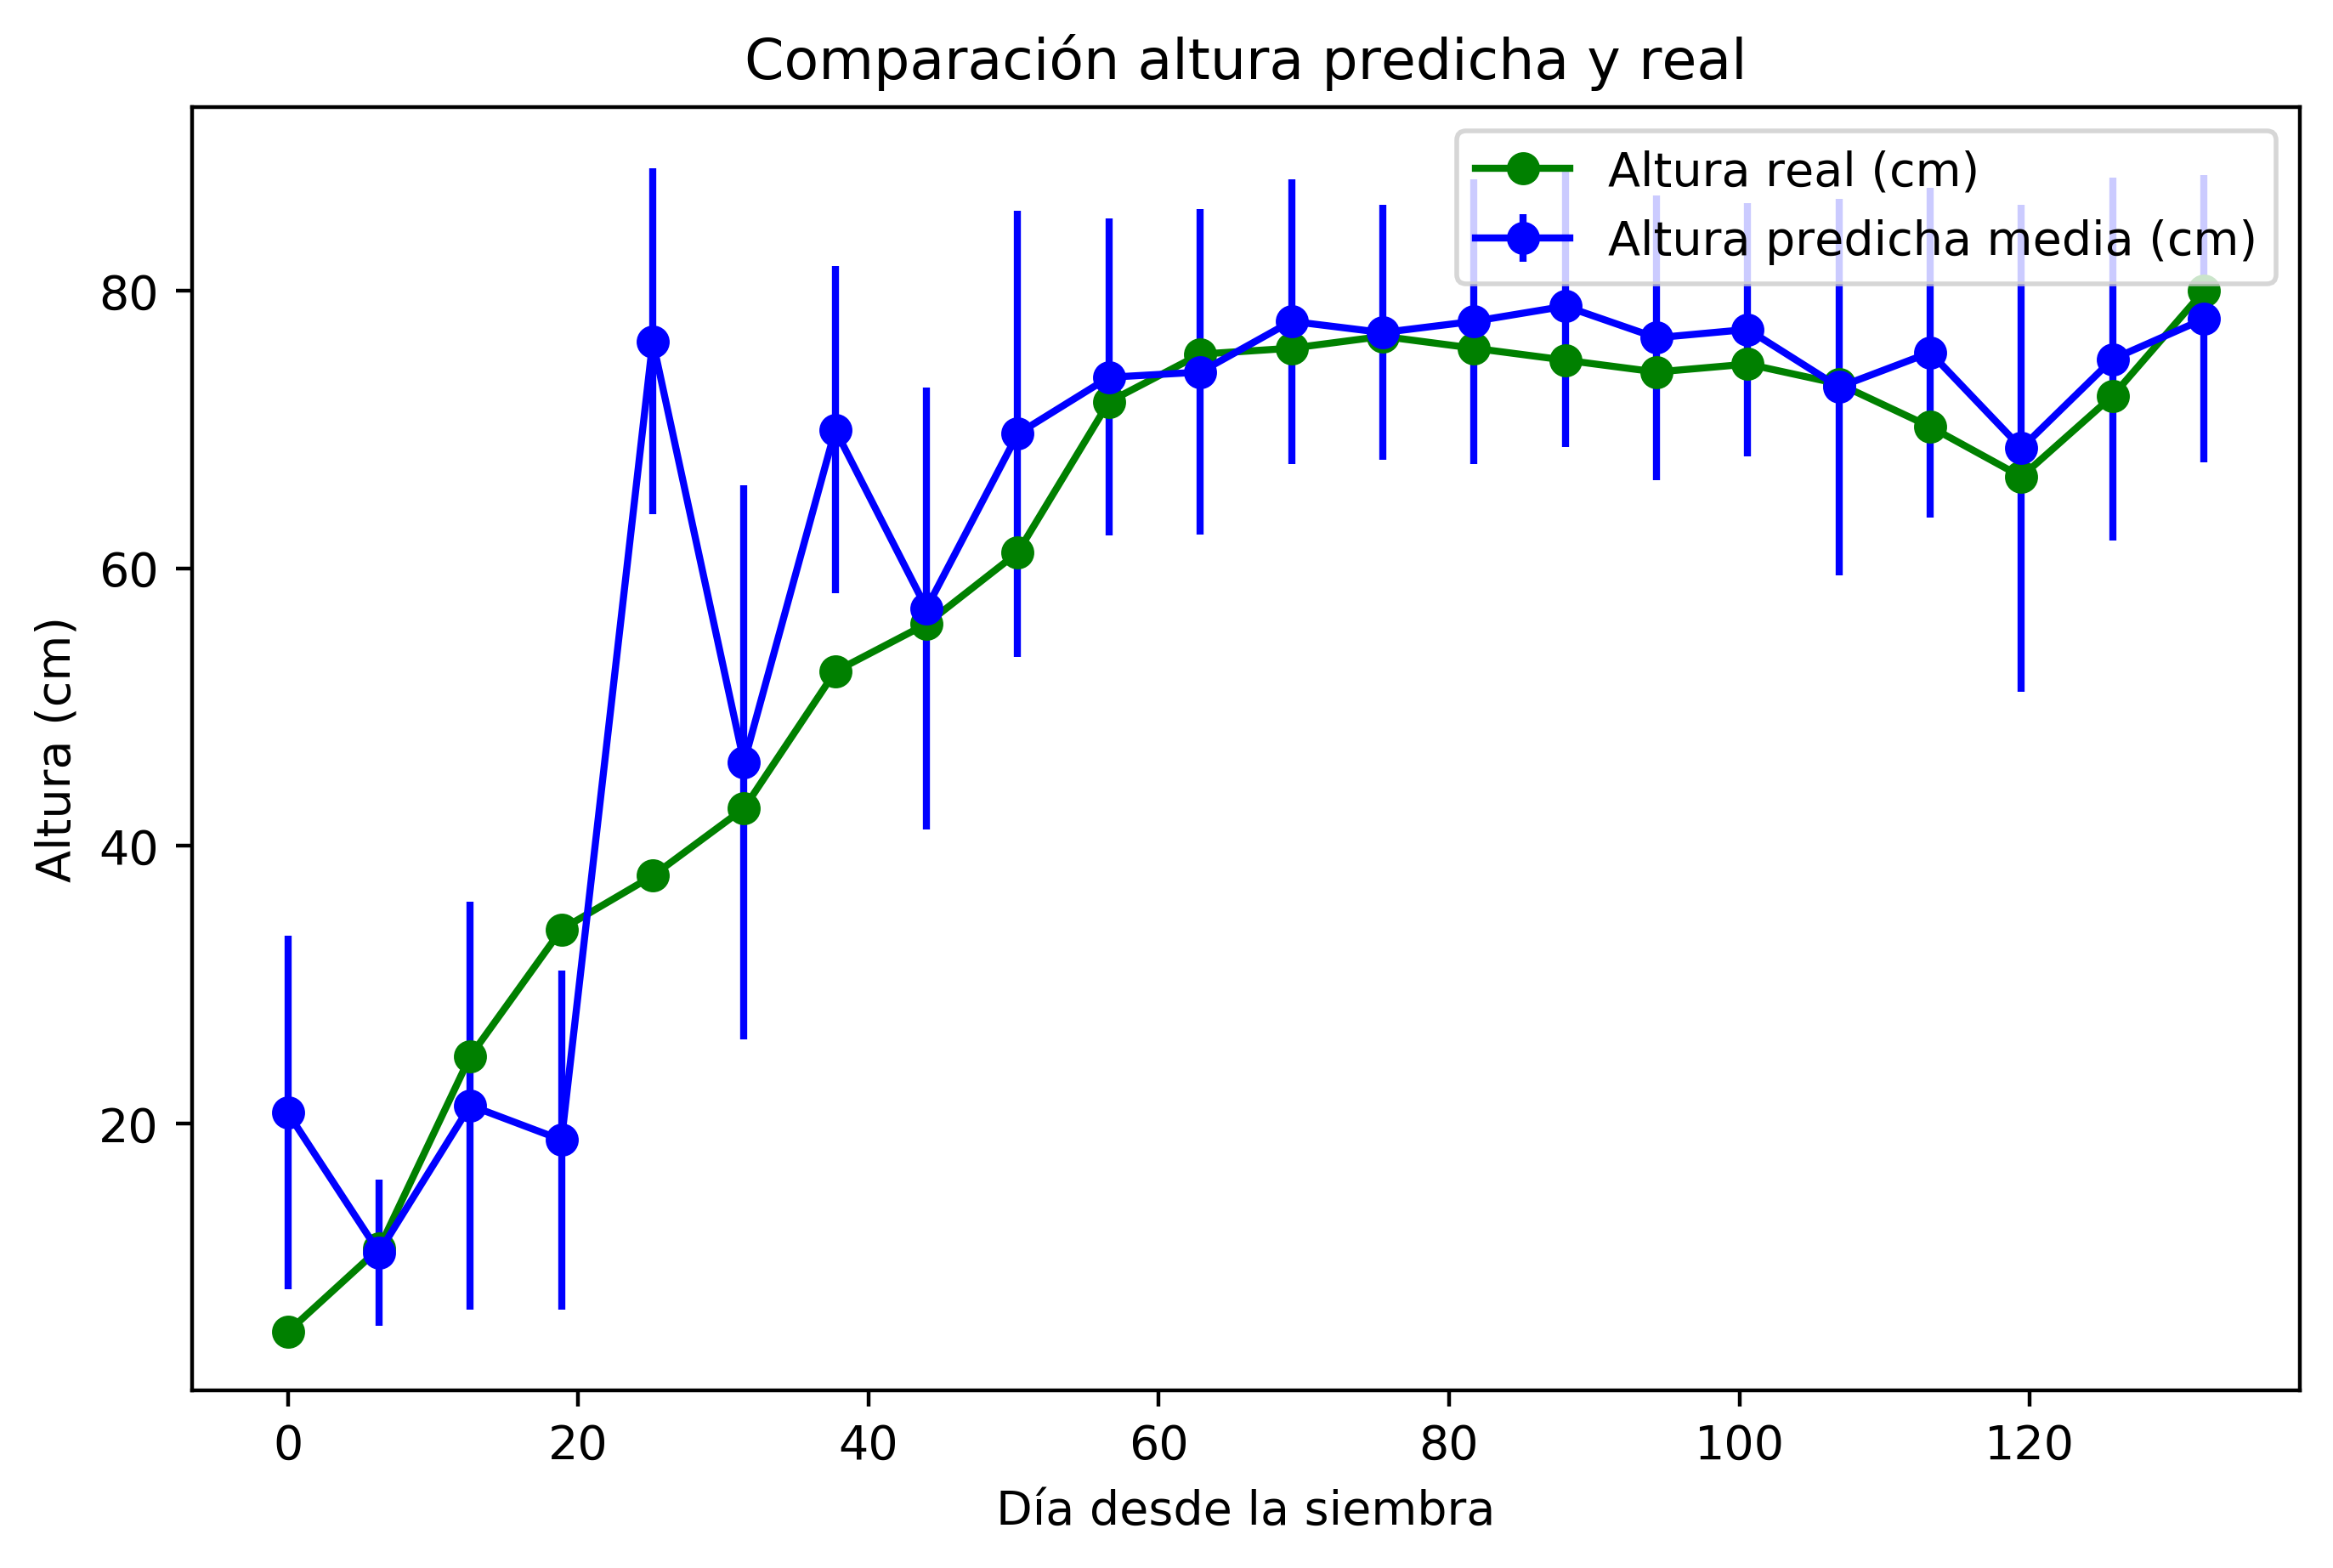
\includegraphics[width=0.95\linewidth]{archivos/tfg/Pixel/BBCHH_COMPARACION_BIEN_H}
  \caption{Comparación de la salida predicha y la verdad de tierra del modelo de doble salida para la estimación de la altura\label{fig:p_sub_c2}}
\end{subfigure}
\caption{Comparación de la salida predicha y la verdad de tierra del modelo de doble salida para la estimación de \gls{bbch} y la altura. \label{fig:p_comp_bh}}
\end{figure}

\subsection{Evaluación de resultados}
\par Para la evaluación de los resultados obtenidos para el método por píxeles se van a utilizar, como se ha mencionado anteriormente, las salidas de valor único por su facilidad para ser representadas y comparadas con los valores únicos medidos. 
\\
\par La primera evaluación realizada se basa en la relación directa entre las salidas estimadas medias por día y las medidas reales, lo cuál muestra la fiabilidad del modelo de una forma más clara y así puede verse en las figuras \ref{fig:p_rel_b}, para el modelo de única salida de \gls{bbch}, \ref{fig:p_rel_h}, para el modelo de única salida de altura y la figura \ref{fig:p_rel_bh} para el modelo de doble salida. En estas representaciones se añade, además, una recta de pendiente ($m$) unidad, la cual sirve de referencia ya que esa relación representaría un modelo ideal. Se han utilizado para todas las representaciones los valores contrastados de la parcela de test correspondiente a cada caso, teniendo en cuenta ambos años de datos, 2017 y 2018.
\\
\par En la figura \ref{fig:p_rel_b} se aprecia una distribución uniforme, lo cuál indica que se disponen de datos suficientes para cubrir las distintas etapas del desarrollo del cultivo. Además, las nubes de puntos se mantienen, en general, cercanos a la recta de referencia, por lo que, excepto para puntos concretos como el pico de las etapas tempranas y las últimas etapas del cultivo, se obtienen resultados bastante buenos. Comparando esta información con la obtenida para el modelo de dos salidas, representado en la figura \ref{fig:p_rel_bh_b}, se puede asegurar a simple vista qué modelo da mejores resultados. En esta última figura las nubes de puntos se presentan más dispersas que en el anterior, aunque siguiendo la tendencia de la recta de referencia. Vemos, contrariamente, agrupaciones de puntos y huecos, por lo que algunas etapas no están siendo estimadas correctamente. Esto se puede deber al hecho de que el procesamiento de este modelo incluye una etapa de limpieza de datos corruptos que se encuentran en los datos de altura, por lo que en algunas etapas, tanto para la \gls{bbch} como  para la altura, faltan datos que aporten la información completa al sistema. 
\\
\par Comparando a continuación las figuras de los modelos con salida de altura del cultivo, \ref{fig:p_rel_bh} para salida única y \ref{fig:p_rel_bh_h} para salida doble, se observa en ambos una mayor inestabilidad en general debida a la concentración de puntos en algunas etapas. La altura de los cultivos no tiene un crecimiento tan lineal progresivo como la fenología de un cultivo, por lo que, a parte de por la corrección de datos, se encuentran concentraciones de datos debido a la estabilidad de la altura durante distintas etapas. Es por ello que, sobre todo en las etapas finales, hay una mayor concentración de puntos, cuando el arroz se mantiene en altura. Aún así, en la figura \ref{fig:p_rel_bh} se aprecia que todas las estimaciones de altura tienden a la baja para casi todos los datos de altura mayor a 80cm. Una posible explicación sería una tendencia generalizada más baja en las parcelas utilizadas para entrenar el modelo o la poca variación en los parámetros de entrada para alturas desde 50cm hasta 110cm, intervalo en el que la altura estimada se mantiene en torno a la misma franja de valores. 

\begin{figure}[H]
\centering
\begin{subfigure}{.7\textwidth}
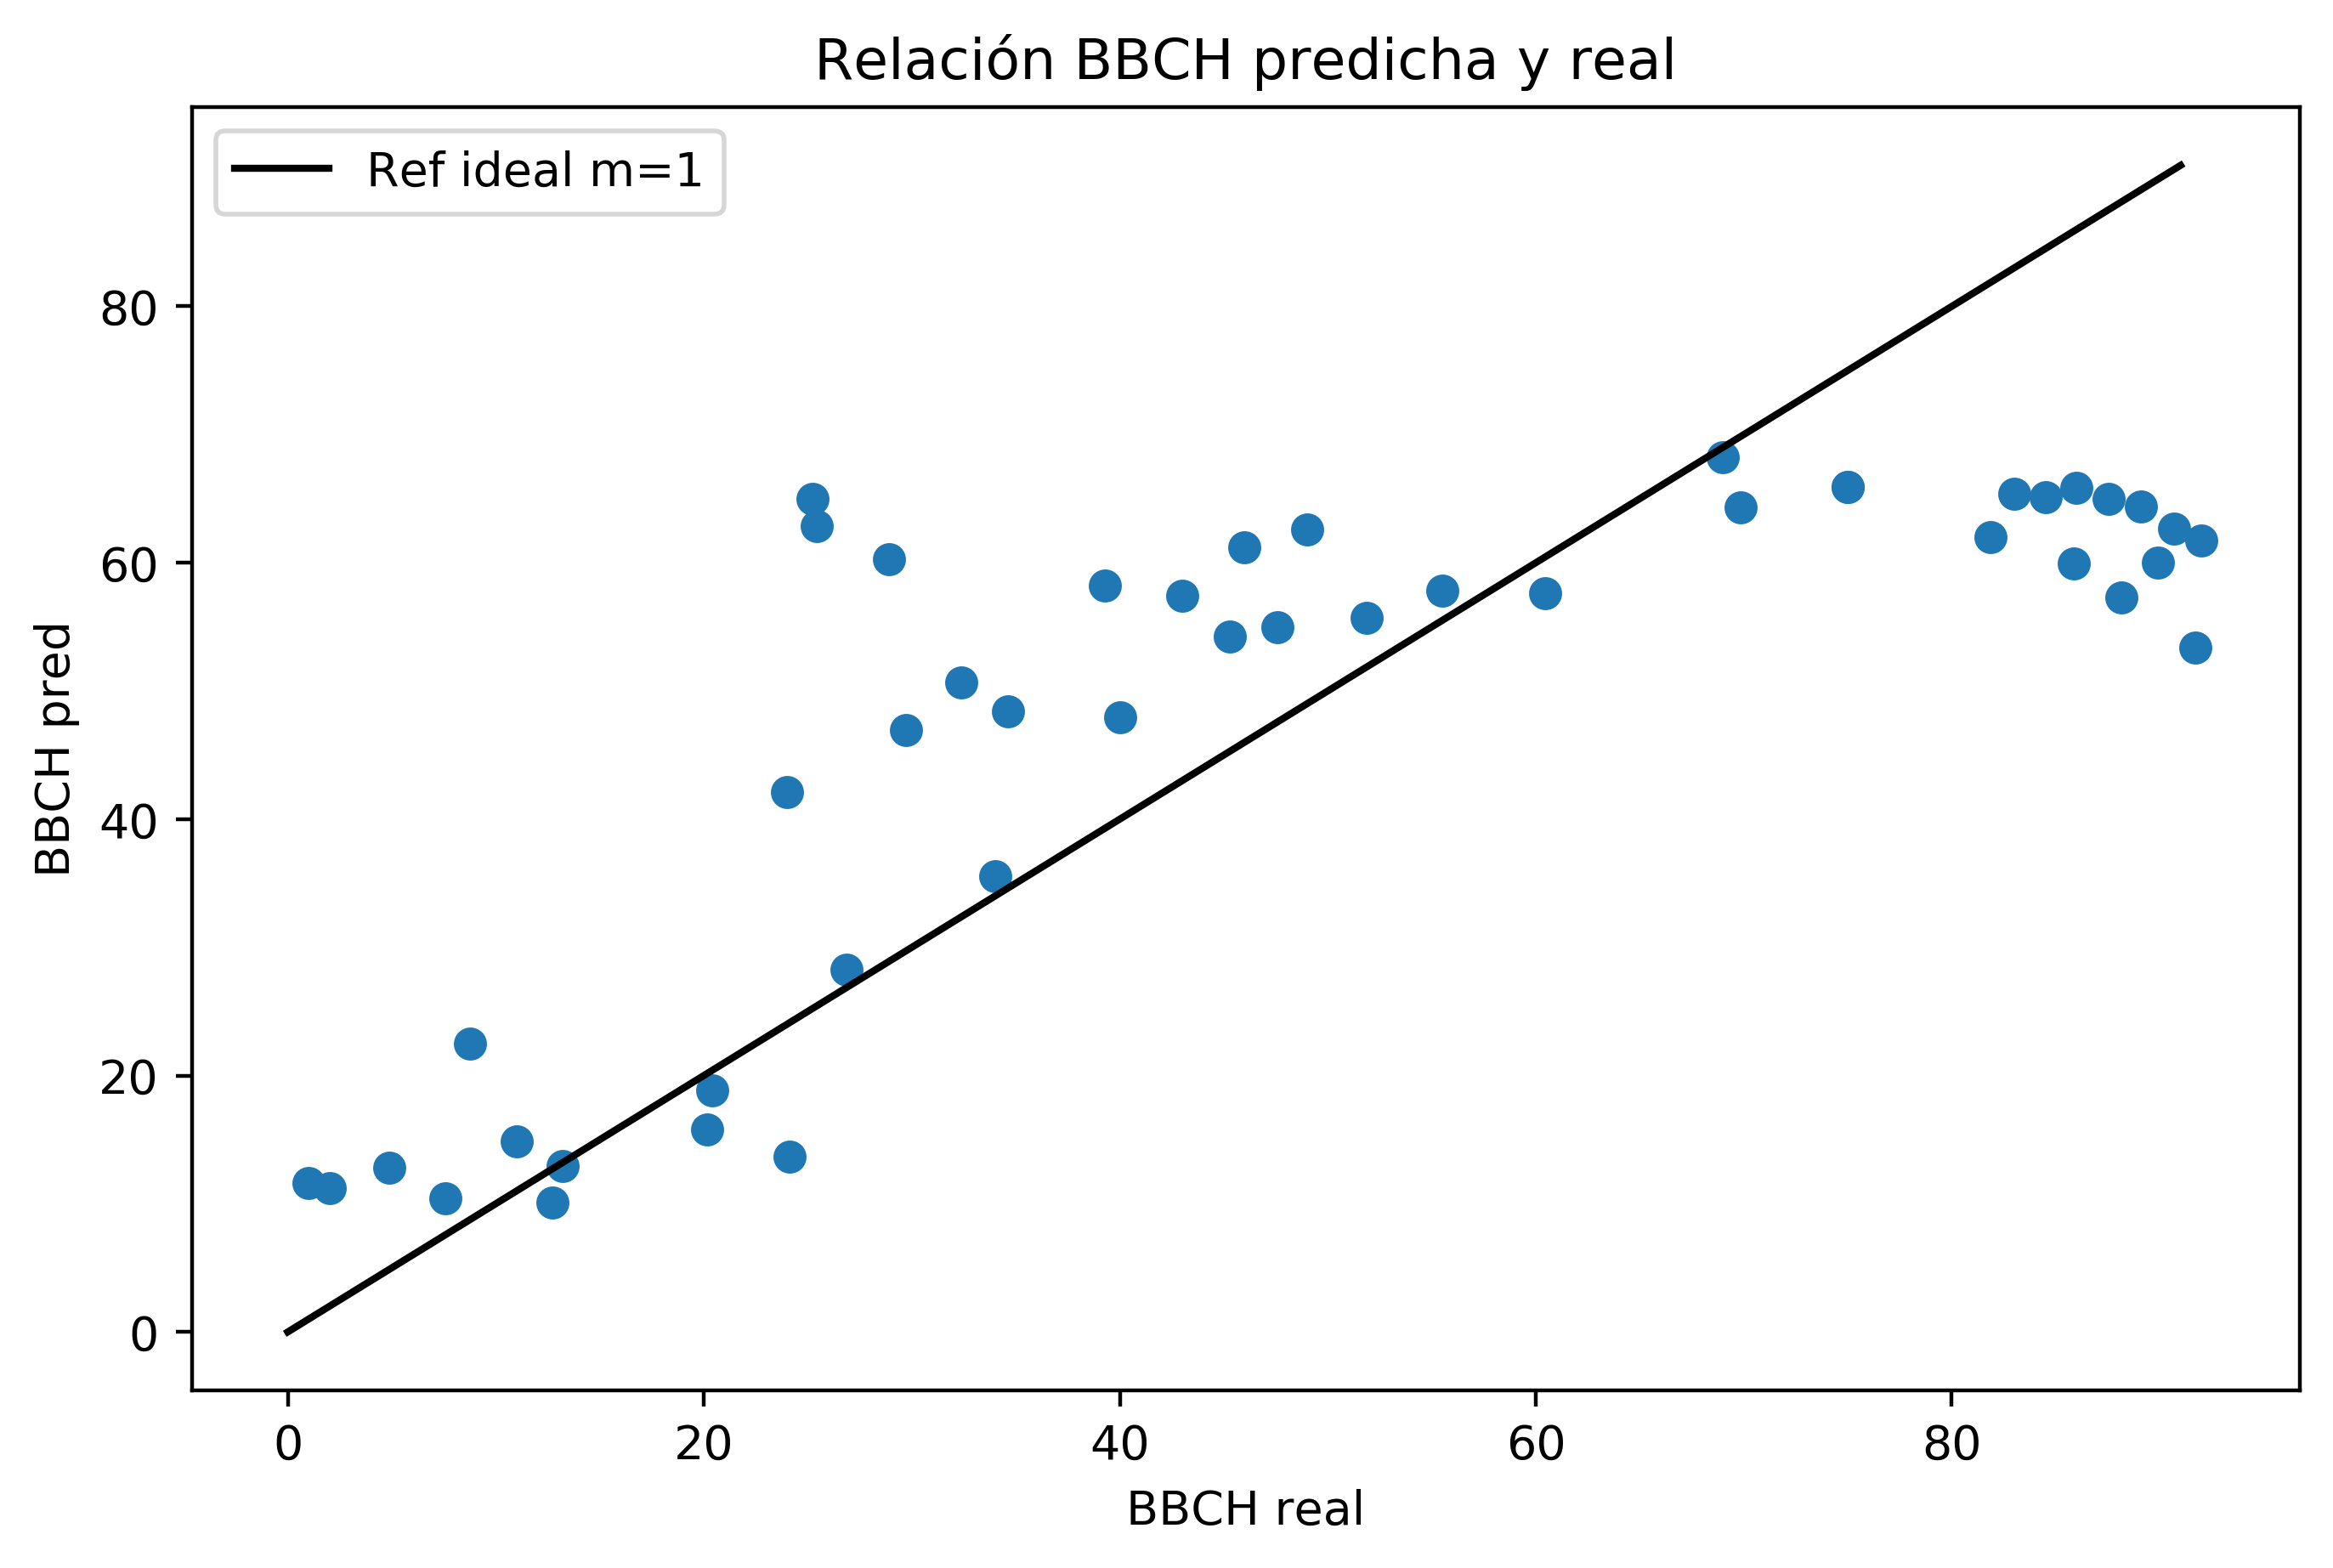
\includegraphics[width=0.95\linewidth]{archivos/tfg/Pixel/BBCH_RELACION_BIEN}
\captionof{figure}{Relación de la salida predicha y la verdad de tierra del modelo para estimación de \gls{bbch}.\label{fig:p_rel_b}}
\end{subfigure}
\begin{subfigure}{.7\textwidth}
\centering
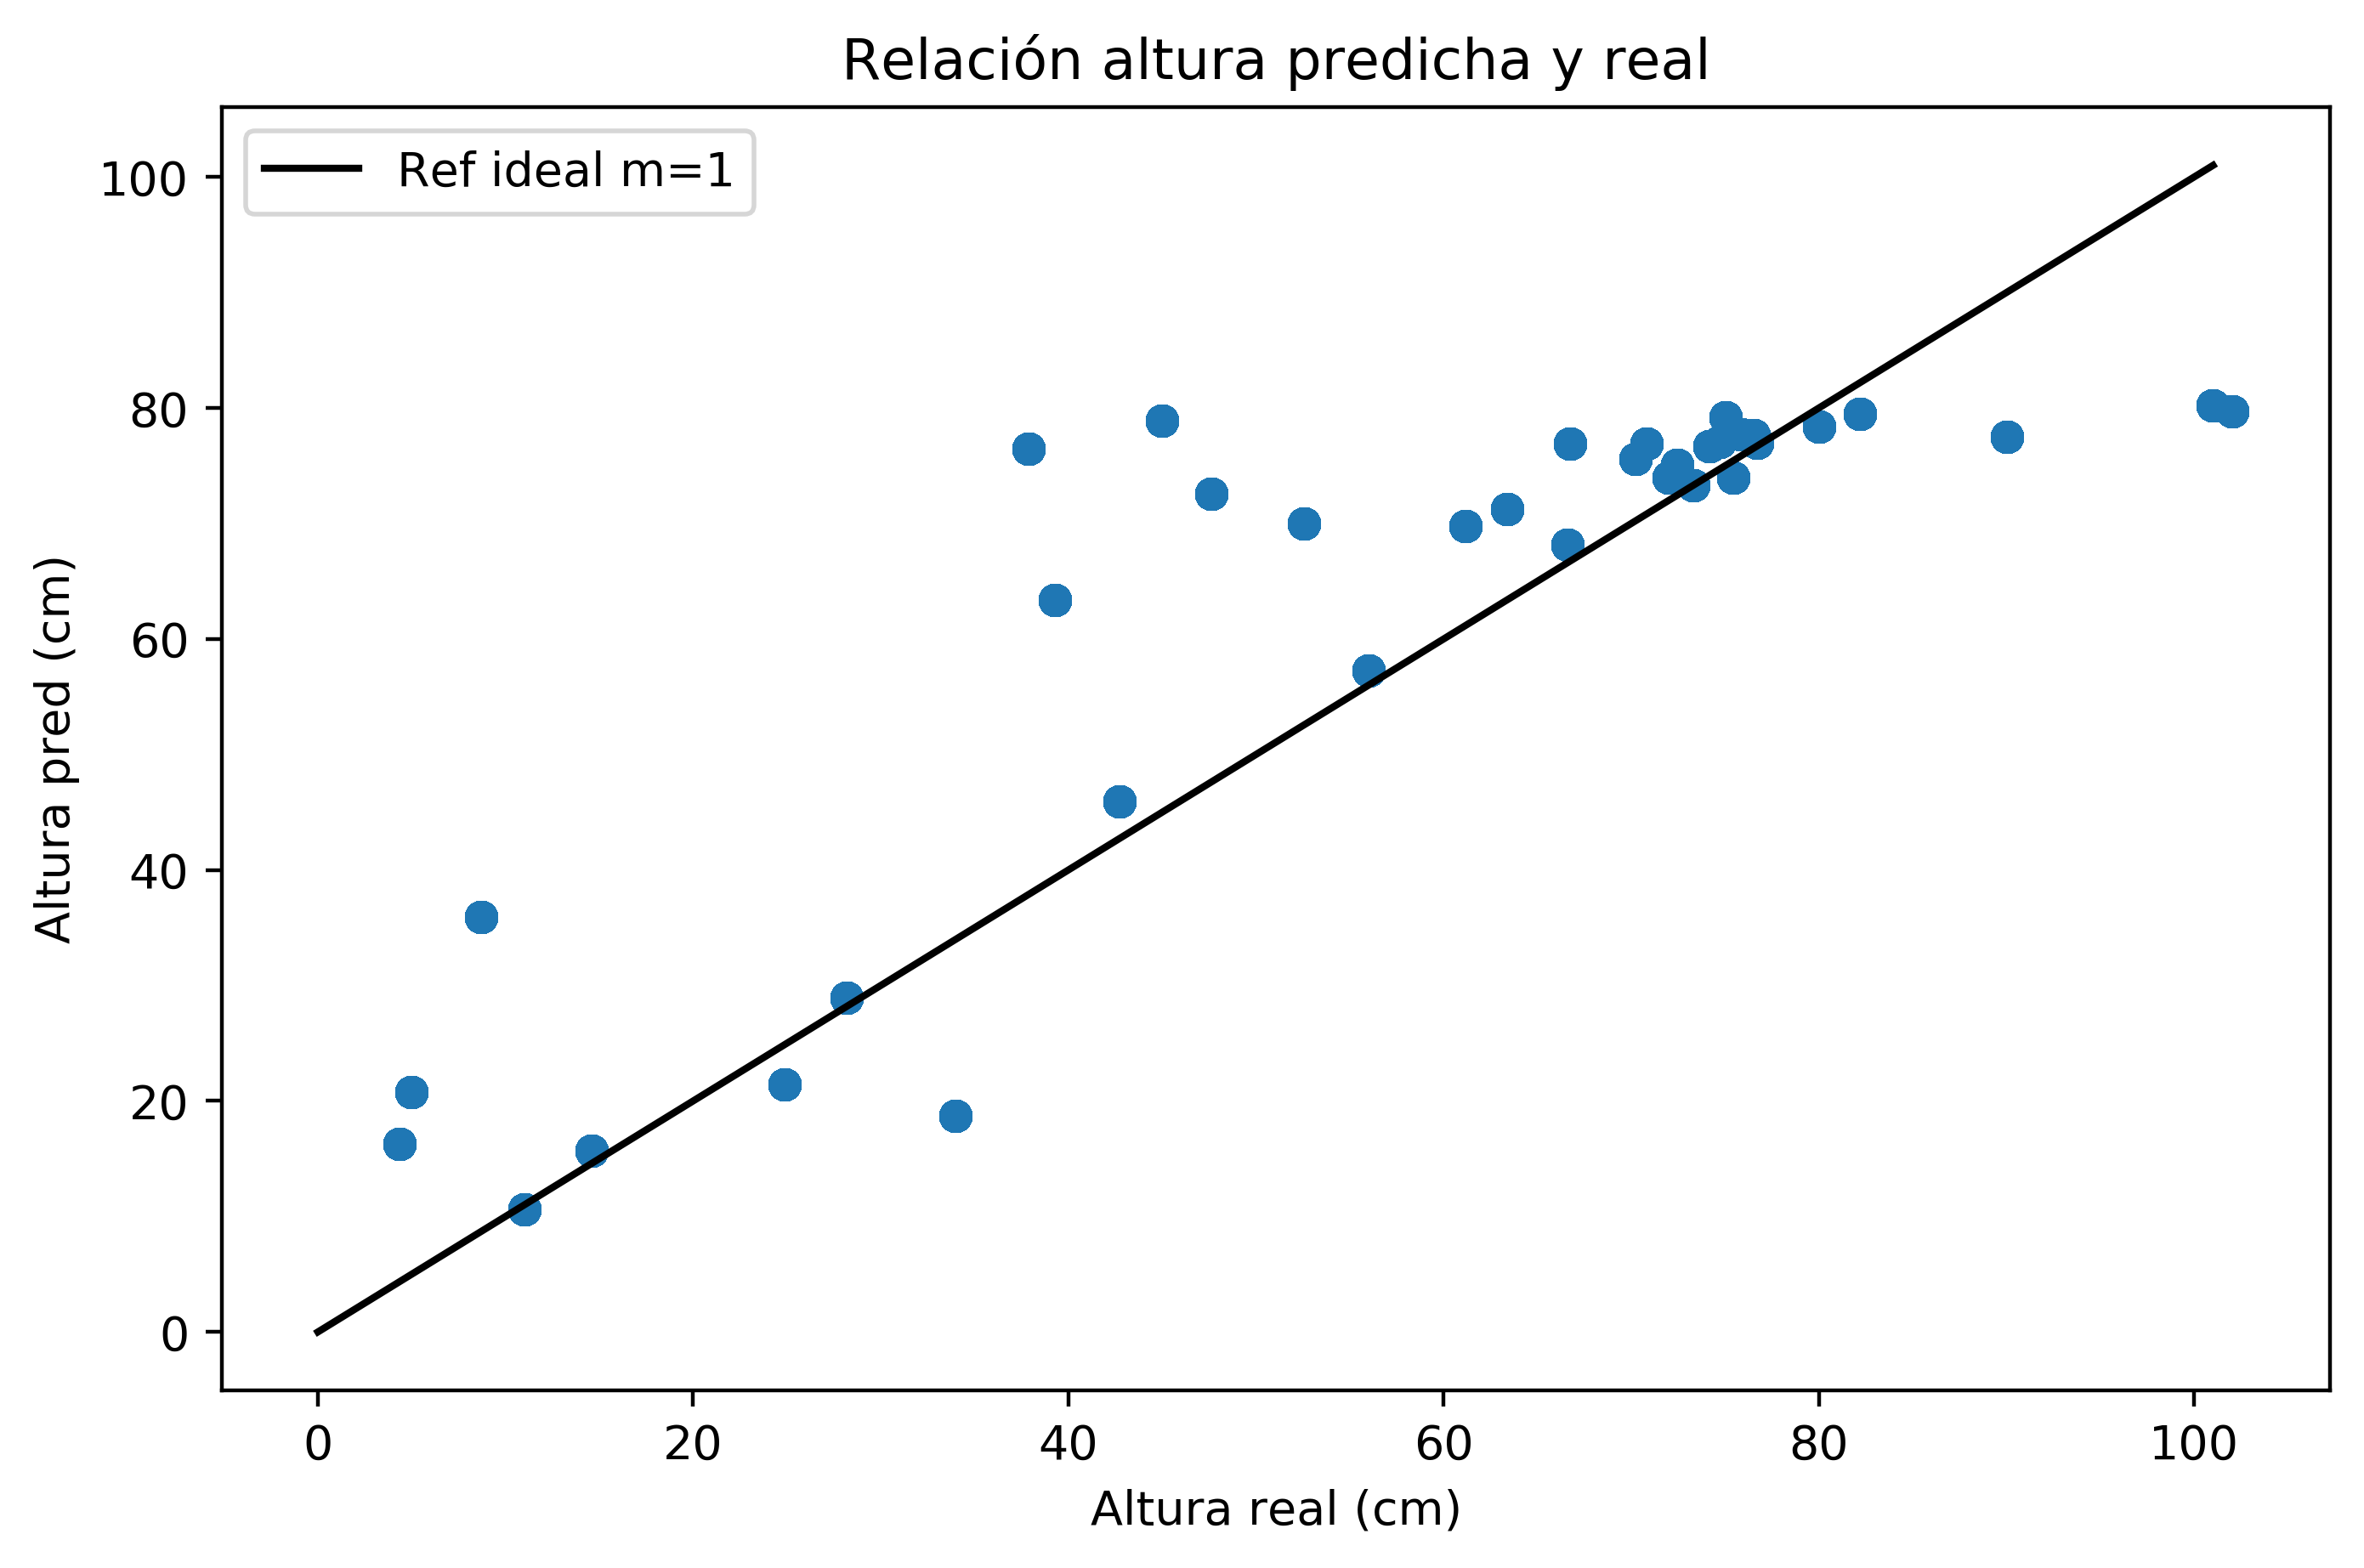
\includegraphics[width=0.95\linewidth]{archivos/tfg/Pixel/H_RELACION_BIEN}
\captionof{figure}{Relación de la salida predicha y la verdad de tierra del modelo para estimación de la altura. \label{fig:p_rel_h}}
\end{subfigure}
\captionof{figure}{Relación de la salida predicha y la verdad de tierra de los modelos de salidas independientes. \label{fig:p_rel_2}}
\end{figure}

% Una figura con dos imágenes
\begin{figure}[H]
\centering
\begin{subfigure}{0.7\textwidth}
  \centering
  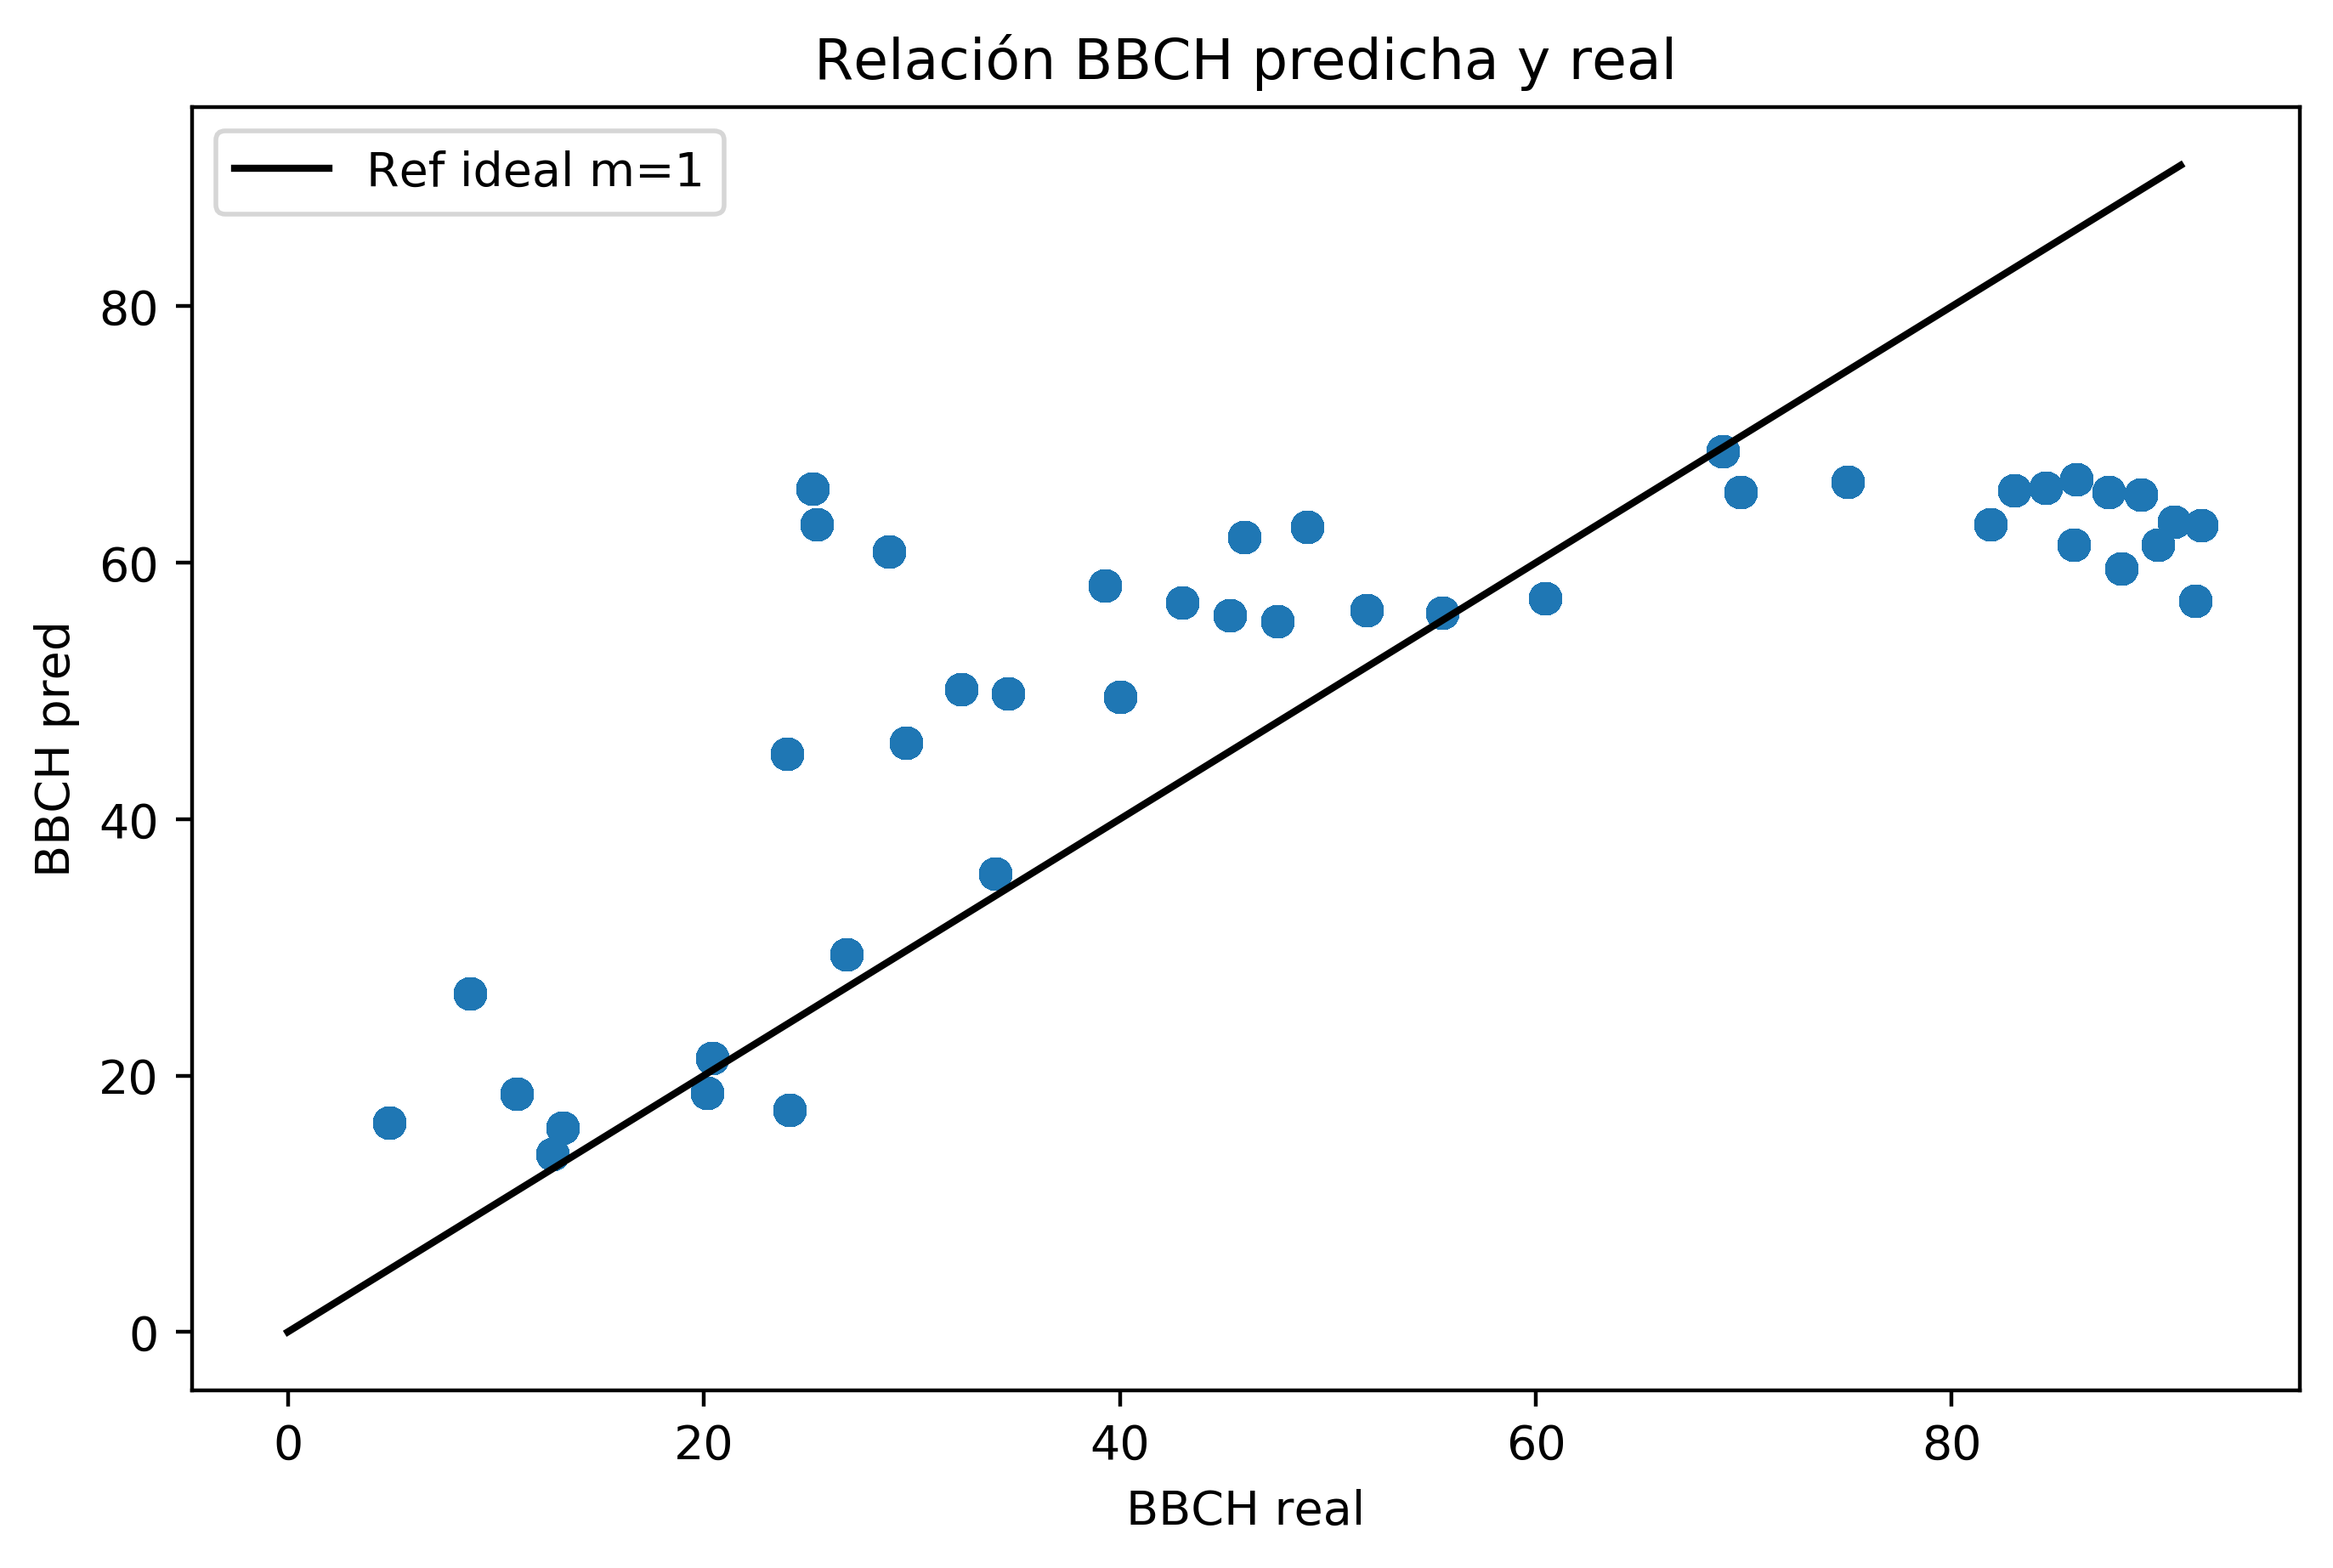
\includegraphics[width=0.95\linewidth]{archivos/tfg/Pixel/BBCHH_RELACION_BIEN_b}
  \caption{Relación de la salida predicha y la verdad de tierra del modelo de doble salida para la estimación de \gls{bbch}. \label{fig:p_rel_bh_b}}
\end{subfigure}
\begin{subfigure}{0.7\textwidth}
  \centering
  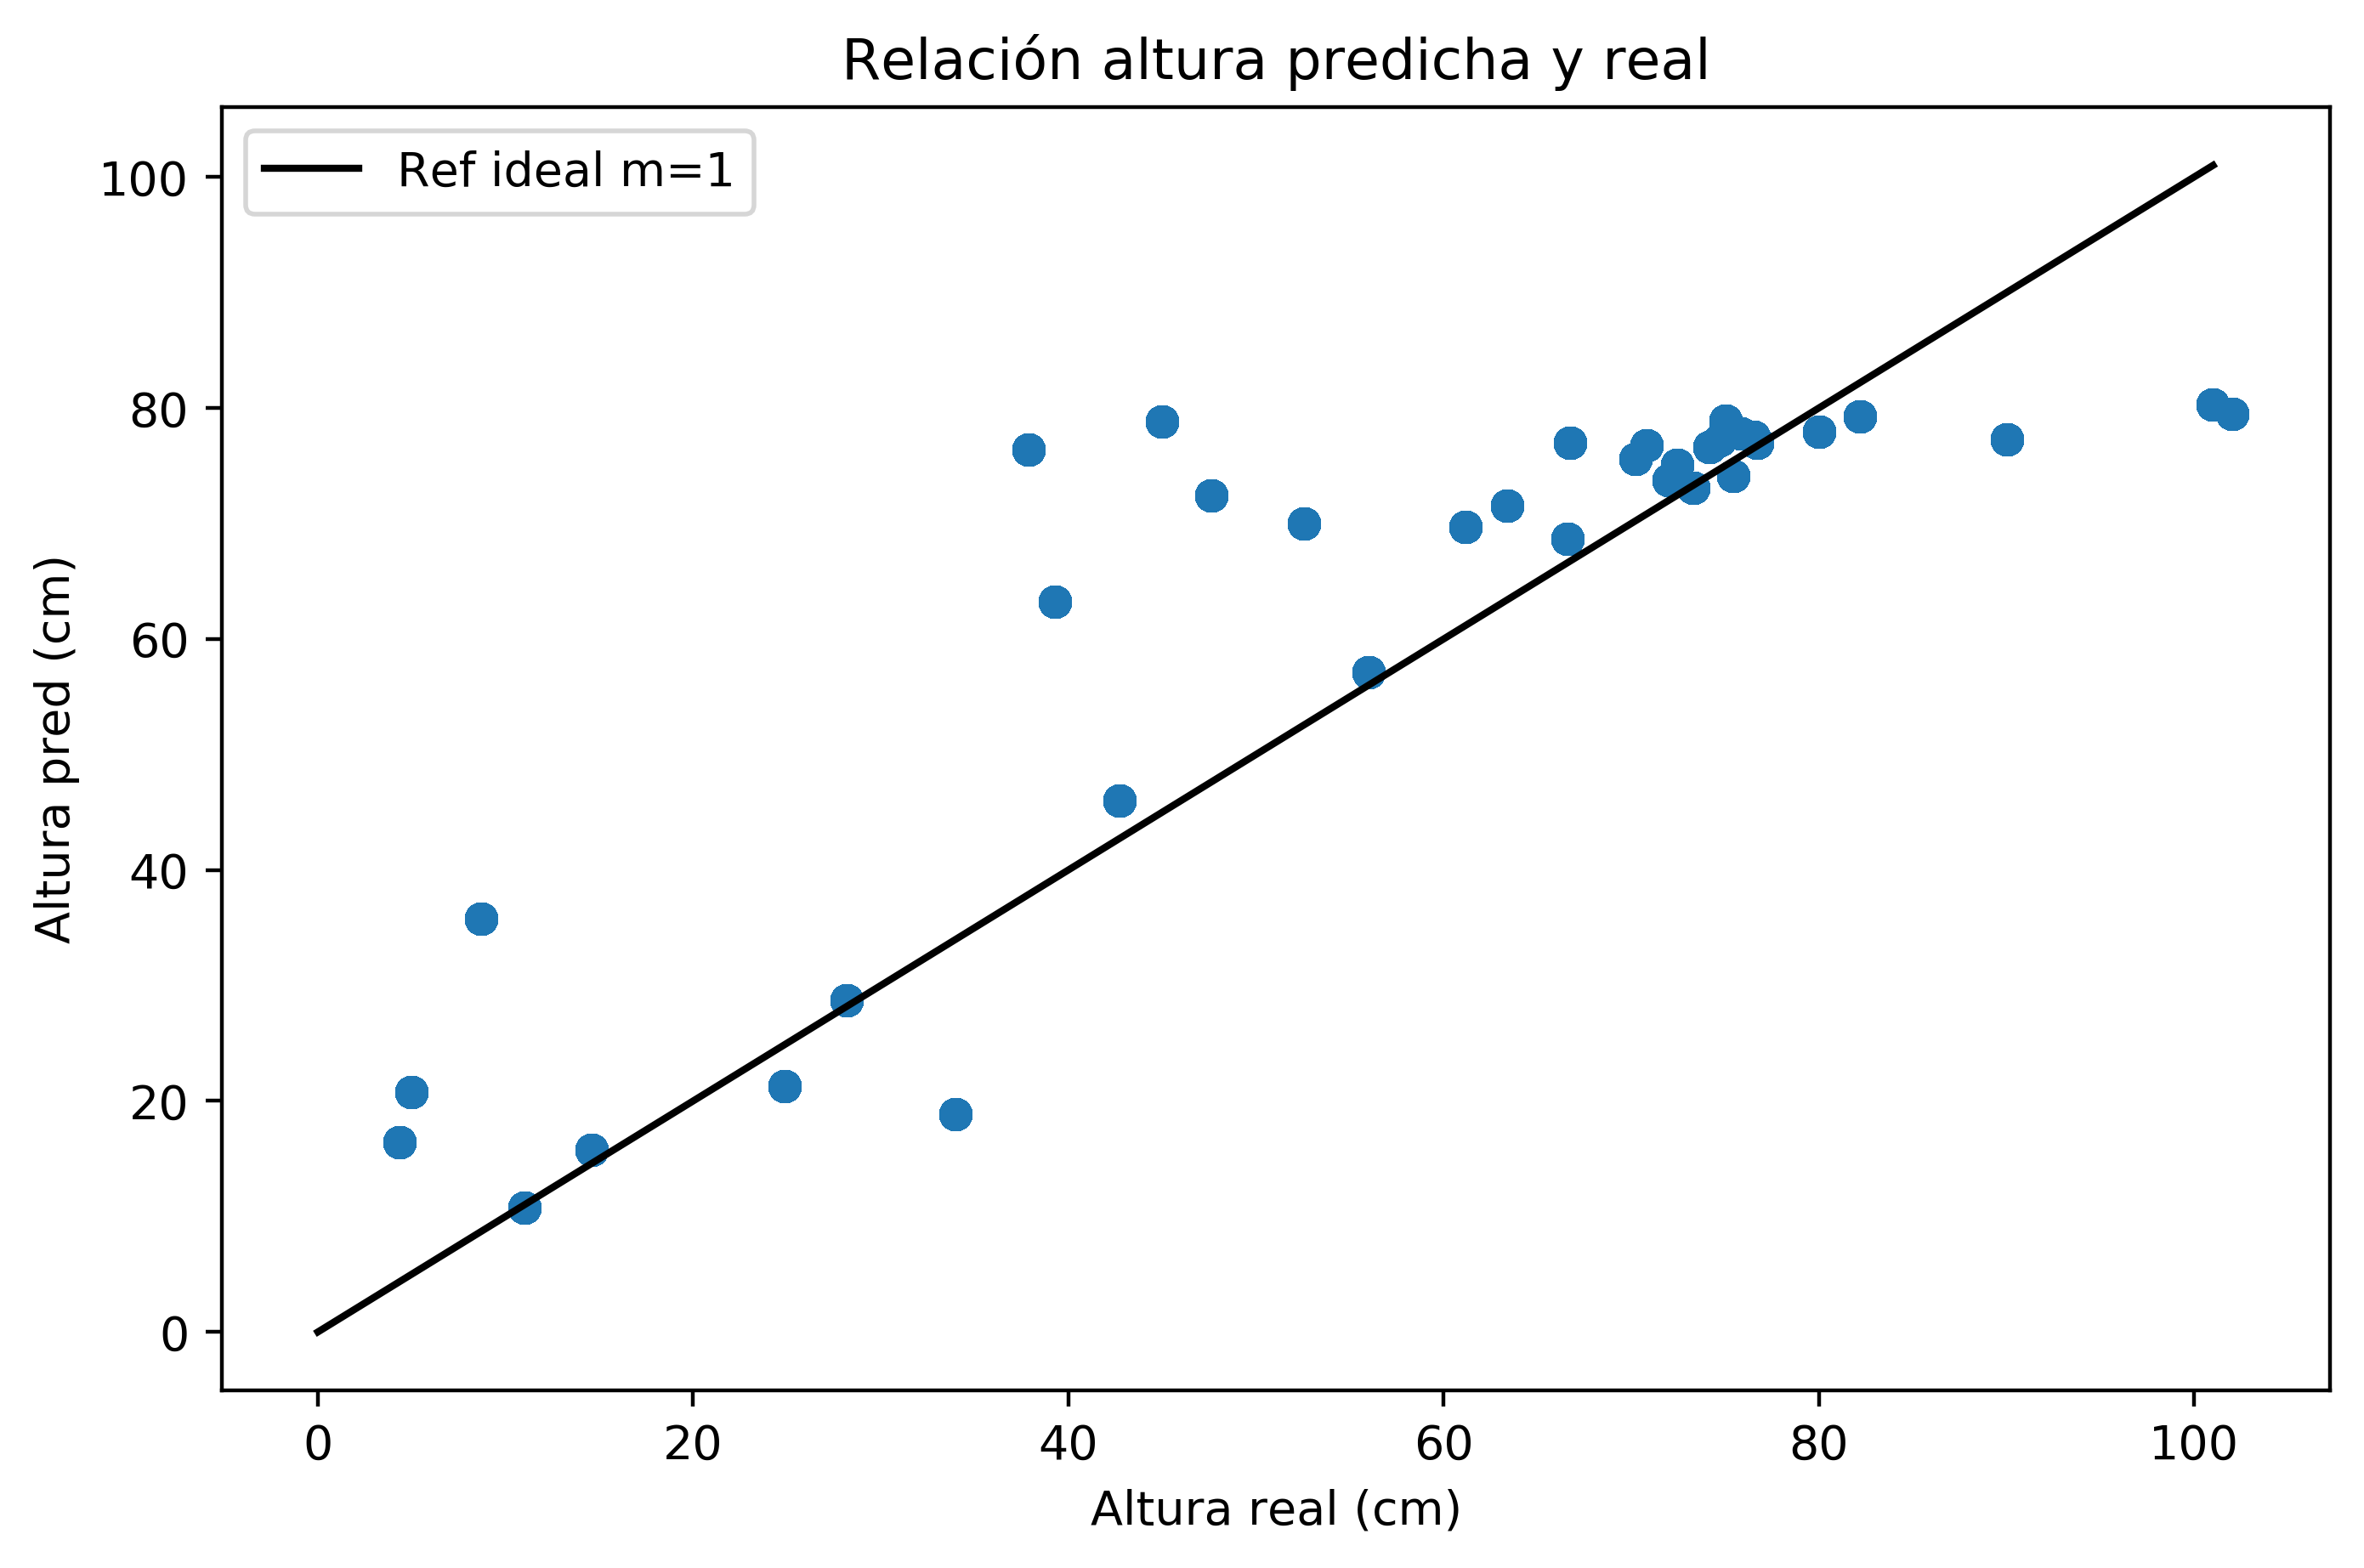
\includegraphics[width=0.95\linewidth]{archivos/tfg/Pixel/BBCHH_RELACION_BIEN_H}
  \caption{Relación de la salida predicha y la verdad de tierra del modelo de doble salida para la estimación de la altura\label{fig:p_rel_bh_h}}
\end{subfigure}
\caption{Relación de la salida predicha y la verdad de tierra del modelo de doble salida para la estimación de \gls{bbch} y la altura. \label{fig:p_rel_bh}}
\end{figure}

\par A parte de la evaluación con descriptores estadísticos que se realizan a la hora de comparar los dos métodos, se realiza una evaluación de los datos de entrada utilizados. La tabla \ref{tab:p_imp_f} representa el peso que tiene cada una de las variables de entrada en el modelo generado para cada uno de los 3 casos tratados. 

\begin{table}[h]
\centering
\begin{tabular}{l|ccc}
               & \gls{bbch} & Altura & \gls{bbch}\&Altura \\ \hline \hline
VV             & 0.19 & 0.16   & 0.19         \\
VH             & 0.61 & 0.61   & 0.59         \\
Ratio VH/VV    & 0.19 & 0.23   & 0.22         
     
\end{tabular}
\caption{Influencia de los parámetros de entrada en el modelo de estimación. \label{tab:p_imp_f}}
\end{table}
%%%%%%%%%%%%%%%%%%%%%%%%%%%%%%%%%%%%%%%%%%%
%%%%%%%%%%%%%%%%%%%%%%%%%%%%%%%%%%%%%%%%%%%
%%%%%%%%%%%%%%%%%%%%%%%%%%%%%%%%%%%%%%%%%%%
\section{Comparativa de métodos}
\par La evaluación general de resultados realizada es la comparación entre los dos métodos de procesamiento de datos de entrada mencionados: a nivel de parcela o de pixel. En las siguientes tablas se pueden ver la evaluación de los resultados, divididos en entradas a nivel de parcela ~\ref{tab:errorpc} y a nivel de pixel ~\ref{tab:errorpx}, según los índices estadísticos de \gls{mae}, \gls{rmse} y el coeficiente de determinación ($R^2$). Ambos conjuntos corresponden al mejor caso de cada método, esto es, habiendo seleccionado sus parámetros de entrada óptimos en cuanto a número de variables y set de parcelas de entrenamiento, y habiendo optimizado también los parámetros del regresor.

\begin{table}[h]
\centering
\begin{tabular}{lccc}
\multicolumn{4}{c}{Datos de entrada a nivel de parcela}                            \\ \hline \hline
\multicolumn{1}{l|}{}                            & \gls{bbch}  & Altura & \gls{bbch}\&Altura \\ \cline{2-4} 
\multicolumn{1}{l|}{$R^2$}                       & 0.74  & 0.65   & 0.70 \\
\multicolumn{1}{l|}{\gls{rmse}} 				 & 15.39 & 17.87  & 15.69 \\
\multicolumn{1}{l|}{\gls{mae}}  				 & 11.13 & 14.21  & 12.63       
\end{tabular}
\caption{Índices estadísticos de las predicciones con datos de entrada a nivel de parcela. \label{tab:errorpc}}
\end{table}

\begin{table}[h]
\centering
\begin{tabular}{lccc}
\multicolumn{4}{c}{Datos de entrada a nivel de pixel}                            \\ \hline \hline
\multicolumn{1}{l|}{}                            & \gls{bbch}  & Altura & \gls{bbch}\&Altura \\ \cline{2-4} 
\multicolumn{1}{l|}{$R^2$}                       & 0.45  & 0.52   & 0.45         \\
\multicolumn{1}{l|}{\gls{rmse}} 				 & 22.23 & 19.89  & 21.17        \\
\multicolumn{1}{l|}{\gls{mae}}  				 & 17.26 & 15.64  & 16.58       
\end{tabular}
\caption{Índices estadísticos de las predicciones con datos de entrada a nivel de pixel.\label{tab:errorpx}}
\end{table}

\par Como se puede observar, para las 3 posibles salidas para las que se han diseñado los modelos, el método que emplea datos de entrada a nivel de parcela consigue notablemente mejores resultados. Se obtienen valores de coeficiente de determinación más cercanos a 1, valor ideal, apreciándose en el modelo de predicción de \gls{bbch} una mejora para el caso de parcelas de un 64.4\% con respecto al de pixel. Lo mismo ocurre en los índices de error, cuyo valor óptimo es 0: se obtienen valores inferiores para el método a nivel de parcela en todos los casos estudiados.
\\
\par Los mejores resultados obtenidos para el procesamiento a nivel de parcelas pueden recaer en que todos los datos recogidos de verdad de tierra se presentan por parcelas, por lo que no existen unos datos para contrastar cada pixel extraído de la información de satélite con el terreno. Dentro de cada parcela el cultivo no tiene porqué desarrollarse de manera homogénea, pero la información recibida de este consta del valor de \gls{bbch} (con el requisito de ser el correcto para al menos el 50\% del cultivo) y la altura generalizados por parcela, además de los máximos y mínimos de cada uno, por lo que las variaciones que se puede hallar en distintas zonas del cultivo no se tienen en cuenta. Por ello, el método de pixel implementado asigna un solo valor de salida para conjuntos de píxeles de la misma parcela, los cuales pueden estar representando unos niveles de \gls{bbch} o altura distintos, y esto conlleva un ajuste del modelo erróneo y, por tanto, peores índices estadísticos de evaluación. Aún así, este método no ha sido descartado, ya que el análisis a nivel de pixel es de gran interés para detectar esas variaciones de desarrollo de un cultivo dentro de una misma parcela. 